% Choose the language of your thesis passing 'french' or 'english' as
% \documentclass option.
% Note1: The 'page de garde' will always be written in French.
% Note2: You will have an error if you change the language of the document and
%        compile it without cleaning the auxiliary files. Compiling it again
%        should solve the problem.
\documentclass[english,a4paper,11pt,twoside]{StyleThese}
\newcommand{\included}{}
\usepackage{pdfpages}

\usepackage{amsmath,amssymb}             % AMS Math
\usepackage[T1]{fontenc}
\usepackage[utf8x]{inputenc}
\usepackage{babel}
\usepackage{datetime}

\usepackage{array}
% \newcolumntype{x}[1]{>{\centering\arraybackslash\hspace{0pt}}p{#1}}
\newcolumntype{x}[1]{>{\centering\let\newline\\\arraybackslash\hspace{0pt}}p{#1}}

\usepackage{lmodern}
\usepackage{tabularx}
%\usepackage{tabular}
\usepackage{multirow}
\usepackage{enumitem}
\usepackage{subcaption}
\usepackage{siunitx}
% \usepackage{algorithm}
\usepackage{algpseudocode}
\usepackage{hhline}
\usepackage[left=1.2in,right=1.0in,top=1.1in,bottom=1.1in,includefoot,includehead,headheight=13.6pt]{geometry}
\renewcommand{\baselinestretch}{1.05}
% Table of contents for each chapter

\usepackage[nottoc, notlof, notlot]{tocbibind}
\usepackage{minitoc}
\setcounter{minitocdepth}{2}
\mtcindent=15pt
% Use \minitoc where to put a table of contents

\usepackage{aecompl}

% Glossary / list of abbreviations

\usepackage[intoc]{nomencl}
\iftoggle{ThesisInEnglish}{%
\renewcommand{\nomname}{Glossary}
}{ %
\renewcommand{\nomname}{Liste des Abréviations}
}

\makenomenclature

% My pdf code

\usepackage{ifpdf}

\ifpdf
  \usepackage{graphicx}
  \usepackage[a4paper,pagebackref,hyperindex=true]{hyperref}
  \usepackage{tikz}
  \usetikzlibrary{arrows,shapes,calc}
\else
  \usepackage{graphicx}
  \DeclareGraphicsExtensions{.ps,.eps}
  \usepackage[a4paper,dvipdfm,pagebackref,hyperindex=true]{hyperref}
\fi

\graphicspath{{.}{images/}}

%% nicer backref links. NOTE: The flag ThesisInEnglish is used to define the
% language in the back references. Read more about it in These.tex

\iftoggle{ThesisInEnglish}{%
\renewcommand*{\backref}[1]{}
\renewcommand*{\backrefalt}[4]{%
\ifcase #1 %
(Not cited.)%
\or
(Cited in page~#2.)%
\else
(Cited in pages~#2.)%
\fi}
\renewcommand*{\backrefsep}{, }
\renewcommand*{\backreftwosep}{ and~}
\renewcommand*{\backreflastsep}{ and~}
}{%
\renewcommand*{\backref}[1]{}
\renewcommand*{\backrefalt}[4]{%
\ifcase #1 %
(Non cité.)%
\or
(Cité en page~#2.)%
\else
(Cité en pages~#2.)%
\fi}
\renewcommand*{\backrefsep}{, }
\renewcommand*{\backreftwosep}{ et~}
\renewcommand*{\backreflastsep}{ et~}
}

% Links in pdf
\usepackage{color}
\definecolor{linkcol}{rgb}{0,0,0.4} 
\definecolor{citecol}{rgb}{0.5,0,0} 
\definecolor{linkcol}{rgb}{0,0,0} 
\definecolor{citecol}{rgb}{0,0,0}
% Change this to change the informations included in the pdf file

\hypersetup
{
bookmarksopen=true,
pdftitle=Human-Aware Robot Task Planning: Theory of Mind and Anticipation of Human Decisions and Actions,
pdfauthor=Anthony Favier, %auteur du document
pdfsubject=Thesis, %sujet du document
%pdftoolbar=false, %barre d'outils non visible
pdfmenubar=true, %barre de menu visible
pdfhighlight=/O, %effet d'un clic sur un lien hypertexte
colorlinks=true, %couleurs sur les liens hypertextes
pdfpagemode=None, %aucun mode de page
pdfpagelayout=SinglePage, %ouverture en simple page
pdffitwindow=true, %pages ouvertes entierement dans toute la fenetre
linkcolor=linkcol, %couleur des liens hypertextes internes
citecolor=citecol, %couleur des liens pour les citations
urlcolor=linkcol %couleur des liens pour les url
}

% definitions.
% -------------------

\setcounter{secnumdepth}{3}
\setcounter{tocdepth}{2}

% Some useful commands and shortcut for maths:  partial derivative and stuff

\newcommand{\pd}[2]{\frac{\partial #1}{\partial #2}}
\def\abs{\operatorname{abs}}
\def\argmax{\operatornamewithlimits{arg\,max}}
\def\argmin{\operatornamewithlimits{arg\,min}}
\def\diag{\operatorname{Diag}}
\newcommand{\eqRef}[1]{(\ref{#1})}

\usepackage[figuresleft]{rotating}                    % Sideways of figures & tables
%\usepackage{bibunits}
%\usepackage[sectionbib]{chapterbib}          % Cross-reference package (Natural BiB)
%\usepackage{natbib}                  % Put References at the end of each chapter
                                         % Do not put 'sectionbib' option here.
                                         % Sectionbib option in 'natbib' will do.


% \usepackage{txfonts}                     % Public Times New Roman text & math font
% \usepackage[ED=MITT-InfoTel, Ets=UT3]{tlsflyleaf}
\usepackage{fancyhdr}                    % Fancy Header and Footer  
%%% Fancy Header %%%%%%%%%%%%%%%%%%%%%%%%%%%%%%%%%%%%%%%%%%%%%%%%%%%%%%%%%%%%%%%%%%
% Fancy Header Style Options

\pagestyle{fancy}                       % Sets fancy header and footer
\fancyfoot{}                            % Delete current footer settings

%\renewcommand{\chaptermark}[1]{         % Lower Case Chapter marker style
%  \markboth{\chaptername\ \thechapter.\ #1}}{}} %

%\renewcommand{\sectionmark}[1]{         % Lower case Section marker style
%  \markright{\thesection.\ #1}}         %

\fancyhf{}
\fancyhead[LE,RO]{\bfseries\thepage}    % Page number (boldface) in left on even
% pages and right on odd pages
% \renewcommand{\chaptermark}[1]{\markboth{\nouppercase{\thechapter.\ #1}}{}}
\fancyhead[RE]{\bfseries\nouppercase{\leftmark}}      % Chapter in the right on even pages
\fancyhead[LO]{\bfseries\nouppercase{\rightmark}}     % Section in the left on odd pages

\let\headruleORIG\headrule
\renewcommand{\headrule}{\color{black} \headruleORIG}
\renewcommand{\headrulewidth}{1.0pt}
\usepackage{colortbl}
\arrayrulecolor{black}

\fancypagestyle{plain}{
  \fancyhead{}
  \fancyfoot{}
  \renewcommand{\headrulewidth}{0pt}
}

%\usepackage{MyAlgorithm}
%\usepackage[noend]{MyAlgorithmic}

%%% Clear Header %%%%%%%%%%%%%%%%%%%%%%%%%%%%%%%%%%%%%%%%%%%%%%%%%%%%%%%%%%%%%%%%%%
% Clear Header Style on the Last Empty Odd pages
\makeatletter

\def\cleardoublepage{\clearpage\if@twoside \ifodd\c@page\else%
  \hbox{}%
  \thispagestyle{empty}%              % Empty header styles
  \newpage%
  \if@twocolumn\hbox{}\newpage\fi\fi\fi}

\makeatother
 
%%%%%%%%%%%%%%%%%%%%%%%%%%%%%%%%%%%%%%%%%%%%%%%%%%%%%%%%%%%%%%%%%%%%%%%%%%%%%%% 
% Prints your review date and 'Draft Version' (From Josullvn, CS, CMU)
\newcommand{\reviewtimetoday}[2]{\special{!userdict begin
    /bop-hook{gsave 20 710 translate 45 rotate 0.8 setgray
      /Times-Roman findfont 12 scalefont setfont 0 0   moveto (#1) show
      0 -12 moveto (#2) show grestore}def end}}
% You can turn on or off this option.
% \reviewtimetoday{\today}{Draft Version}
%%%%%%%%%%%%%%%%%%%%%%%%%%%%%%%%%%%%%%%%%%%%%%%%%%%%%%%%%%%%%%%%%%%%%%%%%%%%%%% 

\newenvironment{maxime}[1]
{
\vspace*{0cm}
\hfill
\begin{minipage}{0.5\textwidth}%
%\rule[0.5ex]{\textwidth}{0.1mm}\\%
\hrulefill $\:$ {\bf #1}\\
%\vspace*{-0.25cm}
\it 
}%
{%

\hrulefill
\vspace*{0.5cm}%
\end{minipage}
}

\let\minitocORIG\minitoc
\renewcommand{\minitoc}{\minitocORIG \vspace{1.5em}}

\usepackage{multirow}
%\usepackage{slashbox}

\newenvironment{bulletList}%
{ \begin{list}%
	{$\bullet$}%
	{\setlength{\labelwidth}{25pt}%
	 \setlength{\leftmargin}{30pt}%
	 \setlength{\itemsep}{\parsep}}}%
{ \end{list} }

\newtheorem{definition}{Definition}
\renewcommand{\epsilon}{\varepsilon}

% centered page environment

\newenvironment{vcenterpage}
{\newpage\vspace*{\fill}\thispagestyle{empty}\renewcommand{\headrulewidth}{0pt}}
{\vspace*{\fill}}

\usepackage{tablefootnote}

\newcommand{\mysection}[1]{%
    \section*{#1}%
    \addcontentsline{toc}{section}{#1}%
    \markright{#1}%
}
\usepackage[disable,colorinlistoftodos,prependcaption,textsize=tiny]{todonotes}
\usepackage{xargs}   % Use more than one optional parameter in a new commands
\usepackage{xcolor}  % Coloured text
\usepackage{xspace}

\usepackage{hyperref}
\usepackage{amsmath}
\usepackage{amssymb}
\usepackage{bbm}
%\usepackage{mathbbol}

\usepackage{longtable}

\usepackage{booktabs}
\usepackage{courier}

\usepackage{moreverb}

% \usepackage[bottom]{footmisc}
\definecolor{lightgray}{gray}{0.5}

\usepackage{listings}
\usepackage[normalem]{ulem}
\useunder{\uline}{\ul}{}

\newtheorem{theorem}{Theorem}

\usepackage{algorithm}
% \usepackage[noend]{algpseudocode} 
% limit indentation in algorithms
% \algrenewcommand\algorithmicindent{1.0em}%
% \algnewcommand{\IIf}[1]{\State\algorithmicif\ #1\ \algorithmicthen}
% \algnewcommand{\EndIIf}{\unskip\ \algorithmicend\ \algorithmicif}

\newcommand*{\field}[1]{\mathbb{#1}}%

%%%%%%%%%%%%%%%%%%%%%%%%
%	 listing formats   %
%%%%%%%%%%%%%%%%%%%%%%%%

\lstdefinestyle{HatpPlan}{
  language=C,
  commentstyle=\itshape\color{green!25!black},
}

\lstdefinestyle{OwlTurtle}{
  language=C,
  keywordstyle=\bfseries\color{darkgray},
  morekeywords={rdf:type, rdfs:domain, rdfs:subPropertyOf, rdfs:range, :hasSubtask, :DecompositionUsedBy, rdfs:subClassOf, :hasDecomposition, owl:inverseOf},
  alsoletter=:
}

\lstdefinestyle{OwlTurtle_indiv}{
  language=C,
  keywordstyle=\bfseries\color{darkgray},
  morekeywords={rdf, rdfs, type, domain, subPropertyOf, range, hasSubtask, DecompositionUsedBy, subClassOf, hasDecomposition, Cut_hasParameter, A, V, K, hasColor, hasCadModel, isOn, isInRegion, isAtEndOfPath, isAtLeftOfPath, hasAtRight, isInFrontOf, objectActedOn, eventOccursAt, startTime}
}

\lstdefinestyle{Labels}{
  language=C,
  basicstyle = \fontencoding{T1}\ttfamily \color{black} \footnotesize
}

%%%%%%%%%%%%%%%%%%%%%%%%%%%%%%%%%%%%%%%%%%%%%%%%%%%%%%%%%%
%                         NEW                            %
%%%%%%%%%%%%%%%%%%%%%%%%%%%%%%%%%%%%%%%%%%%%%%%%%%%%%%%%%%

\newcommandx{\chapabstract}[1]{\textbf{\textit{#1}}}


\newcommandx{\agent}{\varphi}
\newcommandx{\agentstate}[2][1,2,usedefault=]{\sigma^{#1}_{#2}}
\newcommandx{\agentmodel}[1][1,usedefault=]{\mathcal{M}^{#1}}
\newcommandx{\agenda}[2][1,2,usedefault=]{d^{#1}_{#2}}
\newcommandx{\partialplan}[2][1,2,usedefault=]{\pi^{#1}_{#2}}
\newcommandx{\valf}[2][1,2,usedefault=]{val^{#1}_{#2}}
\newcommandx{\obsf}[1][1,usedefault=]{obs_{#1}}
\newcommandx{\locf}[1][1,usedefault=]{loc_{#1}}
\newcommandx{\observable}{\texttt{OBS}}
\newcommandx{\inferable}{\texttt{INF}}




%%%%%%%%%%%%%%%%%%%%%%%%%%%%%%%%%%%%%%%%%%%%%%%%%%%%%%%%%%
%                         OLD                            %
%%%%%%%%%%%%%%%%%%%%%%%%%%%%%%%%%%%%%%%%%%%%%%%%%%%%%%%%%%

%%%%%%%%%%%%%%%%%%%%%%%%
%	  TODO commands    %
%%%%%%%%%%%%%%%%%%%%%%%%

\setlength{\marginparwidth}{3cm}
\newcommandx{\unsure}[2][1=]{\todo[linecolor=red,backgroundcolor=red!25,bordercolor=red,#1]{#2}}
\newcommandx{\change}[2][1=]{\todo[linecolor=blue,backgroundcolor=blue!25,bordercolor=blue,#1]{#2}}
\newcommandx{\info}[2][1=]{\todo[linecolor=olive,backgroundcolor=olive!25,bordercolor=olive,#1]{#2}}
\newcommandx{\improvement}[2][1=]{\todo[linecolor=violet,backgroundcolor=violet!25,bordercolor=violet,#1]{#2}}
\newcommandx{\thiswillnotshow}[2][1=]{\todo[disable,#1]{#2}}

%%%%%%%%%%%%%%%%%%%%%%%%
%	Knowledge bases    %
%%%%%%%%%%%%%%%%%%%%%%%%

\newcommand \kb{K}

% Ontology definition

\newcommand \kbs{\kb_S}
\newcommand \Abox{\mathbb{A}}
\newcommand \Tbox{\mathbb{T}}
\newcommand \Rbox{\mathbb{R}}

\newcommand \propset{P}
\newcommand \classset{T}
\newcommand \indivset{A}
\newcommand \relationset{R}
\newcommand \annotationset{E}

\newcommand \domainset{Dom}
\newcommand \rangeset{Ran}
\newcommand \inclset{Incl}
\newcommand \invset{Inv}
\newcommand \inheritset{C}

\newcommand \indiv{a}
\newcommand \class{t}

\newcommand \labelfunc {\mathcal{L}}
\newcommand \alabel{\mathcal{L}_a}
\newcommand \tlabel{\mathcal{L}_t}
\newcommand \plabel{\mathcal{L}_p}
\newcommand \alabelag[1]{\mathcal{L}_{a#1}}
\newcommand \tlabelag[1]{\mathcal{L}_{t#1}}
\newcommand \plabelag[1]{\mathcal{L}_{p#1}}

\newcommand \subject{s}
\newcommand \property{p}
\newcommand \object{o}
\newcommand \relation{r}

\newcommand{\sparql}{\textsc{sparql}}

% Timeline definition

\newcommand \kbe{\kb_E}
\newcommand \tinterval{\mathcal{T}}
\newcommand \tstart{\tau_s}
\newcommand \tend{\tau_e}
\newcommand \taction{\alpha}

%%%%%%%%%%%%%%%%%%%%%%%%
%	      REG          %
%%%%%%%%%%%%%%%%%%%%%%%%

\newcommand \goalindiv{\indiv_t}
\newcommand \usablepropset{U}
\newcommand \problem{\mathcal{P}}
\newcommand \solution{\mathcal{S}}

\newcommand \costfunc{\mathcal{C}}
\newcommand \varset{X}
\newcommand \var{x}

\newcommand \cost{\mathbbm{c}}
\newcommand \node{\mathbbm{n}}
\newcommand \state{\mathbbm{s}}
\newcommand \action{\mathbbm{a}}

\newcommand \softdiff{\,\delta\,}
\newcommand \harddiff{\,\Delta\,}

\newcommand \symboltable{\mathcal{S}}
\newcommand \matchtable{\mathcal{M}}

\newcommand \us{$\mu$s\xspace}

\newcommand{\tovariable}{\textsc{ToVariable}}
\newcommand{\toquery}{\textsc{ToQuery}}
\newcommand{\sparqlresult}{\textsc{SparqlResult}}
\newcommand{\createchild}{\textsc{CreateChild}}
\newcommand{\actions}{\textsc{Actions}}
\newcommand{\goaltest}{\textsc{GoalTest}}
\newcommand{\typingactions}{\textsc{TypingActions}}
\newcommand{\differenceactions}{\textsc{DifferentiationActions}}

\newcommand{\additions}{\textsc{CreateAddition}}
\newcommand{\typingadditions}{\textsc{TypingAdditions}}
\newcommand{\differenceadditions}{\textsc{DifferentiationAdditions}}
\newcommand{\actingadditions}{\textsc{ActingAdditions}}
\newcommand{\completionadditions}{\textsc{CompletionAdditions}}
\newcommand{\compoundadditions}{\textsc{CompoundAdditions}}
\newcommand{\createtree}{\textsc{CreateTree}}
\newcommand{\getsubtrees}{\textsc{getSubTrees}}

%%%%%%%%%%%%%%%%%%%%%%%%
%	      HTN          %
%%%%%%%%%%%%%%%%%%%%%%%%

\newcommand \tasknetwork{N}
\newcommand \task{n}
\newcommand \primtaskset{Pt}
\newcommand \abstaskset{At}
\newcommand \decomposet{D}
\newcommand \decompo{d}
\newcommand \abstracttask{\upsilon}
\newcommand \HTN{Pl}
\usepackage[acronym]{glossaries}

\makenoidxglossaries

\newacronym{ai}{AI}{Artificial Intelligence}
\newacronym{hhi}{HHI}{Human-Human Interaction}
\newacronym{hci}{HCI}{Human-Computer Interaction}
\newacronym{hri}{HRI}{Human-Robot Interaction}
\newacronym{hrc}{HRC}{Human-Robot Collaboration}
\newacronym{han}{HAN}{Human-Aware Navigation}
\newacronym{cohan}{CoHAN}{Cooperative Human-Aware Navigation}
\newacronym{orca}{ORCA}{Optimal Reciprocal Collision Avoidance}
\newacronym{sfm}{SFM}{Social Force Model}
\newacronym{pomdp}{POMDP}{Partially Observable Markov Decision Process}
\newacronym{mdp}{MDP}{Markov Decision Process}
\newacronym{amm}{AMM}{Agent Markov Model}
\newacronym{ros}{ROS}{Robot Operating System}
\newacronym{hatpehda}{HATP/EHDA}{Human-Aware Task Planner Emulating Human Decisions and Actions}
\newacronym{hatp}{HATP}{Hierarchical Agent-based Task Planner}
\newacronym{tom}{ToM}{Theory of Mind}
\newacronym{htn}{HTN}{Hierarchical Task Network}
\newacronym{inhus}{InHuS}{Intelligent Human Simuator}
\newacronym{imhus}{IMHuS}{Intelligent Multi Human Simuator}
\newacronym{sa}{SA}{Situation Assessment}
\newacronym{del}{DEL}{Dynamic Epistemic Logic}
\newacronym{id}{ID}{Identification}
\newacronym{dag}{DAG}{Directed Acyclic Graph}


\setlength{\belowcaptionskip}{-6pt}

%%%%%%%%%%%%%%% Uncomment this to generate new Cover page%%%%%%%%%
\usepackage[ED=MITT-InfoTel, Ets=INP]{tlsflyleaf}
%% This is file `example.tex',
%% Copyright 2013 Tristan GREGOIRE
%% Copyright 2015 Yann BACHY
%
% This work may be distributed and/or modified under the
% conditions of the LaTeX Project Public License, either version 1.3
% of this license or (at your option) any later version.
% The latest version of this license is in
%   http://www.latex-project.org/lppl.txt
% and version 1.3 or later is part of all distributions of LaTeX
% version 2005/12/01 or later.
%
%
% This work has the LPPL maintenance status `maintained'.
% 
% The Current Maintainer of this work is T. GREGOIRE
%

%\documentclass{book}

% Loading the tlsflyleaf.sty package require some option to define the
% establishment name, the doctoral school and the PhD speciality.
% In that aim you have 2 key-value option:
%   - Ets=<value> : define the establishment name
%   - ED=<value>  : define the doctoral school and speciality
%   - ED2=<value> : define the second speciality ("double mention"). OPTIONAL.
% The full list of accepted values for each option could be find either
% in the documentation or in ED-list.txt and Ets-list.txt files provide with the package.
%\usepackage[ED=MITT - STICRT, Ets=INSA]{tlsflyleaf}
%\usepackage[ED=SDU2E-Ast, ED2=SDU2E-Eco, Ets=UT3]{tlsflyleaf}
%\usepackage[ED=MITT - STICRT, Ets=UT3]{tlsflyleaf}

% ==================
% Setup basic string
% - PhD Title
% - author
% - defence date
% - laboratory
% - cotutelle
\title{\textbf{\large Human-Aware Robot Task Planning:\\Theory of Mind and Anticipation of Human Decisions and Actions}}
% \title{\textbf{\large Planification de Tâches pour un Robot Collaboratif :\\Théorie de l'Esprit et Anticipation des Décisions et Actions de l'Humain}}
\author{Anthony Favier}
\defencedate{30/04/2024}
\lab{Laboratoire d'Analyse et d'Architecture des Systèmes (LAAS-CNRS)}
%\cotutelle{}

% ==================
% Setup people like your boss, the jury team and the referees
% - First you need to define how number they will be in each category
%   It is done with the commands \nboss{n}, \nreferee{n} and \njudge{n}.
%   You can define more people in each category than the number given 
%   but only the first "\npeople" will be print.
% - Then use the command \makesomeone{<category>}{<number>}{<name>}{<status>}{<other>}
%   where:
%     <category> should be select in ['boss', 'referee', 'judge']
%     <number>   is the rank for printing the person. 
%                Only number <= "\npeople" will be printed
%     <name>     First name and las name of the people
%     <status>   Is (s)he a "charg\'e de recher" ou un "professeur d'universit\'e"...
%     <other>    What ever string you want to add (laboratory, jury member place...).
%% Boss
\nboss{1}
\makesomeone{boss}{1}{Rachid ALAMI}{}{} % Sera afiche en premier
%% Referee
\nreferee{2}
\makesomeone{referee}{1}{Mohamed CHETOUANI}{}{}
\makesomeone{referee}{2}{Julie SHAH}{}{}
%% Jury
\njudge{7}
\makesomeone{judge}{1}{Mohamed CHETOUANI}{Professeur}{Rapporteur}
\makesomeone{judge}{2}{Julie SHAH}{Professeure}{Rapporteur}
\makesomeone{judge}{3}{Jean-Charles FABRE}{Professeur}{Membre du Jury}
\makesomeone{judge}{4}{Luca IOCCHI}{Professeur}{Membre du Jury}
\makesomeone{judge}{5}{Simon LACROIX}{Directeur de Recherche}{Membre du Jury}
\makesomeone{judge}{6}{Catherine PELACHAUD}{Directrice de Recherche}{Membre du Jury}
\makesomeone{judge}{7}{Rachid ALAMI}{Directeur de Recherche}{Directeur de Thèse}

% ============================================================
% DOCUMENT
% \begin{document}
%   \makeflyleaf
% \end{document}

%%%%%%%%%%%%%%% Uncomment this to generate new Cover page%%%%%%%%%

\sloppy
\begin{document}

%%%%%%%%%%%%%%% Uncomment this to generate new Cover page %%%%%%%%%
\makeflyleaf
%%%%%%%%%%%%%%% Uncomment this to generate new Cover page %%%%%%%%%

%%%%%%%%%%%%%%% Uncomment this to use custom Cover page %%%%%%%%%
% 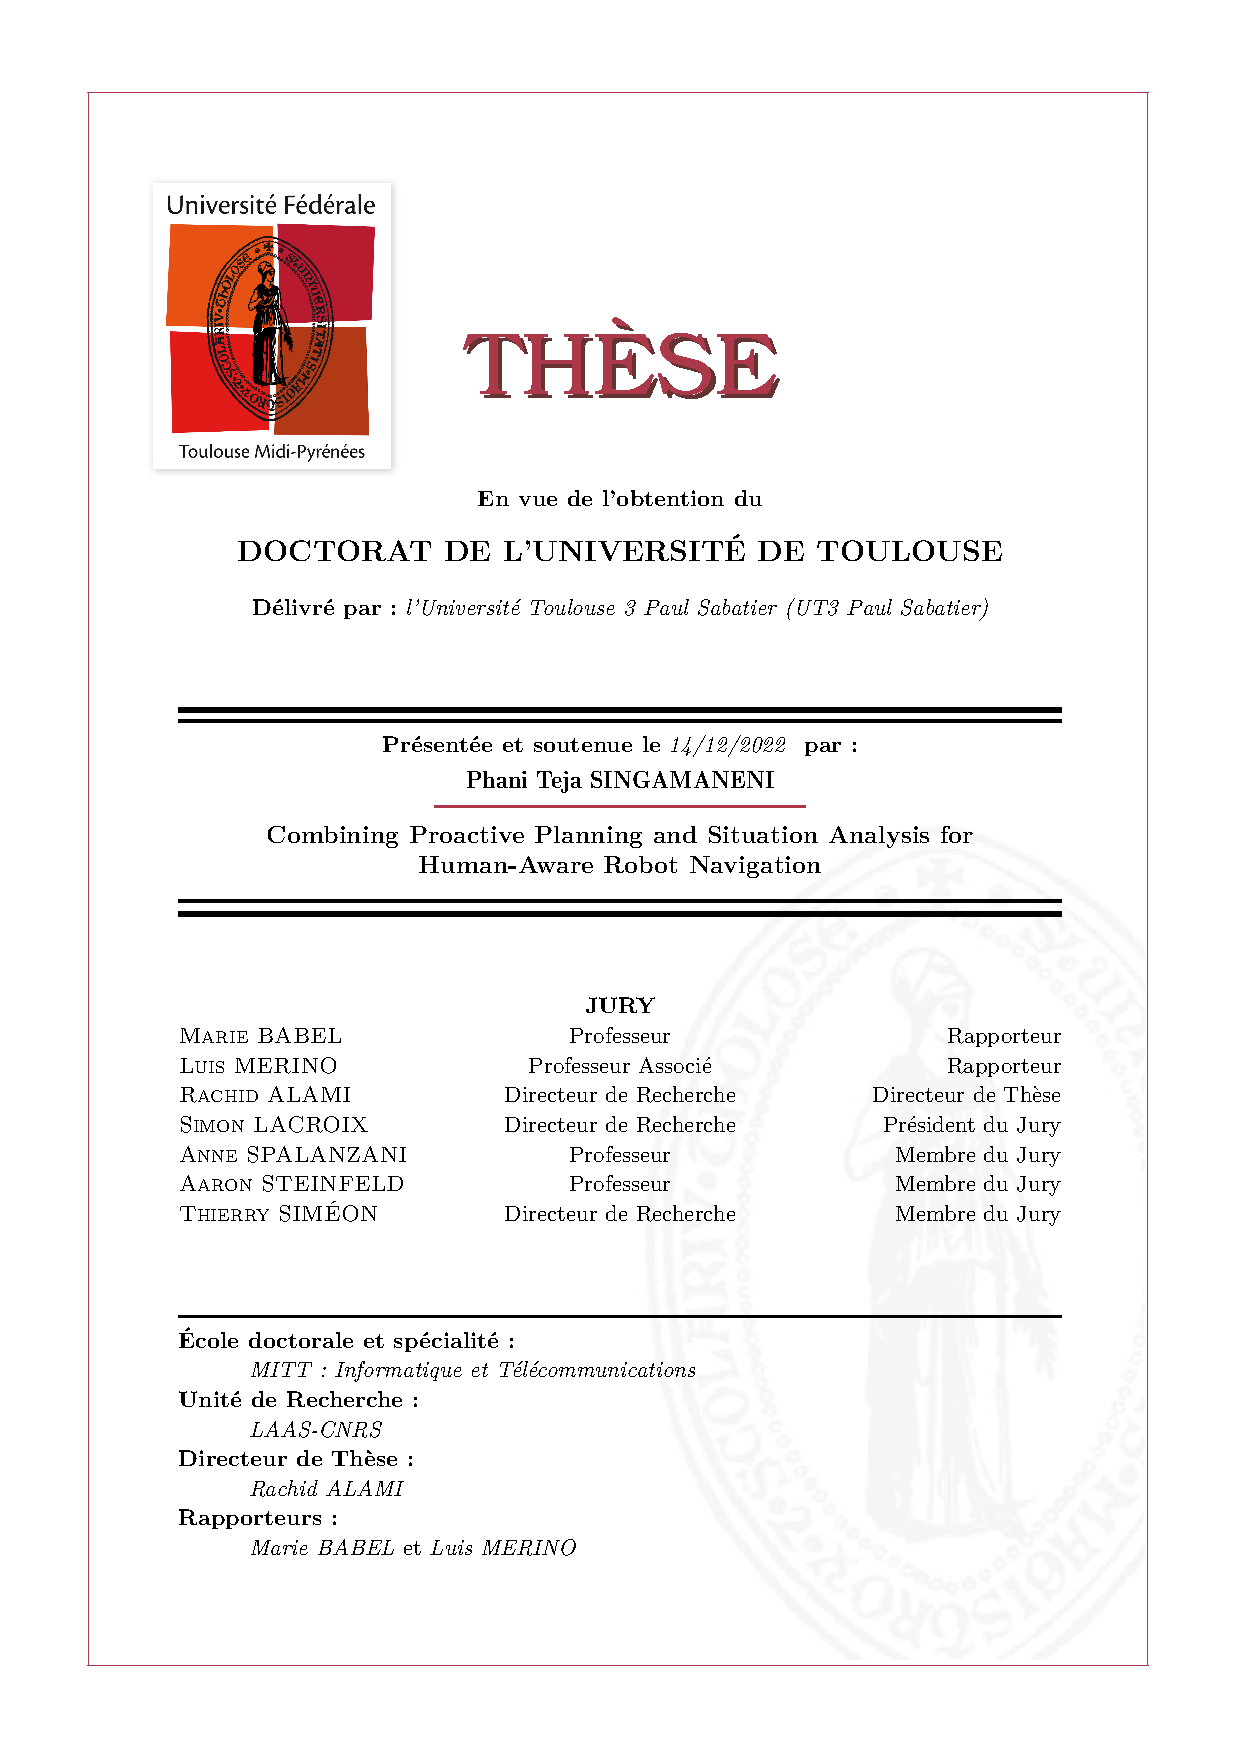
\includepdf[pages=-]{custom_cover_new.pdf}
%%%%%%%%%%%%%%% Uncomment this to use custom Cover page %%%%%%%%%


\cleardoublepage

\dominitoc

\pagenumbering{roman}

\cleardoublepage

%%%% Acknowledgments %%%%%
%%% Needs an update before and after the defence, write last
% \section*{Remerciemments}
 
blabla 

%%%% Abstract %%%%%
% \chapter*{Abstract}

% 4000 caractères

Although human-robot collaboration can be beneficial, most of today's robots work in spaces physically separated from humans, or their capabilities are severely limited in close proximity to humans. This work aims to bridge the gap between robotic capabilities and human expectations, fostering a new era of seamless and intuitive collaboration between humans and robots in shared environments to perform industrial, service or domestic tasks. More specifically, this manuscript presents a study of decision-making in the context of human-robot collaboration, particularly in the areas of task planning and simulating intelligent agents.

First, we discuss various fields and works related to human-robot collaboration to better understand my work's context. After an introduction to the HATP/EHDA task planner, I present my first contribution, which incorporates some concepts from the Theory Of Mind into task planning. Some models and algorithms are proposed and evaluated to better estimate and maintain human knowledge during collaboration, in order to better anticipate human behavior. As a result, we can identify when humans have false beliefs about a fact that is evaluated as relevant to the task. In this case, the robot can proactively inform the humans to correct the false information, or the robot can deliberately delay its actions so that the humans can see them. Our results show that this scheme effectively maintains human beliefs and solves a broader class of problems than HATP/EHDA, without communicating systematically.

My second contribution is a new approach to task planning producing a robot behavioral policy ensuring smooth collaboration where the human always has full decision latitude and the robot always conforms in parallel to these decisions. This approach is based on a concurrent and compliant joint action model we have designed. This model, in the form of an automaton, takes into account human uncontrollability and social cues. We also propose a new method of plan evaluation and selection based on the estimation of the human's internal preferences regarding the task. Empirical results show that this approach enables concurrent robot behavior that conforms to human's real-time decisions and preferences.

As another contribution validating the above approach, we implemented our proposed joint action model as an execution scheme into a dedicated simulator. Then, we conducted a user study where participants were invited to collaborate in several scenarios with a simulated robot following policies produced by our approach. In contrast with our approach, we used a baseline where the robot always imposes its decisions on the human. We showed through statistical analysis that our approach satisfies human preferences significantly more successfully than the baseline. Similarly, we have shown that our approach induces significantly more positive interaction, more adaptive and effective collaboration, and significantly more appropriate and accommodating robot decisions.

Finally, my last contributions concern simulating intelligent human agents. Such simulated agents endowed with decision-making capabilities can help to test, evaluate, and robustify interactive and collaborative robot systems. We propose a generic architecture to simulate an intelligent agent and present an implemented version for navigation use cases. An additional contribution capable of simulating several navigating agents is also presented.  

% \chapter*{Résumé}

Bien qu'il ait été montré que la collaboration humain-robot puisse être bénéfique, la plupart des robots actuels travaillent dans des espaces physiquement séparés de l'humain ou leurs capacités sont sévèrement limitées à proximité de l'humain. Ce travail vise à combler le fossé entre les capacités robotiques et les attentes humaines, en favorisant une nouvelle ère de collaboration transparente et intuitive entre les humains et les robots dans des environnements partagés pour réaliser à la fois des tâches industrielles, de services ou domestiques. Plus précisément, ce manuscrit présente une étude sur la prise de décision dans le contexte de la collaboration humain-robot, en particulier dans les domaines de la navigation et de la planification des tâches.

Tout d'abord, nous discutons de divers domaines et travaux en lien avec la collaboration humain-robot afin de mieux comprendre le contexte de mon travail. Après une familiarisation avec le planificateur de tâches HATP/EHDA, je présente ma première contribution qui incorpore certains concepts de la théorie de l'esprit dans la planification de tâches. Certains modèles et algorithmes sont proposés et évalués pour mieux estimer et maintenir les connaissances de l'humain lors d'une collaboration afin de mieux anticiper son comportement. En conséquence, nous pouvons identifier quand l'humain a une fausse connaissance d'un fait évalué comme pertinent pour la tâche. Dans ce cas, le robot peut informer l'humain de manière proactive pour corriger la fausse information ou le robot peut retarder volontairement ses actions afin qu'elles soient vu par l'humain. Les résultats montrent que ce schéma permet de maintenir efficacement les connaissances de l'humain et permet de résoudre une classe plus large de problèmes que HATP/EHDA tout en ne communiquant pas systématiquement.

Ma deuxième contribution est une nouvelle approche de planification des tâches produisant une politique comportementale du robot assurant une collaboration fluide où l'humain a toujours une latitude de décision totale et où le robot se conforme toujours en parallèle à ces décisions. Cette approche est basée sur un modèle d'action conjointe simultanée et accommodante que nous avons conçu. Ce modèle, sous la forme d'un automate, tient compte de l'incontrôlabilité de l'humain et des signaux sociaux. Nous proposons également une nouvelle méthode d'évaluation et de sélection des plans basée sur l'estimation des préférences internes de l'humain concernant la tâche. Les résultats empiriques montrent que cette approche permet un comportement concourant du robot qui se conforme aux décisions et aux préférences en temps réel de l'humain.

Pour valider l'approche précédente, nous avons mené une étude utilisateur à l'aide d'un simulateur spécialement développé à cet effet. Les participants ont été invités à collaborer dans plusieurs scénarios avec un robot simulé suivant les politiques produites par notre approche. Nous avons utilisé comme référence une approche opposée à la nôtre dans laquelle l'humain est forcé de se conformer aux choix du robot. Nous avons montré par une analyse statistique que notre approche permettait de satisfaire les préférences des humains de manière nettement plus satisfaisante. De même, nous avons montré que notre approche induit une interaction significativement plus positive, une collaboration plus adaptative et efficace, et des décisions du robot significativement plus adéquates et accommodantes.

Enfin, ma troisième contribution concerne la prise de décision dans le domaine de la navigation. Je propose un système simulant un avatar humain qui, en plus d'être réactif, prend des décisions rationnelles sur les tâches de navigation. Ce système sert d'outil de test et d'évaluation pour les systèmes de navigation robotique. Ainsi, ces derniers peuvent être évalués, ajustés et robustifiés en simulation pour réaliser plus rapidement des expériences matures dans la vie réelle.

\tableofcontents

% \printnomenclature
% \printnoidxglossary[type=\acronymtype]
% \listoffigures
% \listoftables
% Use \mtcfixnomenclature below if you have a glossary (added with
% \printnomenclature above) and you're see a shift in the mini-table of
% contents at the begining of each chapter (example: no mini-toc in chapter 1;
% mini-toc of chapter 1 appearing in chapter 2; and so on).
%
% You should not use \mtcfixnomenclature if you have no glossary (that means,
% if you don't use \printnomenclature or if your glossary is empty).
%\mtcfixnomenclature

\mainmatter
% \chapter*{Introduction}
\addstarredchapter{Introduction}
\markboth{Introduction}{Introduction}

\newcommand{\mysection}[1]{%
    \section*{#1}%
    \addcontentsline{toc}{section}{#1}%
    \markright{#1}%
}


\minitoc

\acrfull{hrc} is a growing field in robotics and \acrfull{ai} research that aims to enable safe and effective teamwork between humans and robots.
This field mostly concerns fully autonomous robots. Hence, for instance, it excludes exoskeletons or teleoperated robots such as surgery manipulators or remotely operated (aerial) vehicles. 

In this manuscript, robots are considered autonomous tools able to interact physically with their environment. As tools, robots should facilitate human tasks by reducing both the required physical effort and mental workload. 
Industrial robots are already popular in factories because they are fast, accurate, reliable, and never tire, which makes them ideal for repetitive factory tasks. 
However, such robots are usually contained in dedicated areas where humans cannot enter for safety reasons. 
Hence, it is still an open challenge to endow robots with enough reliable reasoning capabilities and compliant motion control to allow efficient and trusted direct collaboration between humans and robots. 

This work aims to design autonomous robots able to make explainable, acceptable, and efficient decisions to collaborate with humans. Moreover, \acrshort{hrc} can also occur in various contexts that must be taken into account which range from co-worker robots in factories to householder robots for our everyday lives and include service robots in public places like restaurants and shops.


\mysection{Human-Robot Collaboration Challenges}

\acrshort{hrc} opens several challenges to address, each corresponding to a different aspect or functionality that the robot should be endowed with to fulfill its role. Hence, the ideal general collaborative robot should be the aggregation of all the notions below: 

\begin{itemize}
    \item \textbf{Navigation}: The robot should be able to acceptably and efficiently move in a human-populated environment. This implies being mechanically designed for it, anticipating and planning correct trajectories, and being able to adapt and follow these trajectories in real time. The robot should not move threateningly and should account for humans.

    \item \textbf{Manipulation}: The robot should be able to manipulate objects to interact with its environment. Hence, the robot should have an actuator like an arm and a gripper and should be able to exhibit motions that are efficient and safe to nearby humans.

    \item \textbf{Decision-making}: The robot should be able to make relevant decisions to be collaborative. This implies being able to plan its actions to solve a collaborative task. It also implies being able to supervise the task execution and make online decisions to adapt to uncertainties in real time, which includes human actions and commands. 

    \item \textbf{Communication}: To achieve congruent interaction and collaboration, collaborative agents must communicate. This implies that the robot should be able to communicate information to the human and understand the one received from the latter. These communications can be of various types, e.g., verbal, using natural language, prompting text on a screen, and signaling through robot movements (arms, head, mobile base). More innovative techniques can also be mentioned such as projecting arrows or desired paths on the ground, and using Augmented Reality to show internal information on the robot (decision, next action, etc...).

    \item \textbf{Perception}: Eventually, the robot must be able to perceive its environment. This is mandatory for the robot to have a reliable perception scheme to know the position of near objects, obstacles, and humans. First, relevant sensors must be used and placed on the robot or in the environment itself. After, from sensory data, some analysis and reasoning processes must extract relevant facts about the robot's environment such as objects' positions, spatial relations, reachable objects, human knowledge and intentions, the state of the current goal, and more. This constitutes the knowledge of the robot which may include an estimation of the near human knowledge. Perception is critical because most of the other challenges rely on the robot's knowledge.

\end{itemize}
    

\mysection{Contributions and manuscript organization}

The main challenge of HRC/HRI addressed in my PhD is decision-making. My work led to three main contributions concerning two distinguishable subfields. My two first contributions concern decision-making during task planning, to decide and plan the robot's action in order to solve a task collaboratively or simply in the presence of humans. My third contribution addresses decision-making in navigation, especially, how to simulate interactive social navigating agents endowed with decision-making processes to challenge robot navigation schemes.
As a result, the structure of my manuscript is as follows.

Chapter~\ref{chap:1} provides more details about the context of my PhD by discussing related fields and works of HRC. This chapter eventually highlights the gap in the literature that motivates my PhD work.

Part~\ref{part:1} gathers all my work concerning task planning for HRC. It represents a major portion of my PhD work and includes the chapters~\ref{chap:2}, \ref{chap:3}, \ref{chap:4}, \ref{chap:5}, and \ref{chap:6}.

Chapter~\ref{chap:2} familiarizes the reader with the HATP/EHDA task planner. Indeed, I participated in its development and this planner has been the keystone of my two contributions to task-planning for HRC. Hence, the reader should understand both this task planner's motivation and methods.

Chapter~\ref{chap:3} introduces my first main contribution which incorporates Theory of Mind concepts in HRC task-planning, more precisely, in the HATP/EHDA planning process.
Some models and algorithms are proposed and evaluated to better estimate human beliefs in order to better anticipate their potential actions. As a result, we can identify when the human has a false belief about a fact evaluated as relevant for the task. In such cases, the robot can proactively inform the human to correct the false belief or the robot can purposely delay its action to make sure the human sees its execution and infer the corresponding fact, avoiding verbal communication. 

In Chapter~\ref{chap:4}, as my second main contribution, I address the lack of concurrent actions of HATP/EHDA to improve fluency in collaboration. Inspired by the Joint Action literature, we designed a model of concurrent and compliant execution for HRC in the form of an automaton. We also propose to evaluate plans based on an estimation of the human inner preferences. A novel task planning approach taking into account the mentioned execution model and plan evaluation is proposed. This approach generates concurrent robot policies compliant with human online decisions and preferences. 

Chapter~\ref{chap:5} is a technical description of an interactive simulator I developed to execute the robot policy generated by the approach described in the previous chapter. This simulator proposes an execution scheme based on the model of execution to run and supervise the robot policy in a 3D simulator. It also allows a human operator to perform actions through intuitive mouse control. Hence, this simulator offers a way to collaborate with a robot following the approach we designed and is used in the next chapter to evaluate the approach.    

Chapter~\ref{chap:6} presents a user study validating the approach proposed in Chapter~\ref{chap:4} using the simulator described in Chapter~\ref{chap:5}. For this purpose, several scenarios have been designed using a BlocksWorld task, and human participants were asked to collaborate with the simulated robot to evaluate its behavior. We compared our approach with a baseline consisting of a robot following a simpler version of the model of execution. 

Conclusions regarding part~\ref{part:1} follow this chapter before starting the second part of this thesis. 

Part~\ref{part:2} concerns decision-making in navigation and how to simulate interactive social navigating agents. Despite not being my main research topic, this subject represents significant work in my PhD. This part includes the two last chapters: \ref{chap:7} and \ref{chap:8}.

Chapter~\ref{chap:7} describes my third contribution in which I address the decision-making challenge in navigation to allow the robot to move in a human-populated environment acceptably and efficiently. I developed a system producing an ``intelligent'' human avatar that, while being reactive, can make rational decisions about navigation tasks. This system serves as a benchmarking and testing tool for robot navigation systems to be challenged. This way, robot navigation systems can be evaluated, tuned, and stress tested in simulation allowing them to run mature real-life experiments faster.  

Chapter~\ref{chap:8} presents an additional work with the same rationales as the approach described in Chapter~\ref{chap:7} and is largely inspired by it. However, this work addresses a major limitation of the previous one which is not being able to simulate several human agents. This other approach can choreograph several agents with group movements and social behaviors. Despite having limited individual decision-making compared to the previous approach, this additional work generates pertinent and challenging intricate situations with several agents which is beneficial to the social robotic research.

Conclusions concerning both Chapter \ref{chap:7} and \ref{chap:8} end part~\ref{part:2}.

Eventually, I share general conclusions regarding all of my PhD work in a dedicated part before providing additional materials in the appendix.  

\mysection{List of Publications}

\subsubsection*{As main author}
\begin{itemize}

    \item Anthony Favier, Phani-Teja Singamaneni, Rachid Alami. Simulating Intelligent Human Agents for Intricate Social Robot Navigation. Social Robot Navigation workshop - Robotics: Science and Systems (RSS'21), Jul 2021, Washington, United States. 
    \item Anthony Favier, Phani-Teja Singamaneni, Rachid Alami. An Intelligent Human Avatar to Debug and Challenge Human-aware Robot Navigation Systems. Late Breaking Report - 2022 ACM/IEEE International Conference on Human-Robot Interaction (HRI'22), Mar 2022, Sapporo, Japan. 
    \item Anthony Favier, Shashank Shekhar, Rachid Alami. Robust Planning for Human-Robot Joint Tasks with Explicit Reasoning on Human Mental State. AI-HRI Symposium at AAAI Fall Symposium Series (FSS'22), Nov 2022, Arlington, United States. 
    \item Anthony Favier, Shashank Shekhar, Rachid Alami. Anticipating False Beliefs and Planning Pertinent Reactions in Human-Aware Task Planning with Models of Theory of Mind. PlanRob Workshop - International Conference on Automated Planning and Scheduling (ICAPS'23), Jul 2023, Prague, Czech Republic. 
    \item Anthony Favier, Shashank Shekhar, Rachid Alami. Models and Algorithms for Human-Aware Task Planning with Integrated Theory of Mind. IEEE International Conference on Robot and Human Interactive Communication (RO-MAN'23), Aug 2023, Busan, South Korea. 
    \item Anthony Favier, Phani Teja Singamaneni, Rachid Alami. Challenging Human-Aware Robot Navigation with an Intelligent Human Simulation System. Social Simulation Conference (SSC'23), Sep 2023, Glasgow, France. 
    \item Anthony Favier, Rachid Alami. Planning Concurrent Actions and Decisions in Human-Robot Joint Action Context. Symbiotic Society with Avatars workshop - ACM/IEEE International Conference on Human-Robot Interaction (HRI'24), Mar 2024, Boulder, United States.

\end{itemize}
    
\subsubsection*{As co-author}
\begin{itemize}
    
    \item Guilhem Buisan, Anthony Favier, Amandine Mayima, Rachid Alami. HATP/EHDA: A Robot Task Planner Anticipating and Eliciting Human Decisions and Actions. IEEE International Conference On Robotics and Automation (ICRA 2022), May 2022, Philadelphia, United States. ⟨10.1109/ICRA46639.2022.9812227⟩. 
    
    \item Phani-Teja Singamaneni, Anthony Favier, Rachid Alami. Towards Benchmarking Human-Aware Social Robot Navigation: A New Perspective and Metrics. IEEE International Conference on Robot and Human Interactive Communication (RO-MAN), 2023, Aug 2023, Busan, South Korea.
    \item Phani-Teja Singamaneni, Anthony Favier, Rachid Alami. Human-Aware Navigation Planner for Diverse Human-Robot Contexts. 2021 IEEE/RSJ International Conference on Intelligent Robots and Systems (IROS), Sep 2021, Prague (online), Czech Republic. 
    \item Phani-Teja Singamaneni, Anthony Favier, Rachid Alami. Invisible Humans in Human-aware Robot Navigation. IEEE International Conference on Robotics and Automation (ICRA 2022), May 2022, Philadelphia, United States.
    \item Phani-Teja Singamaneni, Anthony Favier, Rachid Alami. Watch out! There may be a Human. Addressing Invisible Humans in Social Navigation. 2022 IEEE/RSJ International Conference on Intelligent Robots and Systems (IROS 2022), Oct 2022, Kyoto, Japan. 

    \item Olivier Hauterville, Camino Fernández, Phani-Teja Singamaneni, Anthony Favier, Vicente Matellán, et al.. IMHuS: Intelligent Multi-Human Simulator. IROS2022 Workshop: Artificial Intelligence for Social Robots Interacting with Humans in the Real World, Oct 2022, Kyoto, Japan. 
    \item Olivier Hauterville, Camino Fernández, Phani-Teja Singamaneni, Anthony Favier, Vicente Matellán, et al.. Interactive Social Agents Simulation Tool for Designing Choreographies for Human-Robot-Interaction Research. ROBOT2022: Fifth Iberian Robotics Conference, Nov 2022, Zaragoza, Spain. 
\end{itemize}
    
    
    
% \ifdefined\included
\else
\setcounter{chapter}{0}
\dominitoc
\faketableofcontents
\fi

\chapter{Task Planning for Human Robot Collaboration Context}
\chaptermark{Task Planning for Human Robot Collaboration Context}
\label{chap:1}
\minitoc

\section{Task Planning}

\subsection{Various techniques}
\subsection{Offline}
\subsection{Online}

\section{HRI Interaction}

\subsection{human human interaction}
\subsection{human computer interaction}
\subsection{human robot interaction}

\subsection{navigation}
\subsection{dialogue}


\section{HRC Collaboration}

\subsection{joint action}
\subsection{Whole architecture to work}
\subsection{execution policy, leader follower?}

\section{Background and Our Approach}
\subsection{human-aware task planning state of the art}
\subsection{our Approach}



% \ifdefined\included
\else
\setcounter{chapter}{1} %% Numéro du chapitre précédent ;)
\dominitoc
\faketableofcontents
\fi

\chapter{A Human-Aware Task Planner Emulating Human Decisions and Actions (HATP/EHDA)}
\chaptermark{HATP/EHDA}
\label{chap:2}
\minitoc

\chapabstract{This chapter presents the HATP/EHDA task planner. This planner has been the keystone of most of my work. Hence, the reader should understand the motivation and methods of this task planner.}

\section{Introduction}

I was introduced to task planning with the work of a PhD student from my lab, Guilhem Buisan. I slightly contributed to the original version and then proposed two extensions of his work. However, Guilhem mainly designed and implemented this novel \textbf{H}uman-\textbf{A}ware \textbf{T}ask \textbf{P}lanning approach dedicated to \acrfull{hri}, which plans the robot's actions while estimating and \textbf{E}mulating the \textbf{H}uman \textbf{D}ecisions and \textbf{A}ctions, namely \textbf{HATP/EHDA}. 

We believe this planning approach suits the needs of \acrshort{hri} scenarios well; thus, it became a laboratory to address relevant challenges of task planning for \acrshort{hrc}. 
Two of my main contributions include addressing such challenges and implementing the solutions as extensions of HATP/EHDA.   
Consequently, it is essential to understand this work's motivation and methods well before introducing my proper contributions. This section introduces, motivates, and explains the HATP/EHDA approach as a background to the other chapters. 
A detailed description of this prototypical planner is already given in Buisan's thesis~\cite{thesisBuisan21}. Thus, large parts of this section are directly retrieved from Buisan's thesis, but they are essential to have in mind. Some notations are adapted to match the descriptions of my contributions in the following chapters. 

\section{A Hierarchical Agent-Based Task Planner (HATP)}

My work and HATP/EHDA are part of a line of work that started with the \acrfull{hatp} \cite{alili2009task,lallement2014hatp}.

Based on \acrfull{htn}, this planner can elaborate a multi-agent plan based on a single HTN tree. Moreover, it maintains one belief base per agent, allowing the writer to write task decomposition rules and action preconditions and effects in any agent belief base. This approach produces a joint plan that includes actions from all involved agents. 

Finally, to make \acrshort{hatp} suitable to \acrshort{hri} scenarios, specific mechanisms to compute costs and filter plans have been included. To this end, \acrshort{hatp} allows balancing efficiency, wasted time, agent effort, intricacy, and undesirable states or sequences. This way, social rules can be defined to produce a collaborative plan that humans will likely accept. 

However, \acrshort{hatp} assumes a shared goal has been established between humans and robots before planning. The generated plan will be shared with and accepted by humans before execution. Indeed, HATP does not represent humans as agents having separate decision-making processes that may lead to diverging plans without robot communication. Hence, any human deviation from their generated stream of action needs supervision to perform repair action or request a replanning. Such an approach can work well, but it assumes that communication can easily be done at any point in the plan. However, this assumption is not always verified for various reasons, \textit{e.g.} noisy environments, making communication costly.
Additionally, any human deviation, \textit{e.g.} due to inattention, will put the robot in a failure state, which needs to be fixed before continuing (replanning).

\section{Rationales of the HATP/EHDA Approach}

The \acrshort{hatp} approach produces what is estimated to be the best joint plan for solving the task. Hence, this approach assumes that humans will likely accept and follow the produced plan. This approach leaves no room for online human decisions and assumes a fully committed human through a previously established shared goal. This approach also considers one shared task representation and knowledge base. To cater to the limitations of \acrshort{hatp}, I participated in the development of a new approach, HATP/EHDA, which tries to satisfy several objectives: 
\begin{enumerate}
    \item \textbf{Plan without assuming a prior shared goal.} In \acrshort{hri} scenarios, the robot and the human do not always share a goal. The robot can, for example, plan to perform a task around humans that are not involved at first, or it may be requested by a human to do a task without wanting to take part in it. HATP/EHDA can balance between integrating the sharing of a goal with a human (assumed to be collaborative) in the plan and making the robot do the task alone or integrating the eventuality to ask for punctual human help. 

    \item \textbf{Model the human decision processes.} When taking part in a task, a human (assumed willing to collaborate with the robot) will also plan to reach their (potentially shared) goal. HATP/EHDA must be able to account for this to provide plans that are expected and explainable by the human partner.

    \item \textbf{Help the human decisions, but not compel them.} Unlike \acrshort{hatp}, HATP/EHDA should account for human decision-making flexibility. While modeling the human decision processes, it is possible to narrow down the possible human actions, and the generated plans must help the supervision (execution of the plan) avoid replanning or repairing during the execution by considering several human actions.

    \item \textbf{Model the potential human reactions.} It is possible to predict that the human may react to some situations, interrupting or helping their current task. Two causes have been identified for these reactions. First, they can result from specific world states humans perceive and interpret. Then, they can also originate from explicit communications issued by the robot. These communications can either be a belief alignment, updating the human knowledge and impacting their decisions, a request to perform a specific action, or a request to help the robot with a shared goal, needing the human to plan for it.

    \item \textbf{Act and decide on the different agents' beliefs.} It is crucial to be able to represent actions as having different effects on the beliefs of the robot or the human. Indeed, some robot actions are partially or not observable by humans; humans cannot know the complete new world state when performing them. Besides, these effects and their observability often depend on the current world state, whose representation must be supported by the planner. Then, planning decisions may require reasoning on both the robot's and human's beliefs. This is especially true with communication actions aiming to align knowledge or ask questions. Finally, some actions of pure decision have no direct effect on the world but only on the internal beliefs of the agents. For example, observation actions will only update the beliefs of the agent doing it.

    \item \textbf{Decide not only on the world state but also on the decision processes of the agents.} Some decisions made during the planning process require access to the agents' beliefs representing the world state and the estimation of their planning processes. For example, the decomposition of a task by the robot may be impossible if some other task is already performed in its partial plan. Other decisions may also need the estimation of the current human planning process. For example, if it were estimated earlier in the plan that the human would perform a specific task decomposition, the planner would assign a complementary task to the robot.

    \item \textbf{Adapt to the human experience, trust, and preferences.} We also want the planning process to be adjusted depending on the actual human it is planning with. It must perform its planned search differently, whether the human has the habit of performing this particular task with the robot or not. Moreover, the human model can be adjusted to the human's trust in the robot and their preferences.

\end{enumerate}

\section{Related work} \label{sec:ch2_related_work}

An approach to solving a collaborative task is to produce a joint plan that includes coordinated robot and human actions. This plan must be shared, accepted, and followed to solve collaboratively the common goal. This approach is used in the \acrshort{hatp} planner presented above. By assuming the plan must be followed, the human cannot deviate from the generated plan. Hence, this approach assumes that the human is controllable. 
In \cite{johannsmeier2016hierarchical}, the authors use the same assumption and propose a task allocation framework for human-robot collaborative assembly line tasks. They propose representing the task through an AND/OR graph and solving the optimal sub-task allocation problem considering a given cost function. Action sequences are extracted from this allocation and then shared with the respective agents to be executed. Hierarchical and concurrent hybrid state machines handle the execution of these sequences. This copes with unpredictable events likely to happen in dynamic and partially known environments, especially in the presence of humans.  

Additionally, some works are focused on \acrshort{hrc}'s psychological aspect, like the plan's acceptability and explainability. This is beneficial to the approach described just above. In \cite{chakraborti_plan_2017}, the authors propose to improve the explainability of a robot plan by using both a robot model $\mathcal{M^R}$ and the estimation of the model the human has of it $\mathcal{M}^R_h$. This approach, called model reconciliation, aims to make identical the optimal plans generated using both models, i.e., $\mathcal{M^R}$ and $\mathcal{M^R_h}$. They define a list of operators to modify the different models until the plans match. 
Although this approach interestingly improves the explainability of the robot's plan, it does not consider the two agents to collaborate directly. Indeed, the plan produced only contains robot actions. 

Producing a joint plan that considers the human controllable is efficient and acceptable in industrial contexts. Indeed, the human is working and thus highly committed and focused on the task. Even if humans appreciate flexibility, in this context, their priority is instead task efficiency.
However, this assumption can become burdensome for humans in other contexts, such as household ones, where humans are likely to be distracted, change their minds, and tend to prioritize minimizing their effort and flexibility instead of task efficiency. 

As a result, some approaches started to consider a distinct human model $\mathcal{M}^R_h$ to plan the robot action.
A first approach, described in \cite{hoffman_effects_2007}, proposes an adaptive action selection mechanism for a robotic teammate, making anticipatory decisions based on the confidence of their validity and their relative risk. They demonstrate improved task efficiency and fluency compared to a purely reactive process. The human behavior is modeled with a First-Order Markov Process and learned through Bayesian estimate. The probabilities constituting the human model are used in the cost evaluation of different plans, eventually leading to a robot action selection, producing an adaptive and proactive robot plan. 
In \cite{unhelkar2020decision} is proposed an approach based on \acrfull{pomdp} called CommPlan. The \acrshort{pomdp} is built using a user-defined \acrfull{mdp} representing the collaborative task and an \acrfull{amm} representing the human decision-making process. Solving this \acrshort{pomdp} produces a robot policy that decides when the robot has to communicate about its beliefs, when to question the human about theirs, and when to ask the human to perform an action. Besides, the \acrshort{amm} is not only specified by an expert modeler but also refined during the interaction via learning. However, the approach considers the human model as an oracle on which reasoning is hardly possible.

Other works extend the use of a distinct human model to explicitly predict and anticipate the actions the human is likely to perform. Then, for each possible human action, the best robot's actions are determined to account for human unpredictability. This is the approach used in HATP/EHDA.
This other work \cite{buckingham_robot_2020} also uses this approach. They propose a unified scheme to cope with collaborative, adversarial, and non-involved human agents. This scheme considers given mental models for each human co-present with the robot, which might interact with the latter. These mental models are queried to estimate a set of actions each agent is likely to perform given a state. The robot's actions are planned according to these estimated actions to reach the robot's goal and potentially achieve the human agents' goal. In doing so, the robot's actions can influence the human ones without explicit communication, helping the robot achieve its goal. HATP/EHDA similarly queries a human mental model and uses an AND/OR graph where OR nodes represent possible robot actions in a state and AND nodes represent the possible human actions estimated by the models. However, despite saying the model can be generic, this work uses a basic breadth-first search planner to produce a set of minimal-cost plans solving the estimated human goal. Then, they extract the first actions of each plan to produce a set of actions the human is likely to perform. No details are given on the cost evaluation. This approach does not seem to consider human actions that are sub-optimal but still probable, which can be due to inattention. Moreover, the robot actions are selected by using a Min-Max approach on the AND/OR graph, minimizing the worst-case. This approach works well in adversarial setups and still allows cooperative human interventions. However, it is unclear how these cooperative actions are taken into account in the robot decision process. Assuming that the human will be adversarial, the robot might make ``wrong'' decisions, possibly preventing an efficient and optimal cooperative execution. HATP/EHDA minimizes the average cost of all possible human decisions, optimizing uniformly for any human decisions. This approach considers humans congruent, rational, and cooperative but not necessarily involved in the robot's task. Hence, HATP/EHDA does not account for adversarial humans but addresses the other cooperation types better.
\cite{koppula2016anticipatory} also explicitly estimated the most likely human actions to generate the robot policy, but they use a probabilistic and learning approach. They propose a two agent collaborative \acrshort{mdp} model and learn robot policies by taking into account the actions that can be performed by the human. They represent the environment in terms of the object affordances and learn the activity model from RGB-D videos of a human performing the activities. Then, they use this learned task model in a distributed Q-learning algorithm to learn the robot policy for a given new environment. 
The human capabilities are captured in a \acrshort{mdp}. Thus, the possible human actions are estimated by balancing the human habits and the best ($\epsilon$-optimal) action given by the \acrshort{mdp}. 


Another line of work, sometimes also using human models, is focused on online and reactive planning. The robot's behavior is decided online using planning techniques but on limited horizons. This produces robot behaviors that are adaptive to human decisions and potentially unexpected environmental changes and events. However, due to the limited horizon to maintain a real-time reactive behavior, the robot behavior's optimality is not guaranteed and might lead to dead ends. Nevertheless, these online approaches usually robustify the robot's behavior and are reactive to failures. Therefore, they could/should complement offline planning approaches like HATP/EHDA.
The two-sided work \cite{sanelli_short_term_2017} is in this line of work. First, they propose a conditional planning system that considers uncertainties, primarily due to human agents. This planning approach is based on planner Contingent-FF \cite{hoffmann2005contingent}. Then, they propose a component to translate these plans into a Robust Petri-Net Plan (PNP) to handle their execution. This translation is inspired by work \cite{iocchi2016practical}, which improves plans with execution rules. Eventually, these plans are executed with an existing module called PNPRos \cite{ziparo2011petri}. Interestingly, the expected human actions are transformed into sub-Petri Nets where the robot elicits the action (\textit{e.g.}, via verbal communication) if the human does not perform it by themselves. 
However, this approach does not model either reason on a distinct human agent model. Hence, the human reasoning process, goal, and belief are not modeled. This means that the interaction is limited to requesting the human to perform single actions without setting a proper high-level joint goal. This can be efficient in some situations, like a service robot providing information and requesting answers to some questions, such as the examples presented by the authors. However, repeated punctual interventions to perform a more extended task collaboratively can become unpleasant for the human.
In \cite{DarvishSMC21}, they propose a hierarchical human-robot cooperation architecture called FlexHRC+ designed to provide collaborative robots with an extended degree of autonomy when supporting human operators in high-variability shop-floor tasks. This online architecture is organized into three levels: perception, representation, and action, producing robust, adaptive, and sometimes proactive collaboration. 
They use hierarchical AND/OR graphs where arcs are sub AND/OR graphs to reduce the complexity of task descriptions, especially when including repetitive subsequences of action (like mounting four table legs). This representation is close to the \acrshort{htn} one used in HATP/EHDA. 
A reactive human-aware task planner is proposed in \cite{fusaro_human_aware_2021}, taking advantage of the Behavior Tree paradigm. The approach plans the robot's actions online by minimizing weighted costs based on duration, ergonomics, and distance, which are updated online. Therefore, the robot can adapt to dynamic changes in the environment and to human intentions, motions, decisions, and availability. This approach permits considering different levels of engagement between robots and humans: coexistence, cooperation, and autonomous task execution. 

Finally, in \cite{izquierdo_badiola_improved_2022}, the authors combine the production of a joint plan to solve a common goal with the reactive aspect of previous approaches. 
They use a so-called ``\textit{agent state}'' to model the human mental state and translate it into action costs in a PDDL domain. This model comprises the \textit{Capacity} evaluating if the human is capable of performing an action at the specified location without difficulty, the \textit{Knowledge} evaluating if the human has all necessary knowledge to perform their assigned actions, and the \textit{Motivation} indicating if the agent is committed towards the common goal, active and not distracted. 
In their approach, the \textit{agent state} is sensed and updated during execution. Then, whenever changes in the \textit{agent state} are detected, a replan is triggered to consider those changes in the plan, often inducing a reassignment of the actions and avoiding the probable failure of the initial plan. However, the authors do not provide a method to effectively sense and estimate the \textit{agent state} but prove its usefulness by simulating its acquisition.


\section{Running Example}

\begin{figure}
    \centering
    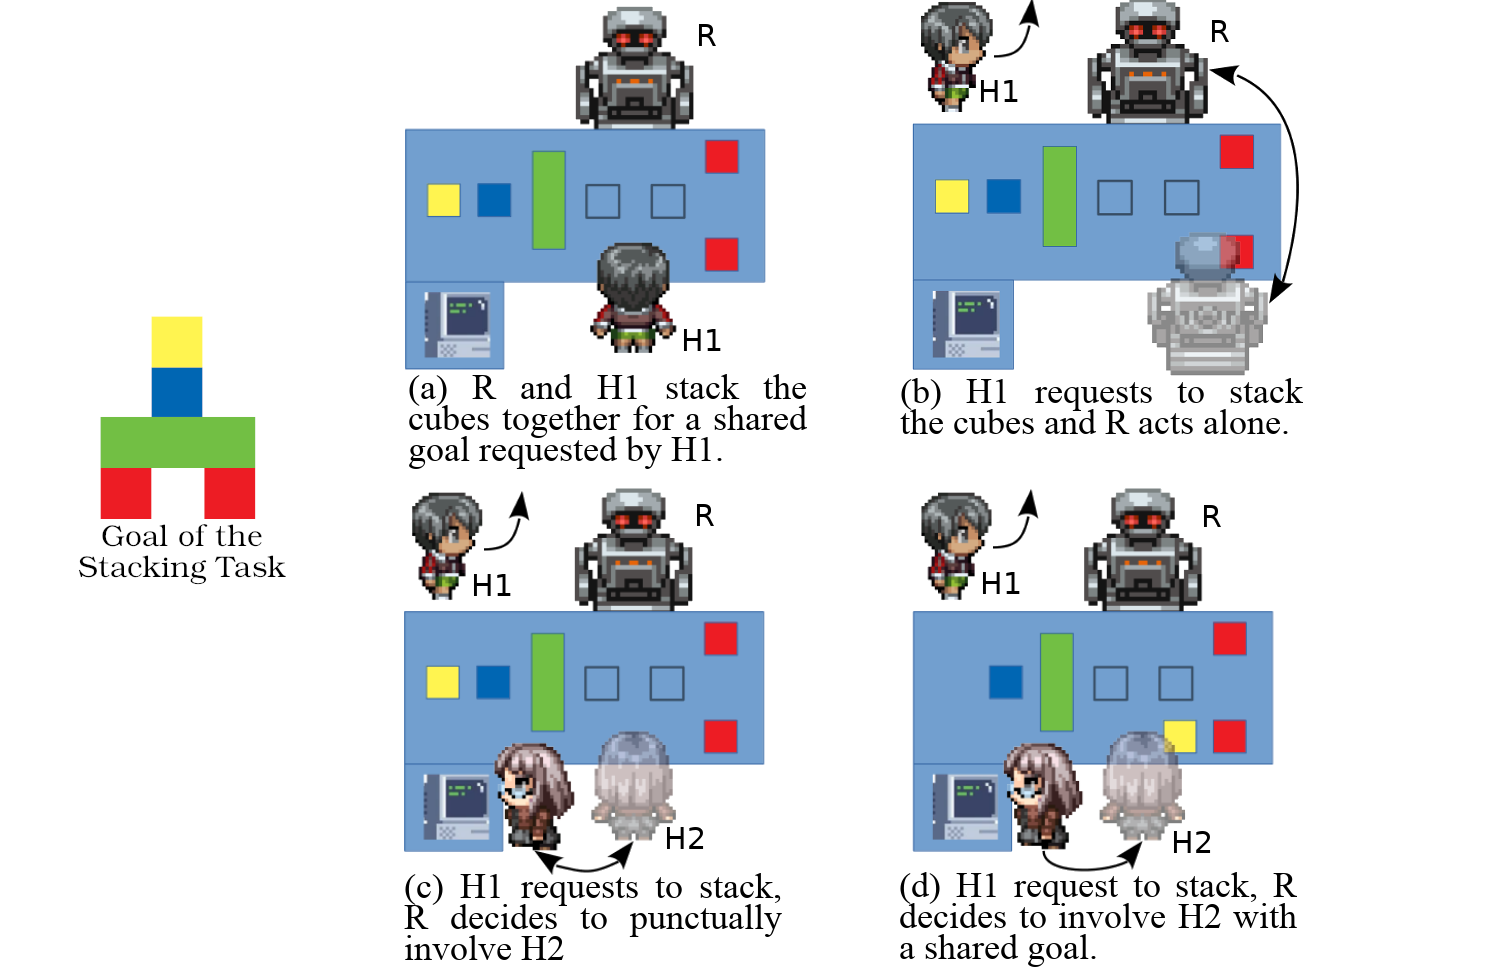
\includegraphics[width=\linewidth]{Chapter2/scenarios.png}
    \caption{Cube stacking scene: A different plan is selected for each scenario, involving nearby humans in the least disturbing way possible}.
    \label{fig:scenarios}
\end{figure}

To highlight the potential of our approach, we present a cube-stacking scene as an example. The scene is depicted in four different scenarios in \ref{fig:scenarios}. The goal consists of stacking the colored cubes on the empty marks to match the colors on the figure's left. All cubes placed in the middle of the table are reachable from anywhere. However, when close to one side, a cube is only reachable from this specific side. Notice that one of the required red cubes is located on the opposite side of the table and cannot be grabbed by the robot in the initial state.

A first human, called \textit{H1}, requests the robot to stack the colored cubes to match the goal pattern given. In the first case (a), \textit{H1} set a shared collaboration goal by requesting the robot to stack the cubes together with them. However, \textit{H1} can also just give their request to the robot and leave. In such a case, the robot has three possibilities. First, in (b), the robot can solve the task alone but must move to the other side of the table, which is slow and costly. Secondly, in (c), the robot can ask another nearby human, \textit{H2}, for punctual help with the unreachable red cube. \textit{H2}'s reaction can be to put the red cube directly in the stack or only make it reachable to the robot. Finally, the robot can set a shared goal by requesting \textit{H2} to help it build the stack together. 

The HATP/EHDA approach explores and evaluates all these kinds of scenarios to produce the robot policy.


\section{Formalization}

This section describes the formalization introduced by the HATP/EHDA planning approach and used or adapted in my contributions. It includes descriptions of the problem specifications and the solution produced by the planner.  

\subsection*{Problem Specification}
\label{sec:problem_spec}

The notations from Buisan's thesis have been adapted to match the notations in this thesis and ease readers' comprehension. We start from the classical planning formalization described in~\cite{ghallab2016automated}.

\begin{definition}
    \textbf{(Classical Planning Domain $\Sigma$.)} A \emph{classical planning domain} is a state-transition system in the following form: $\Sigma = (S, A,\gamma)$. $S$ is a finite set of \emph{states} in which the system may be, $A$ is a finite set of \emph{actions} that the agents may perform, $\gamma: S \times A \rightarrow S$ is a \emph{state-transition function}. Each \emph{state} $s \in S$ is a description of the properties of various objects in the planner's environment. 
    \label{def:classical_planning_domain}
\end{definition}

To represent the objects and their properties, we will use two sets $B$ and $X$: $B$ is a set of names for all the objects, plus any mathematical constants representing the properties of those objects. $X$ is a set of syntactic terms called state variables, s.t. the value of each $x \in X$ depends solely on the state $s$.

\begin{definition}
    \textbf{(State-variable $x$.)} A \emph{state-variable} over $B$ is a syntactic term $x = sv(b_1, ..., b_k)$, where $sv$ is a symbol called the state variable's name, and each $b_i$ is a member of $B$ and a parameter of $x$. Each \emph{state-variable} $x$ has a range, $\textit{Range}(x) \subseteq B$, which is the set of all possible values for $x$.
    \label{def:state_variable}
\end{definition}



Here is the description of the sets $B$ and $X$ for the stacking example given in the introduction:
{\small
\begin{align*}
&B           = Entities \cup Locations \cup Reachability \cup Booleans \cup \{\textsf{nil}\} \\
&\quad Entities    = Agents \cup Cubes\\
&\quad Agents      = \{ \textsf{R}, \textsf{H} \} ~~ \backslash\backslash~\textsf{R}:robot,~\textsf{H}:human\\
&\quad Cubes     = \{ \textsf{red1}, \textsf{red2}, \textsf{green1}, \textsf{blue1}, \textsf{yellow1} \}\\
&\quad Locations     = \{ \textsf{base1}, \textsf{base2}, \textsf{bridge}, \textsf{top1}, \textsf{top2} \}\\
&\quad Reachability     = \{ \textsf{middle}, \textsf{side\_h}, \textsf{side\_r} \}\\
&\quad Booleans    = \{ \textsf{true},\textsf{false} \}\\
&\\
&X = \{ at(e), holding(a), solution(l) ~ | ~ e \in Entities, \varphi \in Agents, l \in StackLocations\}\\
&\quad \textit{Range}(holding(\varphi) ~|~ \varphi \in Agents) = Cubes \cup \{\textsf{nil}\} \\
&\quad \textit{Range}(at(\varphi) ~|~ \varphi \in Agents) = \{ \textsf{side\_h}, \textsf{side\_r} \}\\
&\quad \textit{Range}(at(c) ~|~ c \in Cubes) = Reachability \cup Locations\\
&\quad \textit{Range}(solution(l) ~|~ l \in StackLocations) = Cubes \\
\end{align*}
}

% \vspace{-1cm}


\begin{definition}
    \textbf{(Variable value assignment function $val$.)} A \emph{variable value assignment function} over $X$ is a function $val$ that maps each $x_i \in X$ into a value $z_i \in$ $\textit{Range}(x_i)$. With $X = \{ x_1, ..., x_n \}$, this function can be written as a set of assertions: $val = \{ x_1=z_1, \ldots, x_n=z_n \}$. 
    \label{def:variable_value_assignment_function}
\end{definition}


\begin{definition}
    \textbf{(Action $a$.)} An \emph{action} is a tuple $a = (\textit{head}(a), \textit{pre}(a), \textit{eff}(a))$ where $\textit{head}(a)$ is a syntactic expression of the form $\textit{act}(z_1, ..., z_k)$ where $act$ is a symbol called the \emph{action name} and $z_1,...,z_k$ are variables called parameters. $\textit{pre}(a) = \{ p_1, ..., p_m \}$ is a set of preconditions, each of which is a literal. And $\textit{eff}(a) = \{ e_1, ..., e_n \}$ is a set of effects, each of which is an expression of the form: $sv(t_1, ..., t_j) \leftarrow t_0$ with $t_0$ being the value to assign to the state variable $sv(t_1, ..., t_j)$. We note $\textit{agt}(a)$ the agent performing the action $a$.
    \label{def:action}
\end{definition}


The problem specification of HATP/EHDA is a pair of two distinct human and robot models as follows: $\mathcal{P} = \{ \mathcal{M}^H, \mathcal{M}^R \}$. Each model $\mathcal{M}^\varphi$, for an agent $\varphi$, comprises the following:
\begin{itemize}
    \item \textbf{Name} ($name^{\varphi}$): being the name of the agent. Hence, either ``robot'' or ``human''.
    
    \item \textbf{Beliefs} ($val^{\varphi}$): estimation of the world state from the agent's perspective.
    
    \item \textbf{Agenda} ($d^{\varphi}$): capturing the personal and/or shared goals of the agent, currently implemented as a task list/sequence but could be generalized to partially ordered task networks.
    
    \item \textbf{Partial Plan} ($\pi^{\varphi}$): storing the current partial plan on an agent. This is empty at the beginning and filled during the planning process.
    
    \item \textbf{Action Model} ($\Lambda^{\varphi}$): encoding the capabilities of the agent and used to estimate the next actions of the agent given a goal and a world state. Here, it is described by a \acrfull{htn} and thus a set of operators and methods. 
    
    \item \textbf{Triggers} ($Tr^{\varphi}$): describes the reactions the agent may have which might update their agenda. The agent may react to a specific world state, event sequence, or explicit communication. For instance, consider a scenario where another agent is suddenly handing over an object to the agent. This event has nothing to do with the agent's goal, and thus, the next agent action extracted from the Action Model might not consider the other agent. However, a natural reaction to this situation is to grab the handed object. Thanks to the Triggers mechanic, we can model and predict that whatever the agent is doing, the agent will grab the object when given.  
\end{itemize}

Note that most of the models' elements are static during the planning process. Only the Beliefs ($val^{\varphi}$), the Agenda ($d^{\varphi}$) and the Partial Plan ($\pi^{\varphi}$) of each agent evolve during the planning process. 
That is why we define specifically an \textbf{agent state} in Definition~\ref{def:agent_state}.

\begin{definition}
    \textbf{(Agent state $\sigma$.)} An \emph{agent state} $\sigma^{\varphi}$ comprises the dynamic information evolving during the planning process about an agent $\varphi$. It consists of the agent's beliefs, agenda, and partial plan. Hence, the \emph{agent state} is written as follows: $\sigma^{\varphi} = \{ val^{\varphi}, d^{\varphi}, \pi^{\varphi} \}$.
    \label{def:agent_state}
\end{definition}

\begin{definition}
    \textbf{(Agent model $\mathcal{M}$.)} An \emph{agent model} $\mathcal{M}^{\varphi}$ comprises all information regarding an agent $\varphi$. It consists of the static information, such as the agent's name, action model, and triggers, and the dynamic information gathered in the \emph{agent state}. Hence,  an \emph{agent model} is formalized as $\mathcal{M}^{\varphi} = \{ name^{\varphi}, \sigma^{\varphi}, \Lambda^{\varphi}, Tr^{\varphi} \}$.
    \label{def:agent_model}
\end{definition}

The planner uses two agent models, one for the human and one for the robot. Despite their identical structure, the two models have a fundamental difference: one is a controllable agent and not the other. Indeed, the human model is only used to speculate on human decisions and actions in given situations. 
Then, the robot model is used to plan the robot's actions according to the estimated human actions.
Note that human decisions can still be influenced by the robot's actions, but they cannot be compelled.
It is also important to remember that the two agents are not equivalent. The robot's role is to help, assist, and facilitate humans. Therefore, it should exhibit pertinent, legible, and acceptable behavior.

\begin{definition}
    \textbf{(State $s$.)} A \emph{state} $s_i \in S$ is a tuple composed of two \emph{agent states} capturing the state in which the planning problem is, s.t. $s_i = ( \sigma^{H}_i, \sigma^{R}_i )$.
    \label{def:state}
\end{definition}
 

From the robot's perspective, the state of the world is captured by the variable value assignment function $val^R_i \in \sigma^{R}_i$. Since the planner is assumed to be part of the robot, the robot's beliefs are assumed to be the ground truth and are sometimes noted as $val_i$. 
Similarly, $val^H_i \in \sigma^{H}_i$ represents the estimation of $val_i$ from the human's perspective, also called the estimated human beliefs. 
Therefore, we can define estimated human \textbf{false belief} in Definition~\ref{def:false_belief}.

\begin{definition}
    \textbf{(False belief.)} We say that a state $s_i \in S$ contains \emph{false beliefs}, or \emph{belief divergences}, if $\exists x_j \in X, val^H_i(x_j) \neq val^R_i(x_j)$. 
    \label{def:false_belief}
\end{definition}


Be careful not to confuse \textbf{\textit{states}} and \textbf{\textit{beliefs}}. A \textit{state} is a state in which a given planning problem is. It comprises the robot and human \textit{agent states}. Each \textit{state} is connected to another through agent actions. On the other hand, the \textit{beliefs} refer to the state of the world from an agent's perspective. Both human and robot \textit{beliefs} are part of a \textit{state}.



As an example, considering the presented stacking example, the associated initial state $s_0$ would be as follows: 

{\small
\begin{align*}
&s_0 = \{\sigma^R_0, \sigma^H_0\} \\
&\quad \sigma^R_0 = \{ val^R_0, d^R_0, \pi^R_0 \}, \quad \sigma^H_0 = \{ val^H_0, d^H_0, \pi^H_0 \} \\
&\quad d^R_0 = \{ Stack \}, \quad d^H_0 = \{  \} \\
&\quad \pi^R_0 = \pi^H_0 = \{  \} \\
&\quad val^R_0 = val^H_0 = \{at(\textsf{R}) = \textsf{side\_r},~at(\textsf{H}) = \textsf{side\_h}, ~at(\textsf{red1}) = \textsf{side\_r}, \\
&\quad \quad \quad at(\textsf{red2}) = \textsf{side\_h}, ~at(c) = \textsf{middle} ~|~ c \in Cubes\backslash\{ \textsf{red1}, \textsf{red2} \}, \\
&\quad \quad \quad holding(\textsf{R}) = holding(\textsf{H}) = \textsf{nil}, \\
&\quad \quad \quad solution(\textsf{base1}) = \textsf{red}, ~solution(\textsf{base2} = \textsf{red}), ~solution(\textsf{bridge} = \textsf{green}),   \\
&\quad \quad \quad solution(\textsf{top1}) = \textsf{blue}, ~solution(\textsf{top2} = \textsf{yellow}) \}  \\
\end{align*}
}

Note that our model permits interaction with only one human at a time. Hence, in scenario (a) on figure~\ref{fig:scenarios}, $\mathcal{M}^H$ corresponds to \textit{H1}. In all other scenarios, it corresponds to \textit{H2}.
Therefore, $d^H_0$ is empty except in scenario (a), where \textit{H1} establishes a shared goal. Also, the sets $B$ and $X$ have been slightly modified for legibility reasons because the cubes are, in fact, explicitly associated with colors used in the task decompositions. As a result, the solution is expressed using colors and not the cube names. Finding the exact cube to place is described in the action models.

\subsection*{Planning and Estimating Actions}

As mentioned above, the two models $\mathcal{M}^R$ and $\mathcal{M}^H$ are fundamentally different. The human one is used to estimate the actions that the human is likely to perform in a given situation. The robot one is used to plan the best robot actions according to the estimated human ones. Nevertheless, to simplify the description, we tend to refer to both cases as ``estimating an agent's next actions''.

The exact process of estimating the next actions that an agent $\varphi \in Agents$ is likely to perform in a state $s_i \in S$ will be detailed later. Here, we only consider an overview to introduce some notations. 
The process roughly consists of using the agent's static action model ($\Lambda^{\varphi}$) 
and the dynamic agent's beliefs ($\valf[\varphi][i]$)
to refine the agent's agenda ($\agenda[\varphi][i]$). This refining process returns a so-class \textit{refinement} defined in Definition~\ref{def:refinement}.
%  s.t. $ref(\agenda[\varphi][i], \valf[\varphi][i]) = \{ (a_1,\agenda[][]1), ..., (a_k,\agenda[][]k) \}$ 

\begin{definition}
    \textbf{(Refinement $ref$.)} A \emph{refinement} is a list of 2-tuples for each estimated action, $a$, and the associated new agenda, $d$, after being refined, s.t., $ref(\agenda[\varphi][i], \valf[\varphi][i]) = \{ (a_1,\agenda[][]1), ..., (a_k,\agenda[][]k) \}$. It is computed using the agent's action model $\Lambda^{\varphi}$.
    \label{def:refinement}
\end{definition}

 %%%%%%%%%%%%%%%%%%%%%%%%%%%%

% Estimating the next actions that an agent $\varphi \in Agents$ is likely to perform in a state $s_i \in S$ will be detailed later. Meanwhile, when refining the agent's agenda $d^{\varphi}$ based on its belief $val^\varphi_i$, we obtain a \textit{refinement} as follows $\textit{ref}(d^\varphi_i, val^\varphi_i)= \{ (a_1,d_1),...,(a_j,d_j) \}$. 
% A \textit{refinement} contains a tuple for each estimated possible action $a_j$ and the associated new agenda $d_j$ after being refined. 

In our cooking example, we obtain the following refinement if the starting agent is the human:

\begin{equation*}
    ref(d^H_0, val^H_0) = \{ (add\_salt(),d_1), (move\_to(\textsf{kitchen}),d_2) \}
\end{equation*}

The execution of an action $a$ in HATP/EHDA is seen and known by both agents. Thus, $\forall \varphi \in Agents, \forall x \in X$: 
\begin{equation*}
    \valf[\varphi][i+1](x) = \left\{ 
    \begin{array}{ll}
        w, & \mbox{if} ~ x \leftarrow w \in \textit{eff}(a)   \\ 
        val_i(x), & \mbox{otherwise}
    \end{array}\right.
\end{equation*}


\subsection*{Solution description}

HATP/EHDA produces a robot policy extracted from an implicitly coordinated joint solution tree. This solution tree is an AND/OR tree where AND nodes correspond to human decisions, all possible human choices are preserved, and each OR node corresponds to a robot action selected among the possible robot actions. This representation assumes a turn-taking fashion where agents act one after another alternatively. The solution is formally defined in definition~\ref{def:joint-sol-plan}.

\begin{definition} 
    \label{def:joint-sol-plan}
    \textbf{(Implicitly Coordinated Joint Solution.)} 
    {The solution for $P$ is represented as a tree, i.e. $G=(V,E)$. Each vertex ($v \in V$) represents the robot's belief state, starting from the initial belief. Each edge ($e \in E$) represents a primitive task that is either a robot's action $a^{r}$ or a human's estimated and emulated action $a^{h}$. $G$ gets branched on the possible choices ($a^{h}_1$, $a^{h}_2$, ..., $a^{h}_m$). 
    }  
    \end{definition}
    
In practice, it produces a tree of sequential actions where every human action is succeeded by one optimal robot action. Additionally, a new branch is created for every estimated possible human action, ensuring it covers all possible human choices. Each branch is a possible course of alternating robot and human actions leading to the goal.
Each branch in the solution tree is a sequence of primitive actions, say $\pi=(a_1^h,a_2^r,a_3^h,...,a_{k-1}^h,a_k^r)$, that must satisfy all the solution conditions of $^mathcal{P}$. 
Here, each $a_i^h$ represents a choice, often out of several, the human could make. And each $a_{i+1}^r$ is the optimal robot action according to $a_i^h$.


\section{Exploration}

To start planning, HATP/EHDA must be given the two action models (the robot and the human HTNs), the initial beliefs of both agents (which can differ), and the initial agenda of both agents. The initial agenda of the robot represents the task to decompose, while the agenda of the human represents any task the human is estimated to be committed to. If a shared goal has been established prior to planning between the robot and the human (\textit{e.g.}, the human asking to perform a task with the robot), the agenda of both agents will be filled with the same task.

The planning process is done in three parts: (1) both HTNs are explored in a turn-taking fashion, resulting in a valid joint plans tree; (2) based on this tree, robot actions are selected according to action, plan-wide and social costs, resulting in a conditional plan, where at each step multiple human actions can be performed but only one robot action is set; (3) causal and threat links are added between actions of the conditional plan to ease its execution.

The robot HTN exploration is a pretty standard depth-first algorithm. The first task $\lambda$ from its agenda $d^R$ is popped, then if it is an abstract task $\lambda \in Ab$, all the applicable methods are applied, and their results are prepended to the agenda, thus giving new agents state (with the same beliefs as the previous ones but with the robot agenda updated) and branching our search space. We recursively iterate with the new task popped from the new robot agenda. Eventually, the popped task will be a primitive one $\lambda \in Op$, and its function will be applied to the currently explored agent states. If it returns \textit{false} ($\bot$), the action is not applicable, and the exploration backtracks to another decomposition of an abstract task. However, if the action is applicable, it is added to the robot plan, and the triggers are run for each agent, updating their agenda if necessary. The human \acrshort{htn} is then queried to get their possible next actions from this new state. The possible actions found are added to the human plan, and, for each possible new state, we apply each agent's triggers and then continue the robot \acrshort{htn} exploration. This exploration continues until the robot agenda is empty, or all the branches return \textit{false}. The exploration process is summarized in Fig.~\ref{fig:HATPEHDA_planning_process}.

\begin{figure}
    \centering
    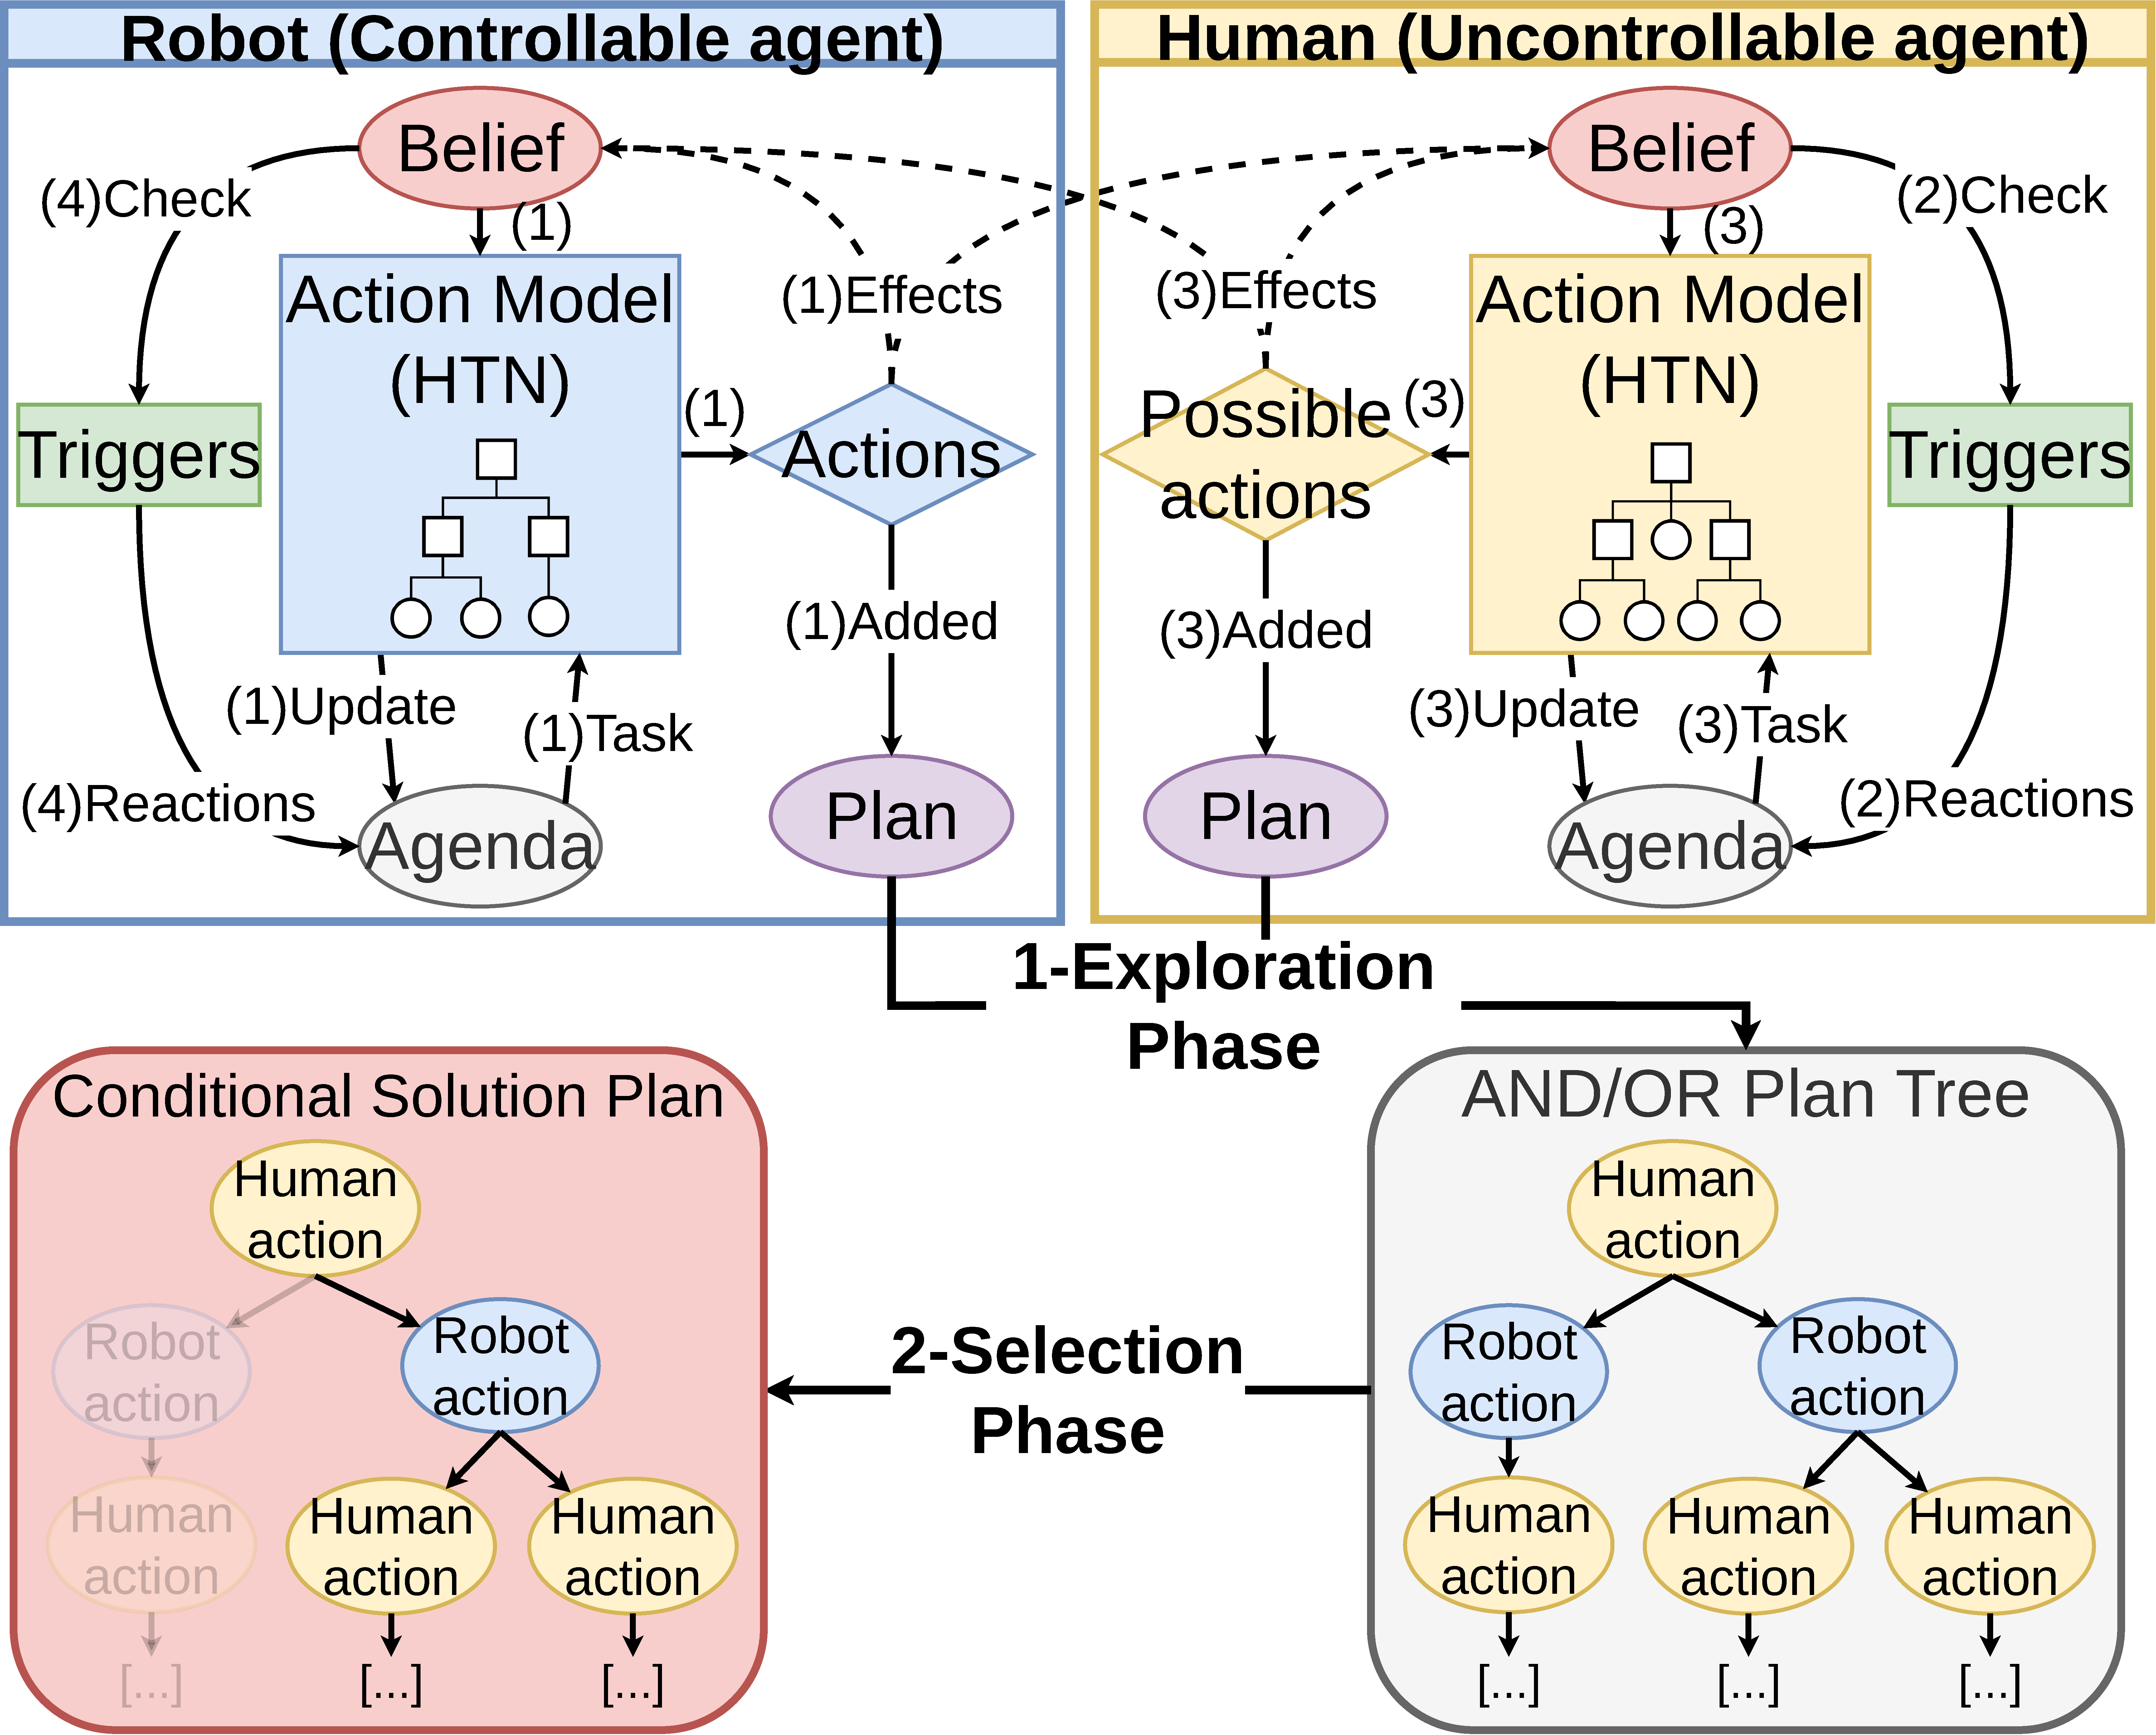
\includegraphics[width=\linewidth]{Chapter2/HATPEHDA_planning_process.pdf}
    \caption{The HTNs exploration consists in iterative loops of four steps : (1) Get possible robot actions from the robot HTN, add them to the plan and apply their specific effects on the H \& R beliefs, (2) Check Triggers and add the reactions in the corresponding agendas, (3) Get possible human actions based on their estimated beliefs, add them in the plan and apply their effects on the H \& R  beliefs, (4) Check Triggers again and add the reactions in the corresponding agendas. Here the robot is starting, but the human could with the following ordering: (3)>(4)>(1)>(2).}
    \label{fig:HATPEHDA_planning_process}
\end{figure}

The human \acrshort{htn} exploration differs from classical \acrshort{htn} planning as the goal is not to produce a complete plan but to list all the actions the human is likely to perform in a given agent state. 
We recursively decompose the first task of the human agenda $d^H$ with every applicable method until we reach an applicable operator. All the operators from all the applicable decompositions are returned to the robot HTN exploration and applied.

Two special cases are handled during the exploration. 
When an agent's agenda is empty, the exploration returns a default passive action \textit{IDLE}, which has no effect. It only indicates that the agent has nothing to do and will likely remain still. 
Besides, if no applicable action is found for an agent, the exploration returns a default passive action \textit{WAIT}. Similarly to \textit{IDLE}, it has no effect but represents the agent's impossibility to act in the current situation. 

Once both agendas are empty, the state is set as a success, the plan is added to the valid plans tree, and the search can continue until no decomposition is left for any task.


\section{Plan Evaluation and Selection}

In human-aware task planning, plan evaluation is a trade-off between efficiency and social criteria.
The robot should be efficient but also behave in an acceptable, legible, and accommodating manner.  


Cost evaluation is tricky because objective metrics are easy to use for efficiency. However, social criteria are more challenging to evaluate because they are hard to generalize. These social rules can be very context-dependent, making them hard to generalize and thus to take into account reliably.

Plan cost is a mix of all the following:

\begin{itemize}
    \item Length of the plan (number of actions or temporal duration if available).
    \item Sum of individual action cost: the cost of each action can be estimated to translate the effort required to perform it. It can reflect several aspects and constraints, such as pure physical strength required, duration of the action, or energy consumption.
    \item Undesired states: Common sense and social norms can be used to define several rules defining undesired states. This can cover various aspects such as hygiene or safety. For instance, despite being possible and maybe efficient, we would not like a robot holding a dirty dripping mop in one hand and the sandwich we asked for in the other hand. Another example is that we would not like a robot dropping a knife just on the edge of a table or counter because it may fall and be dangerous. 
    \item Undesired sequences of actions: For the same reasons, we can also define undesired sequences of actions. This can express preferences regarding the ordering of different subtasks, \textit{e.g.}, since we do not want the robot to hold our sandwich while cleaning the house, we would also not like the robot to clean first and then make a sandwich because the robot is likely to be dirty while making the sandwich.  
\end{itemize}

I implemented in HATP/EHDA a way to specify and take into account undesired state and action sequences. Detecting any of them in a possible plan would penalize the plan cost of the specified amount. Here, the undesired elements must be specified in the problem specification and are abstracted in the planner. However, as stated above, it is hard to generalize undesired states and action sequences and integrate them directly in the planner to avoid specifying them in the problem specification.

In HATP/EHDA, once the exhaustive exploration has been done, the result is a valid plan tree of alternating feasible robot and human actions along with their current beliefs leading to task completion. This second planning step aims to select robot actions, such as each human action in the plan has only one robot action as a child.
To do so, we define a cost function $cost: \sigma \times Op \mapsto \mathbb{R}^+$ representing the cost of an action in a specific state. The data structure is now similar to a two-player game tree. However, \textit{MinMax} approaches are unsuitable here, as we are not in an adversarial setup but more in a collaborative one. Indeed, trying to minimize the maximum possible cost assumes that humans will always do the actions that lead to the worst plan. This defensive behavior could lead to non-optimal plans. We thus propose to explore this tree differently.

Moreover, like in \acrshort{hatp}, we can define \textit{social costs} functions. These functions take a complete human and robot sequence of actions ($\pi^R$ and $\pi^H$) and return a cost ($\mathbb{R}^+$) which is added to the cost of the plan previously determined. By doing so, we can penalize non-acceptable sequence of robot actions (\textit{e.g.}serving a meal just after taking out the trash) or non-satisfactory human required contribution (\textit{e.g.}the robot requesting the human to perform small tasks multiple times instead of giving the big picture of the actual task to perform).

The approach we propose for plan selection is to minimize the average cost. It represents the human potentially selecting any course of action in their stream (while still respecting the action model defined in their HTN).
The algorithm is given the root action of the plan tree previously generated. It returns the cost of the conditional plan selected while selecting the robot actions in the plan tree to minimize the average plan cost.

\section{Qualitative Results}

Each scenario is commented on below with their corresponding selected plan shown in TABLE~\ref{tab:plans}.

The partial robot and human action models and their exploration are presented in Fig.~\ref{fig:plans}.

\begin{table}
\small
\begin{tabularx}{0.98\textwidth}{|X||X|}
    \hline
    \textbf{(a) \textit{R} and \textit{H1} build the stack together as a shared goal requested by \textit{H1}.}     & \textbf{(b) \textit{H1} requests to stack the cubes and \textit{R} acts alone.} \\
    \hline
    R-PickAndPlace(red, base)     & R-PickAndPlace(red, base) \\ 
    H1-PickAndPlace(red, base)     & R-moveTo(red) \\  
    R-PickAndPlace(green, bridge) & R-PickAndPlace(red, base) \\
    H1-PickAndPlace(blue, top)     & R-moveTo(init) \\
    R-PickAndPlace(yellow, top)   & R-PickAndPlace(green, bridge) \\
                                    & R-PickAndPlace(blue, top) \\
                                    & R-PickAndPlace(yellow, top) \\
    \hline \hline
    \textbf{(c) \textit{H1} requests R to build the stack, \textit{R} decides to punctually involve \textit{H2}.} & \textbf{(d) \textit{H1} requests R to build the stack, \textit{R} decides to invite H2 to a shared goal.} \\
    \hline
    R-PickAndPlace(red, base)     & R-PickAndPlace(red, base) \\
    H2-IDLE                        & H2-IDLE \\
    R-AskPunctualHelp(red)        & R-AskSharedGoal() \\
    H2-PickAndPlace(red, base)     & H2-PickAndPlace(red, base) \\
    R-PickAndPlace(green, bridge) & R-PickAndPlace(green, bridge) \\
    H2-IDLE                        & H2-PickAndPlace(blue, top) \\
    R-PickAndPlace(blue, top)     & R-PickAndPlace(yellow, top) \\
    H2-IDLE                        & \\
    R-PickAndPlace(yellow, top)   & \\
    \hline
\end{tabularx}
\caption{Execution trace of a selected plan for each scenario.}
\label{tab:plans}
\end{table}

\begin{sidewaysfigure}
    \centering 
    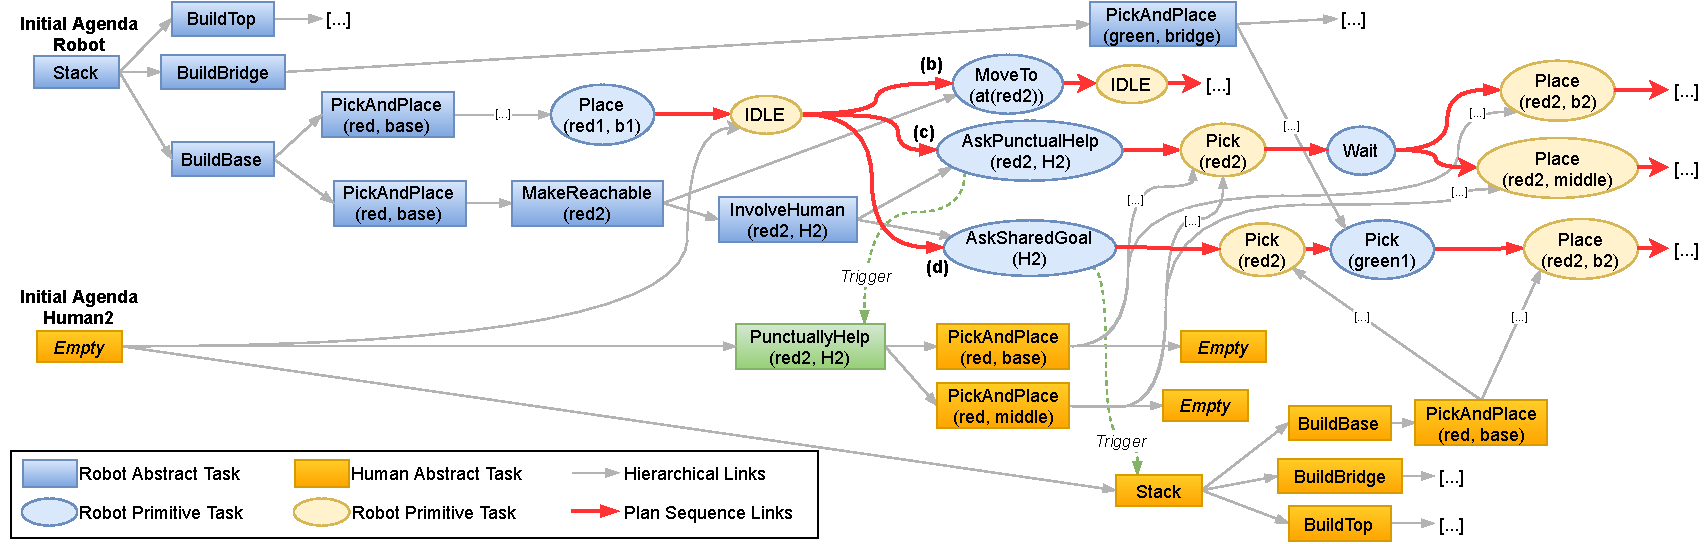
\includegraphics[width=1.0\textwidth]{Chapter2/plans.pdf}
    \caption{Illustration of the incremental exploration of various courses of actions corresponding to scenarios depicted in Fig.~\ref{fig:scenarios}(b), (c), and (d). Since \textit{H1} requests the robot to complete the task without establishing a shared goal, the robot agenda only contains the task to achieve, and the agenda of \textit{H2} starts empty.}
    \label{fig:plans}
\end{sidewaysfigure}

\paragraph{(a) \textit{H1} and R act together}
First, the human sets a shared goal by asking the robot to stack cubes with him. Since it is a shared goal, human and robot agendas are initialized with the ``Stack" task. Thus, the robot anticipates that the human will pick the unreachable second red cube by querying the human action model. Table~\ref {tab:plans}(a) shows the selected plan to collaboratively stack the cubes. 

\paragraph{(b) \textit{R} acts alone}
This time, the human asks the robot to stack the cubes but then leaves the scene, and the robot must act alone. Hence, the only applicable method to make the second red cube reachable is to move to the other side even though the movement action is expensive (we can imagine a table way longer than shown in the figure).

\paragraph{(c) \textit{R} asks punctual help}
The first human (\textit{H1}) requests the robot to complete the task, and another uninvolved human ($h2$) is present. The robot starts exploring its \acrshort{htn} and, thanks to the presence of the other human, a new method is applicable, allowing the robot to ask for help. It can ask for punctual help or a complete commitment of \textit{H2} to the task. Of course, asking for help for one cube is less costly than building the whole stack together. However, asking for help from someone not already involved in a common task is still expensive since they must put themselves in the task's context. 
Nevertheless, this punctual help is less costly for the robot than moving to the other side, so this solution is selected. Note that we model that after being asked to help punctually, the human can either stack the cube themself or make it reachable to the robot by placing it in the middle. Only the first branch is shown in table~\ref{tab:plans}(c), but the selected plan is in fact conditional with two branches as depicted in Fig.~\ref{fig:plans}.

\paragraph{(d) \textit{R} invites \textit{H2} to share a goal}
Same initial setup, but now two cubes are out of reach. Asking for punctual help is still less costly than moving around the table. 
However, each new request to \textit{H2} is assumed to be more and more costly, making repeated queries expensive.  
Therefore, due to the two unreachable cubes in this scenario, setting a shared goal becomes less costly for the robot than asking twice for punctual help.

\section{Conclusion}

What is offered by HATP/EHDA is very interesting. We rely and reason on the human model to plan the robot's actions while never compelling the human actions. The plan produced assumes turn-taking and no parallel execution of the actions. This is not a strict constraint as a post-analysis can reason on the causal links of the actions in the plan to extract a partially ordered plan to execute, making the execution more flexible. However, It is still a limitation addressed in Chapter~\ref{chap:4}.
% \ifdefined\included
\else
\setcounter{chapter}{2} %% Numéro du chapitre précédent ;)
\dominitoc
\faketableofcontents
\fi

\chapter{Models and Algorithms for human-aware task planning with integrated theory of mind}
\chaptermark{Models and Algorithms of Theory of Mind}
\label{chap:3}
\minitoc


%%% SECTION %%%%%%%%%%%%%%%%%%%%%%%%%%%%%%%%%%%%%%%%%%%%%%%%%%%%
\section{Introduction}

We would want the robot to be able to reason and maintain correctly the distinct human beliefs. Despite modeling distinct beliefs, HATP/EHDA doesn't maintain in a principled way, only in a scripted way (domain specific). Here we propose some models and algorithms to integrate some concept of Theory of Mind in the planning process of HATP/EHDA. This way, the robot can estimate more accurately the human's belief to predict their behavior. Moreover, we propose solutions for the robot when to tackle estimated false human beliefs that may impact the task resolution.

Explaining false belief task (Sally and Anne)
\begin{figure}
    \centering
    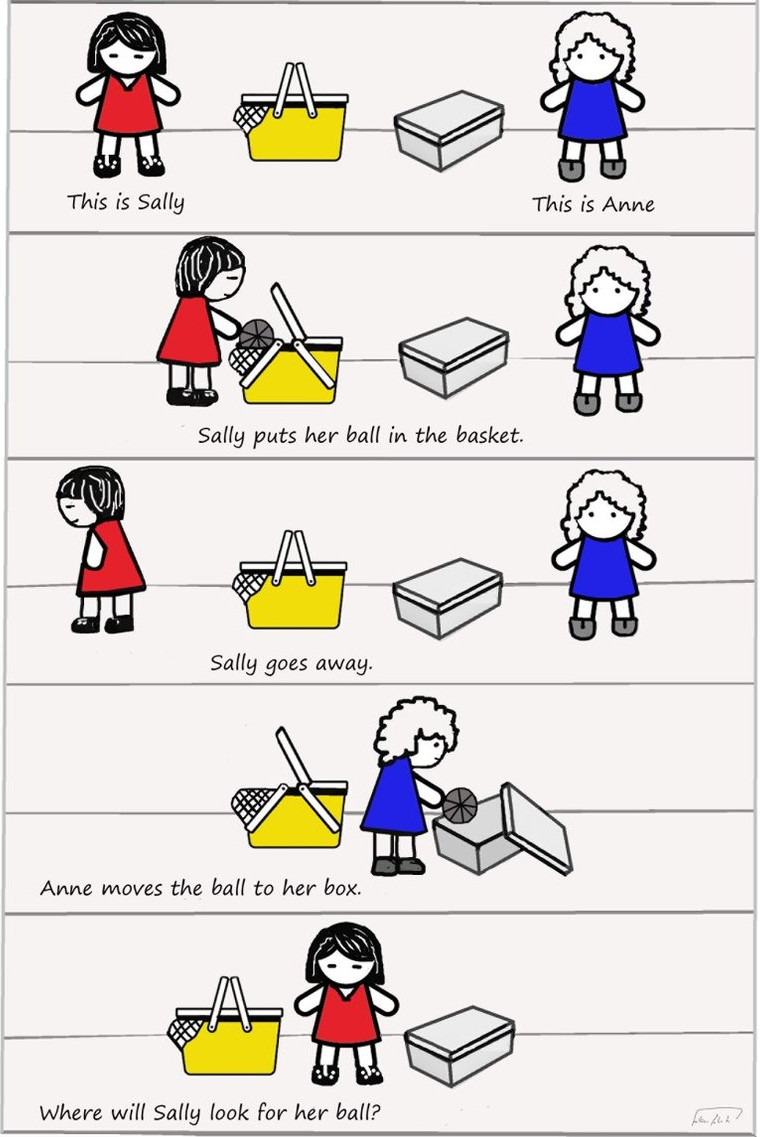
\includegraphics[width=0.5\linewidth]{images/Chapter3/The-Sally-Anne-Task.jpeg}
    \caption{Sally and Anne Task}
    \label{fig:sally_and_anne_ask}
\end{figure}



%%% SECTION %%%%%%%%%%%%%%%%%%%%%%%%%%%%%%%%%%%%%%%%%%%%%%%%%%%%
\section{Related works}

    This chapter's contribution is related to several topics not mentioned yet. Hence, to better capture the contribution, this section introduces the new topics and relevant related works.  

    %%% SUB-SECTION %%%%%%%%%%%%%%%%%%%%%%%%%%%%%%%%%%%%%%%%%%%%
    \subsection{Epistemic planning}
    Epistemic planning plays a crucial role in human-robot collaboration. It allows robots to reason about their own knowledge and beliefs, as well as the knowledge and beliefs of other agents \cite{bramblett_epistemic_2023}. This is important for coordination and collaboration among multiple agents, as success can only be expected if agents can reason about each other's knowledge, uncertainty, and capabilities \cite{bramblett_epistemic_prediction_2023}. Epistemic planning is used in various application areas, including mobile service robots, explaining planning, game playing, human-robot interaction, and social robotics \cite{hu_planning_2023}. It enables robots to make plans to achieve the required knowledge and to reason about the knowledge and capabilities of other agents, ensuring effective collaboration and coordination in human-robot interactions \cite{belle_epistemic_2023}.


    Def. Thomas Bolander is one of the main contributor to this field. Proposed the DEL approach. \cite{bolander_gentle_2017} and extended it.

    ``Automated planning is a branch of artificial intelligence concerned with computing plans (sequences of actions) leading to some desired goal. A human or robot could e.g. have the goal of picking up a parcel at the post office, and then the problem becomes to find a successful sequence of actions achieving this. Epistemic planning is the enrichment of planning with epistemic notions, that is, knowledge and beliefs. The human or robot might have to reason about epistemic aspects such as: Do I know at which post office the parcel is? If not, who would be relevant to ask? Maybe the parcel is a birthday present for my daughter, and I want to ensure that she doesn't get to know, and have to plan my actions accordingly (make sure she doesn't see me with the parcel). The epistemic notions are usually formalized using an epistemic logic. Epistemic planning can naturally be seen as the combination of automated planning with epistemic logic, relying on ideas, concepts and solutions from both areas.''

    Muise et al. worked on multi-agent epistemic planning using a classical planning approach. Since involving nested beliefs is computationally demanding, their work proposes to convert and encode such problems into classical planning problems. Hence, state-of-the-art classical planning technics can be used to tackle nested beliefs of multiple agents problems. 

    \subsection{Theory of Mind in HRC}
    Epistemic planning helps to plan the correct sequence of actions to perform to reach a desired knowledge, including a desired world state. However, estimating the current knowledge and beliefs of the different agents is challenging. To do so, we have to consider Theory of Mind concepts, especially perspective shift and the notion of co-presence. Some epistemic planning works already integrate of ToM notions, but the subject is worth being discussed a bit more in details. Indeed, in the HRI field, ToM is used in various domains like navigation, dialogue and like here in task planning. 

    Theory of mind (ToM) plays a crucial role in task planning for human-robot collaboration. 
    ToM refers to the ability to attribute mental states to oneself and others, such as beliefs, desires, and intentions. 
    
    (v1) Robots endowed with ToM abilities can anticipate and understand the mental states of their human partners, allowing for more effective interaction and decision-making. By inferring their partner's trust and strategy, robots can adjust their own decision models and policies to optimize team performance [1]. Mimicking ToM in robots influences human decision-making behavior and trust, making it more appropriate and conducive to collaboration [2]. Robots implementing ToM are perceived as more socially intelligent and helpful, enhancing the quality of human-robot interactions [3]. Computational theory of mind, based on abstractions of beliefs into higher-level concepts, enables agents to reason and collaborate with humans efficiently, improving decision-making outcomes [4]. However, the field lacks a unified construct and consistent benchmarking, hindering progress in endowing robots with ToM capabilities [5].

    (v2) Robots endowed with ToM abilities are more effective in proactive robotic assistance and are perceived as more socially intelligent by humans \cite{shvo_proactive_2022}. ToM enables robots to infer human desires, beliefs, and intentions, allowing for natural interaction between robots and humans \cite{yu_robot_2023}. Robots with ToM can anticipate human strategies and incorporate them into their decision models, leading to better team performance \cite{romeo_exploring_2022}. The presence of ToM in robots influences human decision-making behavior and trust, making it more appropriate for human-robot collaboration \cite{schlobach_abstracting_2022}. Computational theory of mind, based on abstractions of beliefs into higher-level concepts, facilitates collaboration on decisions and improves the quality of human decisions \cite{gurney_robots_2022}. However, the lack of a unified construct and consistent benchmarking hinders progress in endowing robots with ToM capabilities.

    \textbf{TODO: Merge two versions, but references of v1 are not accessible anymore...}

    
    \subsection{Communication in HRC}

    Communication plays a crucial role in human-robot collaboration. It enables effective interaction between humans and robots, promoting inclusivity and reducing obstacles in human-robot interaction. Communication allows robots to share information about their actions and intentions, enhancing transparency and explainability \cite{mcmillan_human-robot_2023}. It helps in establishing trust and understanding between humans and robots, leading to improved teamwork and performance \cite{verhagen_influence_2022}. Non-verbal gestures and behavior of robots during collaboration can impact the perception of the robot and influence the willingness of humans to cooperate \cite{arntz_collaborating_2022}. Communication also allows robots to assess their own skills and limitations, propose alternatives, and adapt the execution of tasks to the capabilities of the collaborators \cite{ferrari_bidirectional_2022}. Overall, effective communication facilitates mutual knowledge, enables the exchange of information, and allows humans and robots to work together efficiently and successfully.


%%% SECTION %%%%%%%%%%%%%%%%%%%%%%%%%%%%%%%%%%%%%%%%%%%%%%%%%%%%
\section{Maintaining the human beliefs}

    %%% SUB-SECTION %%%%%%%%%%%%%%%%%%%%%%%%%%%%%%%%%%%%%%%%%%%%
    \subsection{Enhanced problem specification}

\textbf{TODO: switch from 'we' to 'I'?}

\begin{figure}[t!]
    \centering
    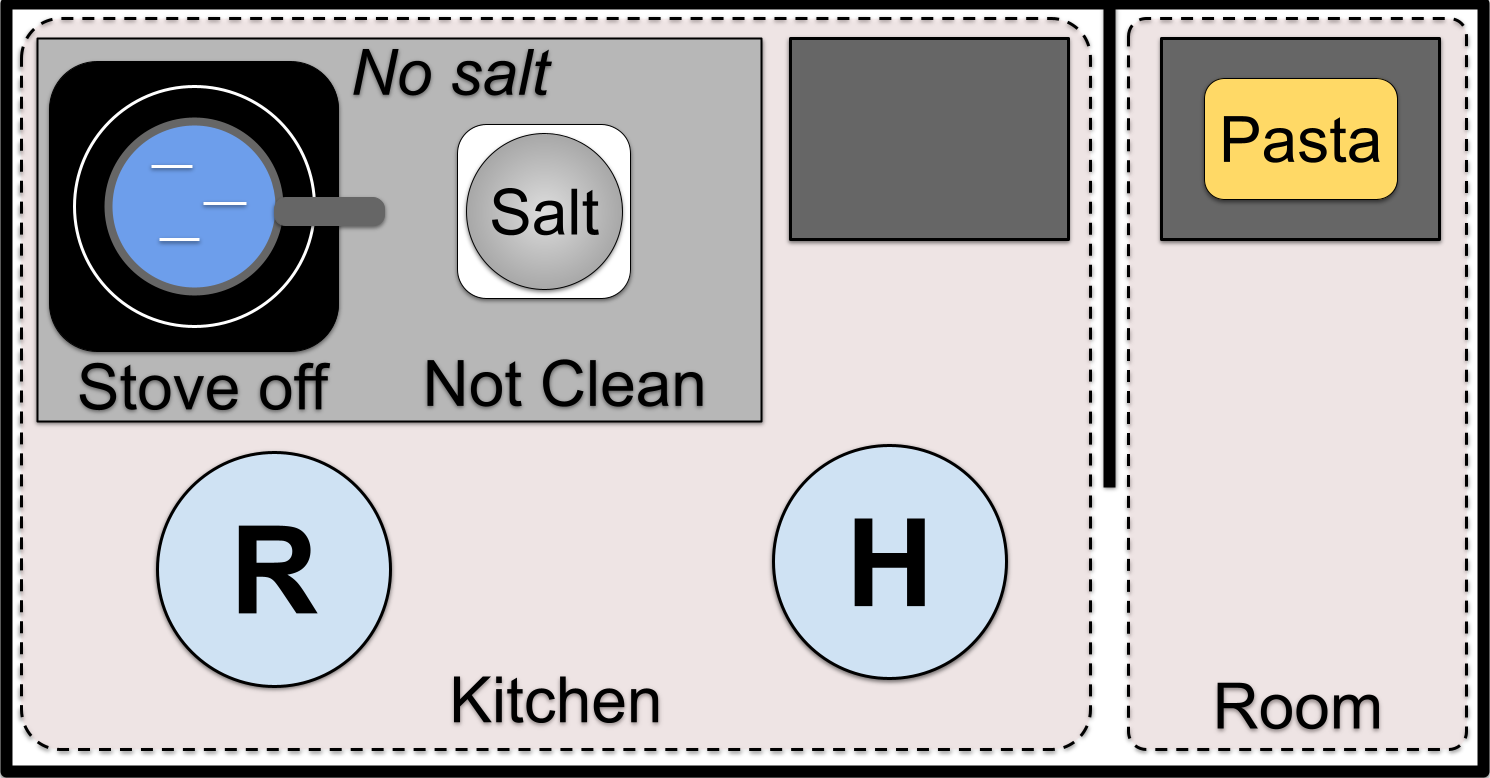
\includegraphics[width=0.70\linewidth]{images/Chapter3/cooking_task_draw.png}
    \caption{
    Let us consider cooking pasta as a human-robot shared task. 
    The robot has to turn on the stove (\textit{stoveOn}) and clean the counter (\textit{counterClean}), but the latter is not a part of the shared task. The human takes care of fetching the pasta while both agents can add salt into the water (\textit{saltIn}). Before pouring the pasta into the pot the human must know the facts, \textit{stoveOn} and \textit{saltIn}. 
    Unlike \textit{stoveOn}, the facts \textit{saltIn} and \textit{counterClean} are not directly observable. 
    Hence, by acting while the human is away to fetch the pasta, the robot may induce false beliefs which may be detrimental to the shared task (e.g., human adding salt again).
    }
    \label{fig:new_scene}
\end{figure}

We start from the HATP/EHDA probleme specification which is the following.

We consider a \textit{classical planning domain} (\textit{state-transition system}) $\Sigma = (S,A,\gamma)$, s.t., $S$ is a finite set of states in which the system may be, $A$ is a finite set of actions that the actors may perform, $\gamma : S \times A \rightarrow S$ is a state-transition function. Each state $s \in S$ is a description of the properties of various objects in the planner's environment~\cite{naubooks0014222}. 

To represent the objects and their properties, we will use two sets $B$ and $X$: $B$ is a set of names for all the objects, plus any mathematical constants representing properties of those objects. $X$ is a set of syntactic terms called state variables, s.t. the value of each $x \in X$ depends solely on the state $s$.

A \textit{state-variable} over $B$ is a syntactic term $x = sv(b_1, ..., b_k)$, where $sv$ is a symbol called the state variable's name, and each $b_i$ is a member of $B$ and a parameter of $x$. Each state variable $x$ has a range, $\textit{Range}(x) \subseteq B$, which is the set of all possible values for $x$.

Here is the description of the sets $B$ and $X$ for the collaborative cooking example:
{\small
\begin{align*}
&B           = Entities \cup Places \cup Booleans \cup \{\textsf{nil}\} \\
&\quad Entities    = Agents \cup Objects\\
&\quad Agents      = \{ \textsf{R}, \textsf{H} \} ~~ \backslash\backslash~\textsf{R}:robot,~\textsf{H}:human\\
&\quad Objects     = \{ \textsf{salt}, \textsf{pasta}, \textsf{counter} \}\\
&\quad Places      = \{ \textsf{kitchen}, \textsf{room} \}\\
&\quad Booleans    = \{ \textsf{true},\textsf{false} \}\\
&\\
&X = \{ at(e), saltIn, stoveOn, counterClean ~ | ~ e \in Entities \}\\
&\quad \textit{Range}(saltIn ~|~ stoveOn ~|~ counterClean)=Booleans\\
&\quad \textit{Range}(at(\textsf{R} ~|~ \textsf{H} ~|~ \textsf{pasta})) = Places\\
&\quad \textit{Range}(at(\textsf{salt} ~|~ \textsf{counter})) = \{ \textsf{kitchen} \}
\end{align*}
}

A \textit{variable value assignment} function over $X$ is a function $val$ that maps each $x_i \in X$ into a value $z_i \in$ $\textit{Range}(x_i)$. With $X = \{ x_1, ..., x_n \}$, we will often write this function as a set of assertions: $val = \{ x_1=z_1, \ldots, x_n=z_n \}$. 

Our first contribution starts from here where we augmented the specification by associating each state variable to a location and to an observability type.

A \textit{variable observability assignment} function over $X$ is a function $obs$ that maps each $x_i \in X$ into an observability type $t_i \in \{ \texttt{OBS},  \texttt{INF} \}$: $obs = \{ (x_1,t_1), \ldots , (x_n,t_n) \}$. Respectively, when $obs(x_i) = \texttt{OBS} | \texttt{INF}$ then $x_i$ is said to be \textit{observable} $|$ \textit{inferable} in the state $s_i$.

A \textit{variable location assignment} function over $X$ is a function $loc$ that maps each $x_i \in X$ into a $l_i \in Places \cup \{ \texttt{nil} \}$: $loc = \{ (x_1,l_1), ..., (x_n,l_n) \}$. 
$Places \subseteq B$ captures a group of constant symbols such that each member is a predefined area in the environment. 
Agents are always either ``situated'' in a place or moving between two places. 
We consider $x_i$ to be located in every $place \in Places$ if $loc(x_i)=\texttt{nil}$. 
More details about how the environment should be divided into places will be given shortly.

A \textit{state} $s_i \in S$ is a 6-tuple composed of 4 functions over $X$ and 2 task networks (agendas)  s.t. $s_i = (val_i, val^H_i, obs_i, loc_i, tn^R_i, tn^H_i)$. 
The state of the world from the perspective of the robot is captured by the variable value assignment function $val_i$, sometimes noted as $val^R_i$. 
Similarly, $val^H_i$ represents the estimation of $val_i$ in the perspective of the human, also referred to as the estimated human beliefs. 
Hence, $\forall s_i \in S$, each $x_j \in X$ is  mapped to two \textit{values} (robot perspective and estimation of human's beliefs), an \textit{observability type}, and a \textit{place}. We say that a state $s_i \in S$ contains \textit{false beliefs}, or \textit{belief divergences}, if $\exists x_j \in X, val^H_i(x_j) \neq val^R_i(x_j)$. 

For our example, the initial state $s_0$ would be as follow: 

\newcommand{\smallvspace}{\vspace{-0.8cm}}
\newcommand{\bigvspace}{\vspace{-1.3cm}}

{\small
\noindent
\begin{multline*}
s_0 = \{val_0, ~val^H_0, ~obs_0, ~loc_0, ~tn^R_0, ~tn^H_0\} \\ \quad
\end{multline*}
\bigvspace
\begin{multline*}
\quad val_0 = val^H_0 = \{at(\textsf{R}) = \textsf{kitchen}, at(\textsf{H}) = \textsf{kitchen},\\ 
at(\textsf{pasta}) = \textsf{room}, saltIn = \textsf{false}, stoveOn=\textsf{false} \}
\end{multline*}
\smallvspace
\begin{multline*}
\quad obs_0=\{ (at(e),\texttt{OBS}),
(saltIn,\texttt{INF}),
(stoveOn,\texttt{OBS})\\
(counterClean,\texttt{INF}),
~|~ e \in Entities \}
\end{multline*}
\smallvspace
\begin{multline*}
\quad loc_0=\{ (at(e),val_0(e)),
(counterClean,\textsf{kitchen}),\\
(saltIn,\textsf{kitchen}),
(stoveOn,\textsf{kitchen}),
~|~ e \in Entities \}
\end{multline*}
\smallvspace
\begin{multline*}
\quad tn^R_0 = \{ CookPasta, CleanCounter \} \\ \quad
\end{multline*}
\bigvspace
\begin{multline*}
\quad tn^H_0 = \{ CookPasta \} \\ \quad
\end{multline*}
\smallvspace
}

An action is a tuple $\alpha = (\textit{head}(\alpha), \textit{pre}(\alpha), \textit{eff}(\alpha))$ where $\textit{head}(\alpha)$ is a syntactic expression of the form $\textit{act}(z_1, ..., z_k)$ where $act$ is a symbol called the \textit{action name} and $z_1,...,z_k$ are variables called parameters. $\textit{pre}(\alpha) = \{ p_1, ..., p_m \}$ is a set of preconditions, each of which is a literal. And $\textit{eff}(\alpha) = \{ e_1, ..., e_n \}$ is a set of effects, each of which is an expression of the form: $sv(t_1, ..., t_j) \leftarrow t_0$ with $t_0$ being either the value to assign to the state variable $sv(t_1, ..., t_j)$ or a new location/place for the state variable. We note $\textit{agt}(\alpha)$ the agent performing the action $\alpha$.

To estimate the next possible actions that an agent $\varphi \in Agents$ is likely to perform in a state $s_i \in S$, we proceed in the same way as in~\cite{buisan:hal-03684211}. We refine the agent's agenda $tn_{\varphi}$ based on its belief $val^\varphi_i$ and obtain a \textit{refinement} as follows $\textit{ref}(tn^\varphi_i, val^\varphi_i)= \{ (a_1,tn_1),...,(a_j,tn_j) \}$. 
A \textit{refinement} contains a tuple for each estimated possible action $a_j$ and the associated new agenda $tn_j$ after being refined. 

In our cooking example, we obtain the following refinement if the starting agent is the human:\\
{\small
$\textit{ref}(tn^H_0, val^H_0) = \{ (add\_salt(),tn_1), (move\_to(\textsf{kitchen}),tn_2) \}$
}


    %%% SUB-SECTION %%%%%%%%%%%%%%%%%%%%%%%%%%%%%%%%%%%%%%%%%%%%
    \subsection{State Transitions and Beliefs Updates}
Learn from observation of either: action execution or observable state.

Assumption 1 : We do not consider uncertainties. Thus, agents are either wrong or right about the state of the world but never uncertain. This would be an interesting future work. 

Assumption 2 : We do not consider cases where the robot's beliefs can diverge. Since the planner is part of the robot, the actual ground truth is unknown. We can only assume that the estimation of the state of the world by the robot is correct and reason on it.

Assumption 3 : Coming from the two previous assumptions, we assume that the human only makes deterministic moves when not being observed. Hence, regardless of being co-present, the robot's beliefs are always updated with the action's effects.


Thus, $\forall x \in X$, we always have,

\begin{equation}
    val_{i+1}(x) = \left\{ 
    \begin{array}{ll}
        w, & \mbox{if} ~ x \leftarrow w \in \textit{eff}(a)   \\ 
        val_i(x), & \mbox{otherwise}
    \end{array}\right.
\end{equation}

The place associated with a state variable can be modified by the action's effect but, here, we assume that the observability type of each fact is constant during the task. So, $\forall x \in X$,

\begin{align}
    &obs_{i+1}(x) = obs_i(x)\\
    &loc_{i+1}(x) = \left\{ 
    \begin{array}{ll}
        l, & \mbox{if} ~ x \leftarrow l \in \textit{eff}(a)\\
        loc_i(x), & \mbox{otherwise}
    \end{array}\right.
\end{align}

The new agenda of each agent ($tn^R_{i+1}, tn^H_{i+1}$) are created by the HTN refinement algorithm, and thus, they are directly retrieved from the obtained refinement. 
This refinement decomposes abstract tasks in the task network until the first task is a primitive action. To do so, every applicable method is applied leading to a set of possible actions (and refined task networks).

The new estimated human belief $val^H_{i+1}$ is the two-step result of our Situation Assessment processes that models the human's real-time sensing and reasoning capabilities about their surroundings.

First, let us define the notions of \textit{co-presence} and \textit{co-location} which will be key to maintaining the evolution of agents' beliefs as planning progresses.

\begin{definition} \label{def:co-pre-loc}
    \textbf{(Co-presence \& Co-location.)} In a state $s_i \in S$, two agents, $\varphi_1$ and $\varphi_2$, are considered to be \textit{co-present} if $val_i(at(\varphi_1)) = val_i(at(\varphi_2))$. This relation is noted $\varphi_1 \curlywedge_i \varphi_2$ in the rest of the paper. Similarly, we say that an agent $\varphi_1$ is \textit{co-located} with a state variable $x \in X$ if $val_i(at(\varphi_1)) = loc_i(x)$, noted $\varphi_1 \curlywedge_i x$.
\end{definition}

Now we can define two SA processes that will maintain the estimated human beliefs.

\begin{definition} \label{def:new_inf}
    \textbf{(Inference Process.)} An agent observes the execution of an action by being either co-present with the acting agent, 
    or by being the acting agent. If so, the agent infers the new values of every state variable present in the action's effects.
\end{definition}

Based on the above definition, the human's beliefs are updated as follows when action $a$ is executed in state $s_i$, 

\begin{equation}
val'^H_{i+1}(x) = \left\{ 
\begin{array}{ll}
    w, & \mbox{if} ~ x \leftarrow w \in \textit{eff}(a) ~ \mbox{and}  \\ 
    & (H = \textit{agt}(a) ~\mbox{or}~ H \curlywedge_i \textit{agt}(a)\\
    & ~\mbox{or}~ H \curlywedge_{i+1} \textit{agt}(a))\\
    val^H_i(x), & \mbox{otherwise}
\end{array}\right.
\end{equation}

To change its \textit{place} in the environment, agents would use a dedicated \textit{``move''} action, such that its effect only updates the agent's location. 

\begin{definition} 
\label{def:new_obs}
    \textbf{(Observation Process.)} An agent observes its surroundings and assesses the exact value of each state variable located in the same place (i.e., each state variable the agent is co-located with).
\end{definition}

After applying the effects of an action to obtain $val_{i+1}$ and the human beliefs $val'^H_{i+1}$ (using the inference process), the observation process is executed. It updates again the estimated human beliefs with the facts currently observable by the human and provides fully updated human beliefs to store in the state $s_{i+1}$, $\forall x \in X$:

\begin{equation}
val^H_{i+1}(x) = \left\{ 
\begin{array}{ll}
val_{i+1}(x), & \mbox{if}~ H \curlywedge_{i+1} x ~\mbox{and}~ \\
    & obs_{i+1}(x) = \texttt{OBS}\\
val'^H_{i+1}(x), & \mbox{otherwise}
\end{array}\right.
\end{equation}

Note that before starting the planning process, the observation process is executed once on the initial state $s_0$. This allows us to potentially correct the estimated human beliefs with the facts the human should initially be able to observe. 

The definition of the set $Places$, i.e. how the environment is divided into different \textit{places}, is guided by the shape of our state transition function. Hence, a $place \in Places$ is an area in the environment such that, when situated in it, agents are aware of each other's activity and they can assess every observable fact located in it. 

Note that unlike in DEL~\cite{KR2021-12}, our knowledge representation is simple and prevents us from expressing agents being \textit{uncertain} about a fact. 
In line with the classical closed-world assumptions, agents either know the truth or have a false belief w.r.t. the ground truth. 
We consider a straightforward scenario in which the human is \textit{``unaware''} of non-observed changes in the environment. 
This results in estimated false human beliefs, helping to detect whether a non-observed robot action can disrupt a seamless collaboration. 

%%% SECTION %%%%%%%%%%%%%%%%%%%%%%%%%%%%%%%%%%%%%%%%%%%%%%%%%%%%
\section{Relevant False human beliefs}

In this section, we explain our procedure to detect \textit{when} a false human belief should be corrected and \textit{how}.


    %%% SUB-SECTION %%%%%%%%%%%%%%%%%%%%%%%%%%%%%%%%%%%%%%%%%%%%
    \subsection{Detection}

The human and the robot carry individual distinct beliefs, while the two can be aligned, or diverging when the human has a false belief. To produce a legal solution plan the robot is fine with such false human beliefs unless they are qualified as \textit{relevant} (Definition~\ref{def:relevant_false_belief}). In such cases, the relevant false belief needs to be tackled.

\begin{definition} \label{def:relevant_false_belief}

A \textbf{relevant false belief} is a false belief that influences the next action(s) the human is likely to perform, either in terms of number, name, parameters, or effects. This can be written as follows:
A state $s_i$ contains a relevant false belief if either (\ref{eq:rel_div_cond_1}) or (\ref{eq:rel_div_cond_2}) is true:

\begin{equation} \label{eq:rel_div_cond_1}
ref(tn^H_i, val^H_i) \neq ref(tn^H_i, val^R_i)
\end{equation}
\begin{equation} \label{eq:rel_div_cond_2}
\{ \gamma(s_i,a) ~|~ \forall a \in ref( tn^H_i, val^H_i ) \} \neq \{ \gamma(s_i,a) ~|~ \forall a \in ref( tn^H_i, val^R_i ) \}
\end{equation}
\end{definition}

We consider that as soon as a false belief has an effect on human actions it should be tackled. An interesting future work could  be to check in a principled way the overall positive and detrimental impacts of this false belief on collaboration. But it is out of the scope of this work.

    %%% SUB-SECTION %%%%%%%%%%%%%%%%%%%%%%%%%%%%%%%%%%%%%%%%%%%%
    \subsection{Resolution with minimal communication}

A state containing a false human belief marked as \textit{relevant} must be handled. 
The first way to do it is by planning communication actions such that the robot communicates only the required facts to the human. This allows to correct false human beliefs that are relevant, but false beliefs that are \textit{``non-relevant''} will remain. 

\subsubsection{Modeling Communication Actions} 
We propose a generic communication action schema ($ca$) in this context. 
An agent $\varphi_i$ can \textit{communicate} an assertion $x=z$ (with $x \in X$ and $z \in$ Range($x$)) \textit{via} the action $ca_{\varphi_i, \varphi_j}(x,z)$ if $val^{\varphi_i}(x) = z$ and $val^{\varphi_j}(x) \neq z$.
The effect of $ca_{\varphi_i, \varphi_j}(x,z)$ corresponds to $val^{\varphi_j}(x) \leftarrow z$. Such actions are considered equally costly and instantaneous.

\subsubsection{Communicate Only the Required Facts}
Definition~\ref{def:relevant_false_belief} indicates if there is at least one diverging state variable in the human beliefs causing adverse effects, but without identifying which one(s).
Hence, we explain a subroutine below with the three steps, describing how we first identify the pertinent state variables to align, and then how the corresponding communication actions are created and inserted into the robot's plan.

\begin{enumerate}
    \item 
    \textit{Store} each state variable whose value differs in the human beliefs from the robot beliefs: $X_{diff} = \{ x ~|~ x\in X, val^H_i(x) \neq val^R_i(x) \}$.

    \item
    \textit{Build}, for each stored state variable $x \in X_{diff}$, a communication action $ca_{R, H}(x,val^R_i(x))$, all stored in a set $\mathit{CA}_{diff}$.

    \item 
    \textit{(Breadth-First Search.)} 
    The \textit{source} is $s_i$. Applying each $ca \in \mathit{CA}_{diff}$ generates a new state by aligning \textit{exactly} one state variable in the human beliefs s.t. $s'_i = \gamma(s_i, ca )$. 
    The search continues until the first state $s'_i$ selected to expand doesn't contain a relevant false belief. The communication actions used from the root until this selected state are \textit{retrieved} in a set $\mathit{CA}$.
\end{enumerate}

Once the above subroutine finishes, the retrieved communication actions in the set $\mathit{CA} = \{ ca_{R, H}(x_1,val^R_i(x_1)),..., ca_{R, H}(x_j,val^R_i(x_j)) \}$ must be inserted in the plan for belief alignment. Thus, Definition~\ref{def:joint-sol-plan} is redefined to be sound w.r.t. our approach. An edge can now either be a human action $o^h$ or a robot action $o^r$ with a set of communication action $CA$.
At each step, humans perform \textit{Observation}, while the robot executes each communication action $ca \in \mathit{CA}$, making the human's belief to \textit{update instantaneously}.

The set $\mathit{CA}$ is inserted before the diverging human actions and after the closest state where agents are co-present. 
But it could be interesting to reason with a better plan evaluation system to find the best place to insert this set.

    %%% SUB-SECTION %%%%%%%%%%%%%%%%%%%%%%%%%%%%%%%%%%%%%%%%%%%%
    \subsection{Resolution by delaying non-observed robot action}

So far we relied on communication, but depending on the environment (e.g. noisy), communication can be cognitively demanding. 
Thus, when the relevant false belief is due to a non-observed robot action, we propose to also consider implicit communication by postponing the pertinent robot action until the human is estimated to be observing its execution. 
This prevents false beliefs from even occurring.

First, a branch using communication is explored and the state variables concerned by the relevant false beliefs are retrieved (through all $ca \in CA$).
Then we check if the divergence is produced by a non-observed action. For now, it is done by checking if the relevant divergence concerns only one inferable state variable and if it was not present in the initial state.   
After, we identify which action creates the divergence by sequential regressing the current branch/trace. Hence, we can identify when the relevant divergence appears and which action should be delayed.
Once identified, we create another branch in the plan just before the identified action. In this new branch, {\sc delay} actions are inserted in the robot's plan until the human is co-present. When the human is co-present again, the identified action is inserted and observed by the human. Then the nominal planning process is resumed.  

%%% SECTION %%%%%%%%%%%%%%%%%%%%%%%%%%%%%%%%%%%%%%%%%%%%%%%%%%%%
\section{Result}

Referring to the related work section, we are not aware of an implemented planning system that can be used as a baseline. Hence, we use the HATP/EHDA solver to help present our approach's results on three \textit{novel} planning domains.

\subsubsection{Cooking Pasta Domain}
The running example corresponds to a specific problem in this domain. In fact, agents and pasta can initially either be in the kitchen or in the adjacent room, the stove might be on or off and there might be salt or not in the water.  
In the results, we will focus on the following three state variables from $X$. Both $stoveOn$ ($\texttt{OBS}$) and $saltIn$ ($\texttt{INF}$) are relevant to the human, unlike $Clean$ ($\texttt{INF}$) which only concerns the robot. 

\subsubsection{Preparing Box Domain}
A box with a sticker on it and filled with a fixed number of balls is considered prepared and needs to be sent. Both agents can \textit{fill} the box with balls from a bucket, while only the robot can \textit{paste} a sticker and only the human can \textit{send} the box. The bucket can run out of balls, so when one ball is left, the human \textit{moves} to another room to \textit{grab} more balls and \textit{refill} it. 
The number of balls in the box is \textit{inferable}, while all other variables are {\em observable}. 
In the following, three boxes have been considered.

\subsubsection{Car Maintenance Domain}
The washer fluid ($\texttt{OBS}$) and engine oil ($\texttt{INF}$) levels have to be \textit{full} before \textit{storing} the oil gallon in the cabinet ($\texttt{INF}$). 
Only the robot can \textit{refill} both the tanks and store the gallon while situated at \textit{Front} of the car. 
\textit{Front-left} and \textit{Front-right} headlights have to be \textit{checked} and a light-bulb has to be \textit{replaced} at \textit{Rear}. 
Only the human can check and replace lights, and they can start with either of these two tasks.
Both agents start at \textit{Front}.
The car's hood needs to be \textit{closed} by the human at last.

\subsection{Qualitative Analysis}

\begin{figure}[t!]
    \centering
    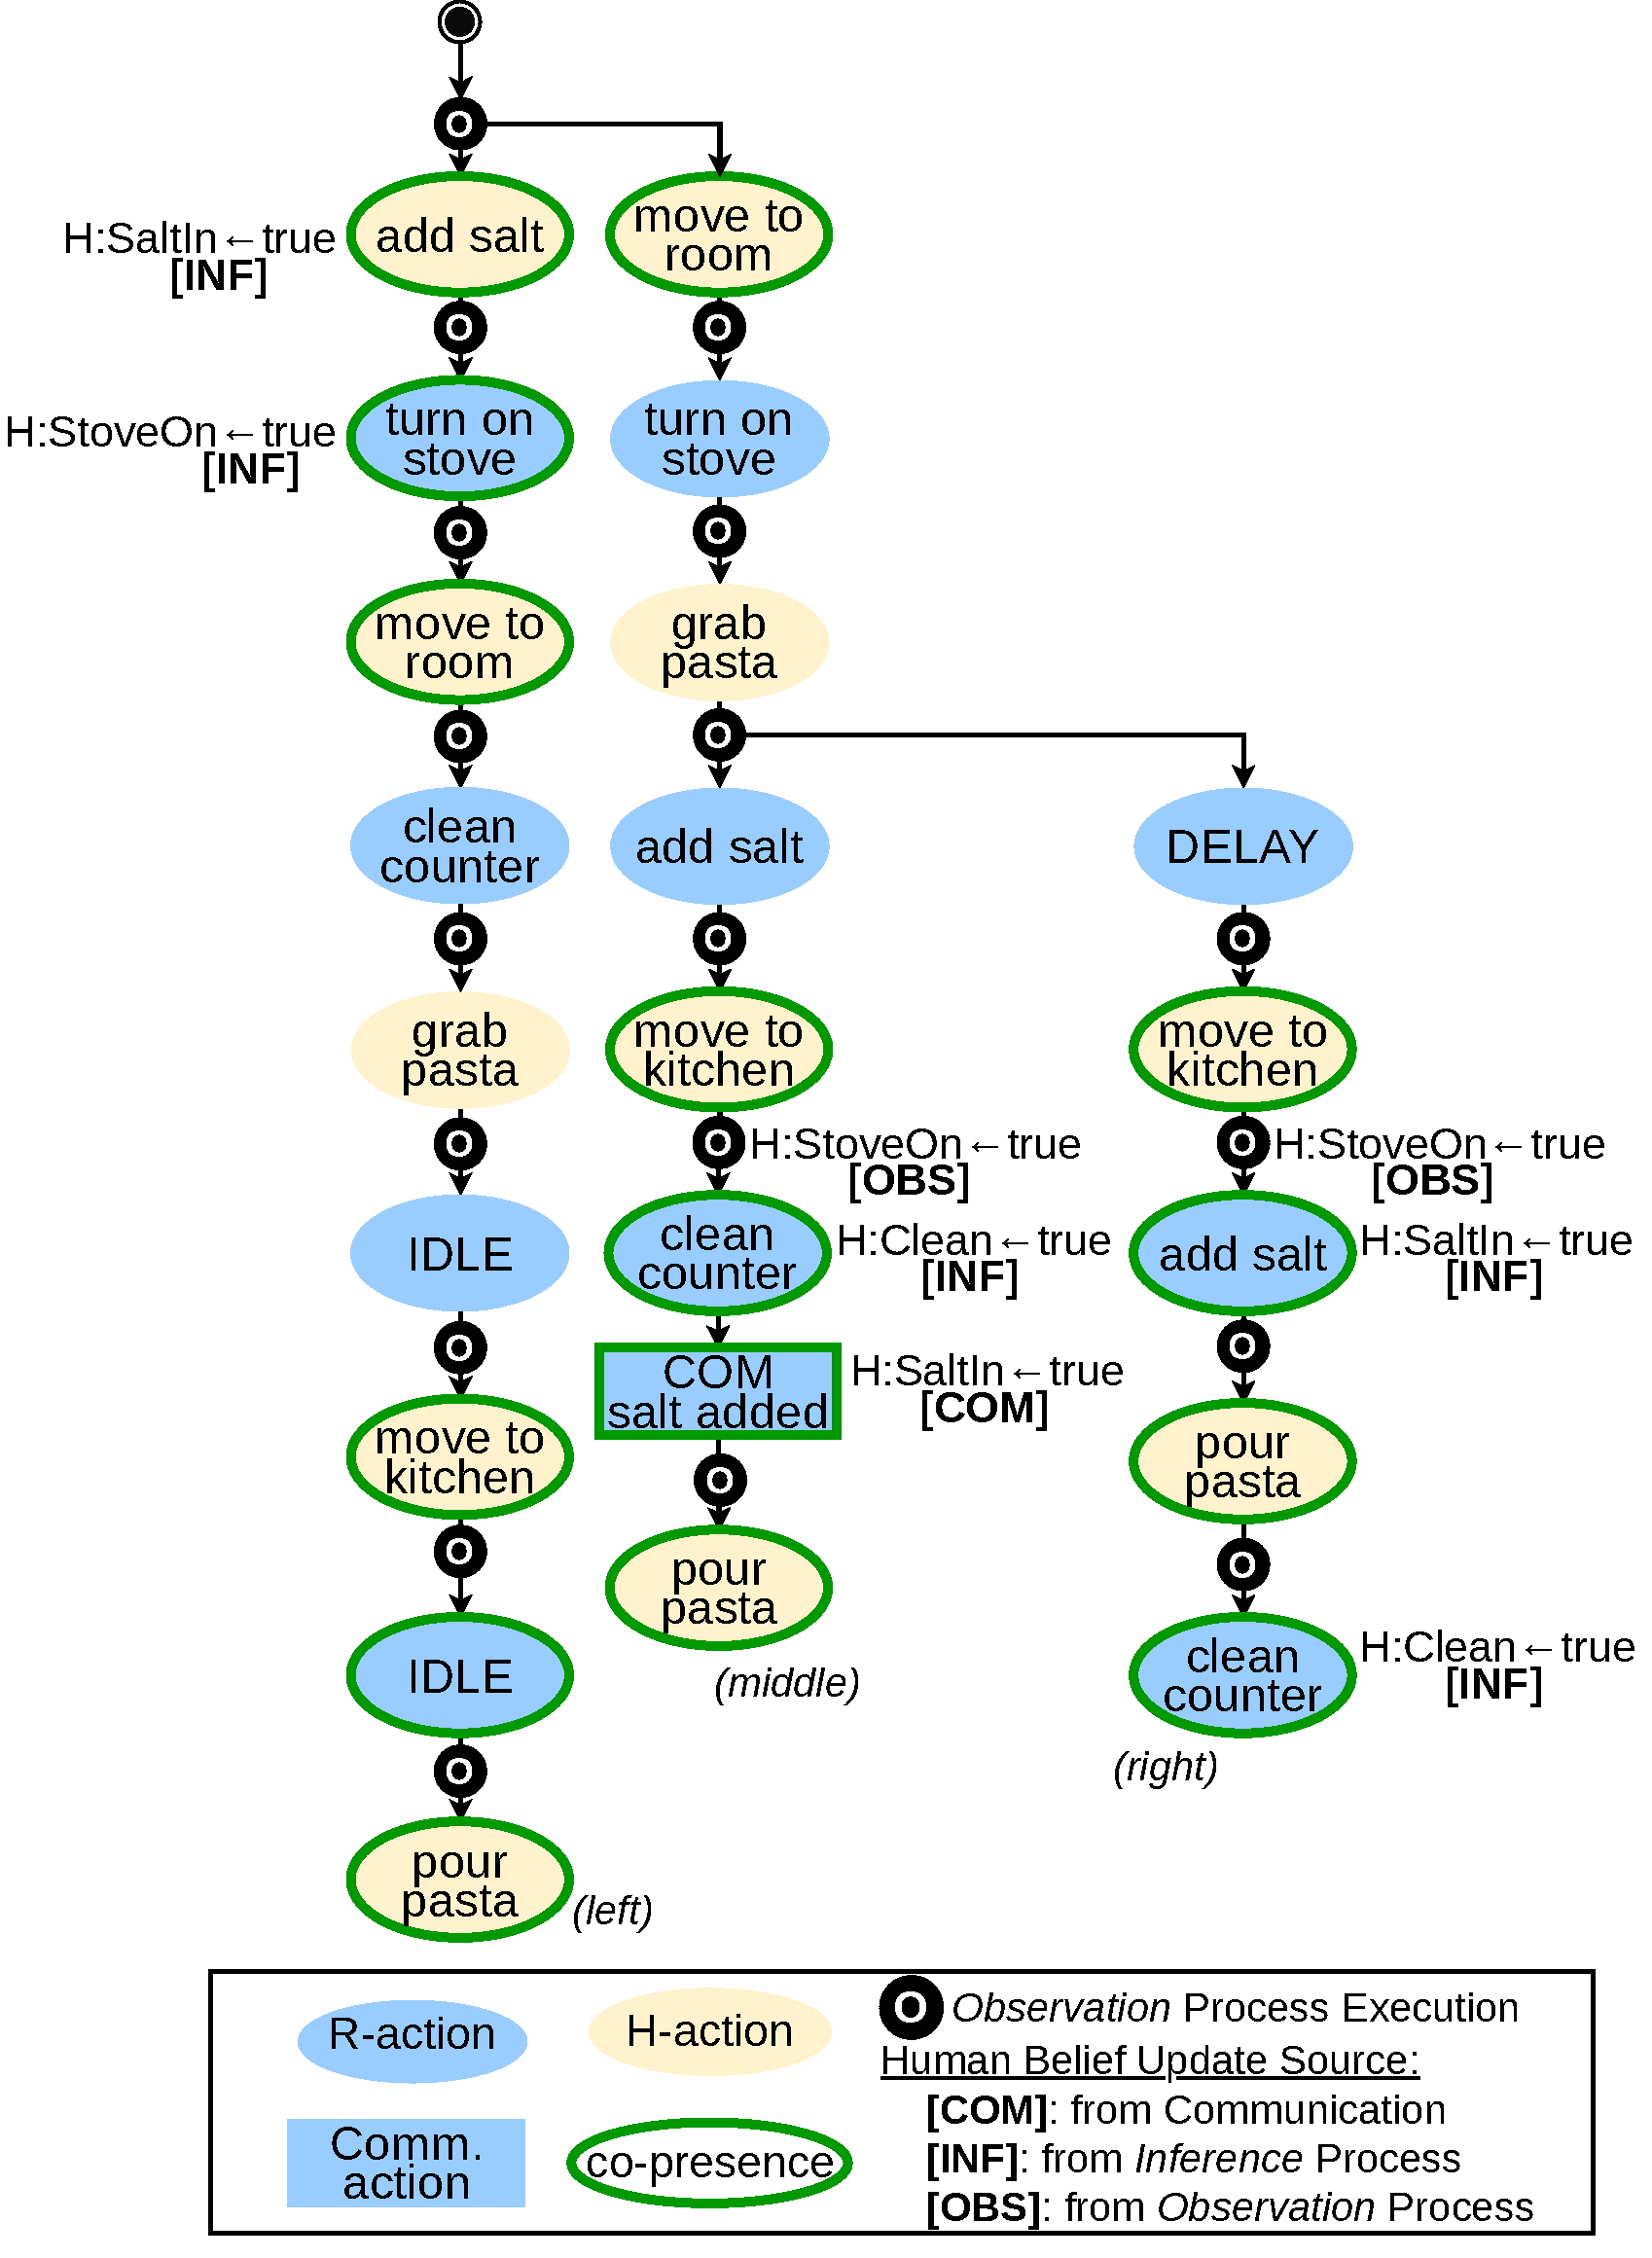
\includegraphics[width=0.65\linewidth]{images/Chapter3/plans.pdf}
    \caption{
    Plan obtained for the cooking scenario. 3 branches. Left: The human starts by adding salt. The only false belief is about \textit{``counterClean''} which is not relevant for the human agent, hence no comm is added. Middle: While the human is away the robot turns on the stove and adds salt, creating 2 false beliefs. 
    Once back, we estimate that the human agent
    will be able to assess the observable fact \textit{``stoveOn''} but not \textit{``saltIn''}. Since the human agent might add salt again due to this false belief, it is relevant and fixed with a communication action. Right: The relevant false belief about \textit{``saltIn''} is avoided by delaying the robot's action until the human is co-present.
    }
    \label{fig:cooking_plan}
\end{figure}

Considering the cooking domain, we discuss in detail the plans obtained with our approach to a problem corresponding to the description given in the introduction. 
I.e., there is no initial human false belief, agents both start in the kitchen, the pasta is in the adjacent room, the stove is off, and there is no salt in the water. The resulting plans are shown in Fig.~\ref{fig:cooking_plan} and their detailed presentation explains how the approach works in practice. 
Since human is uncontrollable and has different possible actions, the plan branches and the robot's actions are different in each case. 

In (\textit{left}) the human first adds salt and then the robot turns on the stove. In both cases, thanks to the inference process, we estimate that the human will be aware of both facts about the salt (\textit{acting}) and the stove (\textit{co-present}). Then while the human is away to fetch the pasta, the robot cleans the counter and since the human isn't co-present their beliefs aren't updated, containing now a false belief. Once back, since \textit{counterClean} is not \textit{observable} the observation process does nothing and the false belief remains. However, this false belief doesn't affect human actions (non-relevant), hence, there is no need to align human beliefs.

In (\textit{middle} and \textit{right}) the human first fetches the pasta by leaving the kitchen. Let's first focus on the (\textit{middle}) trace. The robot turns on the stove and adds salt while the human is away, creating two false beliefs. When returning to the kitchen, the observation process updates the human beliefs with the observable facts located in the kitchen. This fixes the false belief about \textit{stoveOn}. The robot then cleans the counter, observed by the human. 
However, without communication, the human's next action will be either ``add salt'' or ``ask the robot'', but considering the ground truth the human could directly pour the pasta. Hence, the false belief on \textit{saltIn} is relevant and has to be corrected. To do so a communication is inserted in the robot's plan and a ``delay'' branch is created (\textit{right}). 
In this delaying branch, the robot delays the add salt action until the human is co-present in order to make it observed (inference process) by the agent. 
In addition to this implicit communication, like in (\textit{middle}), the human assesses that the stove is on and hence can directly pour the pasta. 
\begin{table}[t]
    \centering
    \vspace{0.1cm}
    \caption
    {
    Success and communication ratio of different approaches. 
    }
    \label{tab:q_results}
    \begin{tabular}{@{}c|c c|| c| c@{}}
    % \begin{tabular}{c|c c|| c}
        \multirow{2}{*}{\textbf{Domain}} & \multicolumn{2}{c||}{\textbf{HATP/EHDA}} & \multicolumn{1}{c|}{\textbf{Only Comm}} & \multicolumn{1}{c}{\textbf{With Delay}}
        \\
        & \multicolumn{1}{c}{\textit{S}} & \multicolumn{1}{c||}{\textit{S I.Div.B.}} & \multicolumn{1}{c|}{\textit{Comm}} & \multicolumn{1}{c}{\textit{Comm}} 
        \\ \cline{1-5}
        \textit{Cooking}    &   18.6\%  &  6.9\%    & 69.5\% & 65.2\%\\
        \textit{Box}        &   25.0\%  & 14.3\%    & 79.7\% & 75.0\%\\
        \textit{Car}        &   12.5\%  & 0.0\%     & 68.8\% & 64.1\%\\
        \hline
        \textbf{Average}    &   18.7\%  & 7.1\%     & 72.6\% & 68.1\%\\
    \end{tabular}
\end{table}

\subsection{Experimental Results and Analysis}

In each domain, the actions and tasks remain the same. So here, a problem is defined by a starting agent ($R$ or $H$) and a pair of initial beliefs ($val^R_0, val^H_ 0$).
Initial ground truth ($val_0 \Leftrightarrow val^R_0$) is defined by setting each state variable to an initial value. But, 5 selected state variables can be set to 2 possible values instead of 1. Among these selected ones, 3 can diverge in human belief. This generates 256 pairs of initial beliefs where 12.5\% of them include initially aligned beliefs. Then, considering the starting agent, we obtain 512 problems for each domain. 
Each of the 1536 generated problems has been solved by HATP/EHDA, by \textit{our approach} using first \textit{only communication} and then using also \textit{delay}.
The obtained quantitative results appear in TABLE~\ref{tab:q_results}.
 
The overall success rate ($S$) and the one for initially diverging beliefs ($S I.Div.B.$) are shown for the HATP/EHDA solver. As expected, this solver always finds legal plans when dealing with initially aligned beliefs, but the low value of $S I.Div.B.$ reflects how poorly it handles belief divergences without specifically designed action models.
Our approach always finds legal plans so we omitted its success rates in the last two columns, and we can say that it solves a broader class of problems.

Furthermore, considering the initially diverging beliefs and the divergences created along the planning process, more than $87.5\%$ of all problems involve belief divergences. 
However, when using only verbal communication, only $72.6\%$ of the generated plans include communication actions.
This means that \textit{our approach} communicates only when necessary, and not systematically. 
The amount of communication is even reduced to $68.1\%$ when delaying actions. In the latter case, only delayed branches that do not imply the human to wait are kept. 

%%% SECTION %%%%%%%%%%%%%%%%%%%%%%%%%%%%%%%%%%%%%%%%%%%%%%%%%%%%
\section{Discussion and Limitations}

The underlying scheme allows just a single agent to execute a \textit{``real''} action at a time. 
However, a post-process can allow the execution of actions concurrently~\cite{CrosbyJR14}, however, note that the domain modeler has modeled $\mathcal{P}_{rh}$ as a sequential joint task. 
Parallelism is not considered in the current modeling and planning process, which limits the potential for concurrent executions. However, we are working on extending the framework to enable systematic planning with concurrent actions, aligning with~\cite{ShekharB20}.

We believe our modeling-level SA proposals could fit in any other planning approach framing multi-party systems having one controllable agent while can only hypothesize remaining agents' behaviors (e.g., human-centered AI).

Agents' SA models cannot simply refute a false belief, they can only assess new true facts to correct them.
E.g., assume the human \textit{wrongly} believes that the pasta is in \textsf{kitchen}. The SA does not help refute this when the agent is in \textsf{kitchen}
because appropriate knowledge reasoning w.r.t. \textit{NotAt(Pasta)} in \textsf{kitchen} is not taken into account.  
However, such issues do not affect the completeness and, if necessary, our approach \textit{tackles} such cases as relevant false beliefs.

We have planned a user study for the future to conform our framework with reality and validate the approach.

We discussed earlier that DEL knowledge representation is more expressive and flexible, and can handle uncertainty. However, it requires an augmented action schema to accurately maintain each agent's beliefs.
Think of a specification for \textit{``move''} action manually listing all the environmental facts to be observed by an agent for managing their beliefs. In our case, it is implicitly maintained within a state.

We can consider running a set of rules (e.g., \textit{graph-based ontology}) to bring new interesting facts in the state based on a set of known facts. We believe that this aspect opens up new possibilities in the future to integrate human-aware collaborative planning and ontology.

%%% SECTION %%%%%%%%%%%%%%%%%%%%%%%%%%%%%%%%%%%%%%%%%%%%%%%%%%%%
\section{Conclusion}

We propose an extension to a Human-Aware Task Planner called HATP/EHDA. 
The planner plans and implicitly coordinates the robot's actions with all estimated possible human (uncontrollable) behaviors that are then emulated to generate a new state.
Our extension and contribution are, first, to integrate a \textit{Situation Assessment} based reasoning system in the planner. This allows for maintaining distinct agents' beliefs based on what they can/should observe.
Compared to existing epistemic planners, this simplifies the action descriptions by focusing on their effects on the world, and not how they influence each agent's beliefs.
In addition, we propose to detect false human beliefs and tackle only the necessary ones in a principled way. First, we propose minimal and proactive explicit communication. Second, when pertinent, 
we propose an implicit communication by postponing the non-observed robot action until the human is co-present to observe it.  

The relevance of false belief, when to optimally communicate and parallelization are interesting future works, and we aim at conducting a user study to validate the benefits of the proactive robot behavior that our approach permits. 
\ifdefined\included
\else
\setcounter{chapter}{3} %% Numéro du chapitre précédent ;)
\dominitoc
\faketableofcontents
\fi

\chapter{Modeling and Planning for Concurrent and Compliant Joint Action Execution}
\chaptermark{Concurrent and Compliant Joint Action Execution}
\label{chap:4}
\minitoc

\chapabstract{This chapter presents my second main contribution, proposing a new human-aware task planning approach based on a step-based model of compliant and concurrent joint action. The approach's description is supported by empirical results proving its effectiveness in terms of the latitude of choice given to the human and the satisfaction of their internal preferences. We further validated this by developing an interactive simulator used for a user study, described in the following chapters.}

\section{Introduction}

\textit{From HRI paper}

In the context of HRC for a shared task~\cite{selvaggio2021autonomy}, we believe, based on the literature on joint action~\cite{sebanz_2006joint,sebanz-2009,clodic-2017,gordon-2023}, that the key towards a seamless interaction is, to consider the human as an uncontrollable agent and to be fully and concurrently compliant with them. 
The human should not be dictated which action they must perform, as in~\cite{roncone2017transparent,buisan_hatpehda_icra}, and the robot must comply with possible human decisions and actions during execution.

To collaborate with such humans with their (hidden) preferences, one can devise an online planning scheme coupled with a plan executor. 
However, in order to maintain real-time performance, online planning generally keeps a restricted horizon. 
Therefore, decisions taken online may lead to a dead end or may not lead to an optimal solution. 
Offline planning overcomes these issues. 

We propose a new \textit{offline} task planner which extends an existing human-aware planning system addressed in~\cite{buisan_hatpehda_icra}. 
The new planner is designed to take into account a \textit{Model of Execution}, which is in the form of an automaton and mainly inspired by the joint actions schemes. 
The model captures humans' latitude in their decisions. 
The planner's output is the robot's behavioral policy, which describes the robot's action in a state such that the action is congruent and compliant with the human's decision in this state and their (estimated) preferences, and that it is also legal to be executed in parallel. 
Our framework also allows humans to share their (new) preferences at any time during execution while the robot's policy is adapted online to that. 
In addition, our approach considers social signals to enhance execution by minimizing uncertainties. Both humans and robots issue signals to clarify situations such as performing an action, waiting for the other agent's necessary actions, or indicating a desire to remain passive.

In this chapter, we discuss relevant related work before describing the joint action model of execution that is central to our approach. 
We then describe the task planning problem and then introduce our novel framework. 
The following two sections to that, explain how the robot policy is generated by a three-step process: \textit{exploration}, \textit{characterization}, and \textit{generation}. 
We empirically evaluated our approach in simulation. With a BlocksWorld scenario, we show how our approach can effectively produce a concurrent robot behavior that is compliant with human online decisions and preferences.  

\section{Related works}

\textit{From HRI paper}

There have been a few attempts to cater to concurrent execution, but they deal with explicit time to manage concurrency~\cite{CirilloKS09a,kockemann2014grandpa}. 
In~\cite{CirilloKS09}, the robot does not plan actions for humans but forecasts their actions/plans from their activities and bases its own decision on the distribution of possible human plans. Here robots can perform actions concurrently, estimating/managing the completion time of the agents' actions carefully. 
We can see the human activity recognition part as a form of our \textit{identification (ID)} process of the automaton used. The robot needs such a plan/goal recognition technique to be compliant with the human's decisions. 
But, unlike ours, they do not consider an explicit shared goal among the agents, and hence humans are not concerned with stuff robots might be interested in during collaboration, e.g., giving signals to be passive. 
We believe that a shared goal creates a different context in HRC than the robot just being compliant with an estimated human's goals/plans. 
Moreover, we claim that dealing with concurrent actions is inevitable in planning even if actions are instantaneous, to effectively deal with multiple agent systems~\cite{CrosbyJR14,ShekharB20}, especially if there is a human operator involved like in our case. 
We extend HATP/EHDA~\cite{buisan_hatpehda_icra} to demonstrate that.

In another work, both \textit{recognition} and \textit{adaptation} take place simultaneously and comprehensively~\cite{levine2014concurrent}. 
It deals with action scheduling of an already generated contingent plan comprising human's and robot's actions. 
It outputs schedules for the robot actions that can execute concurrently but to do that explicit temporal constraints are considered. 

Ramachandruni, Kent, and Chernova (2023)~\cite{RAMACHANDRUNI2023} propose a communication free human-robot collaborative approach for an adaptive execution of multi-step tasks. 
In their approach, the robot observes and supports human decisions, actively selecting actions to optimize collaborative task efficiency. 
Unlike our approach, they introduce an extended collaborative HTN representation with role assignment for planning and state tracking during execution, which is more in line with~\cite{roncone2017transparent}. 
In contrast, we employ two distinct HTNs for robot and human capabilities and use an AND/OR tree for exploration and execution tracking. While their online planning may enhance scalability, optimality is not guaranteed. 
Also, our scheme accommodates both verbal and non-verbal communication, allowing the human to express preferences that update the robot policy online. 

\section{Model of Concurrent Joint Action Execution}

    \subsection{Rationale and Example}



Our task planning approach uses a model of execution to improve the fluency and amenability of HRC. 
This model is in the form of an execution controller and is based on several key notions and mechanisms borrowed from studies on joint actions~\cite{Sebanz_2016,kourtis2014attention}, and adapted to Human-Robot Joint Action~\cite{clodic-2017,curioni-2019}.
The key idea is that co-acting agents co-represent the shared task context and integrate task components of their co-actors into their own task representation~\cite{Schmitz-2017, Yamaguchi-19}. Also, coordination and role distribution rely strongly on reciprocal information flow, e.g., social signals~\cite{curioni-2019}, prediction of other's next action~\cite{luke-2018}.

Our proposed execution model is implemented on a robot that co-acts with a human, integrating explicit representation and exploration of the task representations for the robot and for the human. 
It also identifies precisely how reciprocal information flow is used in task execution (detecting and interpreting human actions, signals produced by the robot while acting, and also when the robot waits for human actions or their signals).

Another essential question is the criteria for choosing the next action, or more globally, how to share the load between the two co-actors. The choice depends on the context and actors' preferences~\cite{Gombolay-2015, Strachan-2020, Curioni-2022}. 
Concerning the case when one actor is a robot, we think it is important to provide a standard default behavior of the robot where the robot does its best to reduce human load but still leaves full latitude to act whenever humans want. 
Our scheme provides this ability and also allows humans to inform about their preferences at any moment.

\begin{figure}
    \center
    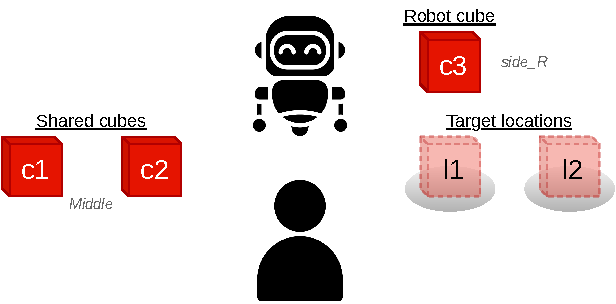
\includegraphics{Chapter4/example_conflict_pick.pdf}
    \caption{Example of conflict for a concurrent joint action. 
    Shared cubes, \emph{c1} and \emph{c2}, can be picked up by both agents and only the robot can pick \emph{c3}. 
    Agents can simulateously pick up both shared cubes, but they must coordinate their actions otherwise they might conflictingly try to pick the same cube. 
    Similarly, another coordination is required to avoid placement conflicts between locations \emph{l1} and \emph{l2}.
    However, notice that the robot can pick \emph{c3} without any risk of conflicts with the human action.}
    \label{fig:conflict_pick}
\end{figure}

To better understand the problem we are trying to solve, let's consider an example where concurrent agent's actions can be conflicting. This example consisting in a simple pick and place task is depicted in fig~\ref{fig:conflict_pick}. The human and the robot have to pick cubes, \emph{c1} and \emph{c2}, that both can reach. 
The cubes can be picked up simulateously unless the agents try to pick the same cube, which causes conflicts between their actions. As a result, despite being executable in parallel, the actions are interdependent. Thus, the agents must coordinate their actions for a smooth execution.
A similar coordination must happen when placing the cubes to avoid conflicts between \emph{l1} and \emph{l2}.
However, a third cube \emph{c3} is present and can only be picked up by the robot. The robot can pick \emph{c3} without any risk of conflicts with the human action. 

This example illustrates the need of coodination even for simple tasks. It also shows that considering possible conflicts can also be a criterion to optimize. Thus, the best robot action might be to pick up \emph{c3} instead of one of the shared cubes to avoid potential conflicts, even if \emph{c3} is more distant and more costly to pick than \emph{c1} and \emph{c2}.
This example also highlight the relevance of exploring several possible executions of concurrent actions while planning to anticipate and evaluate such situations and produce a robust, compliant and efficient robot policy. This is why, based on joint action literature, we formulated a model of concurrent joint action execution described below that will guide our planning search.

\subsection{Abstracted Joint Action Model for Planning}

\begin{figure}
    \centering
    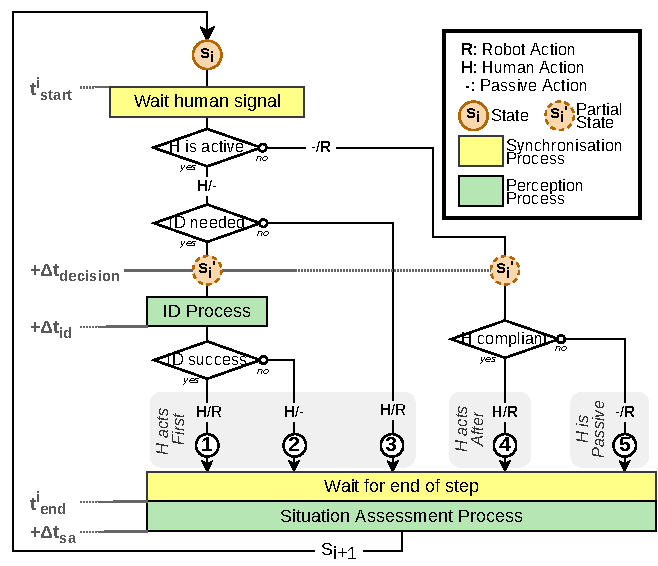
\includegraphics[width=0.8\linewidth]{Chapter4/simplified_automaton.pdf}
    \caption{
    Abstracted Model of Execution in the form of an automaton run by the robot. It captures the latitude of uncontrollable humans in their actions and guides our task-planning approach.
    In this paradigm, the two agents can act concurrently but one is always compliant with the other's decision to act.
    Here, the human is always free to decide whether to start acting first, or after the robot, or not to act at all.
    To be compliant, the robot attempts to identify human decisions using perception and situation assessment as well as possible collaborative human signaling acts (e.g., gestures or speech).
    }
    \label{fig:simplified_model_exec}
\end{figure}

% Full page figure formats w/r line of caption:
% - 5 lines = 210x294 ratio
% - 4 lines = 210x301 ratio
% - 3 lines = 210x308 ratio

The model of execution we formulated, depicted in fig~\ref{fig:simplified_model_exec}, is inspired by joint action literature and describe the agent's coordination during execution. It comprises synhcronisation and perception processes based on social signals exchanged between the agents such as starting an action (arm motion), hand gestures, or verbal communication. In this section is presented a simplified and abstracted version of this model that suffice to guide our planning framework. A complete version which explictely models the human behavior and exhanged signals is provided in the next chapter and used to supervise the execution of the produced robot policy.  


% \textbf{TODO: add numbered marks in the figure to refer to easily for description, also describe the conditions: H is active, etc...}

The model describes the possible transitions from a given state to another, step by step. The robot always informs the human about the beginning of a step and then wait for their decision by looking at social cues. This waiting process is represented by the top yellow rectangle in the figure. This human decision can either be to start acting or to be passive. Hence, the robot always let the human first decide which action they want to perform, including the choice to be passive. This decision is detected with perception by tracking social cues such as human motions and hand gestures.

The diamond shapes below the first synchronization process are conditions, driving the automaton into different branches depending on specific conditions. First, we differenciate the cases where the human is passive or not (``H is active''). 
Ihe case where the human is performing an action, the `yes' branch, we first check if the human action must be identified or not. Indeed, so far only the fact that the human is acting is known, but not yet which particular action they are performing. 
To avoid potential conflicts, we consider that there is no need to identify the human action if the best robot action does not depend on the human decision. For instance, consider in the cube picking example presented in figure \ref{fig:conflict_pick} that the cube \emph{c3} is easier to pick and place for the robot than the two other one. Thus, regardless of which cube the human picks, the robot should pick \emph{c3}, its best action does not depend on the human decision. In such case, there is no need to idenfiy their action. However, if \emph{c3} is effectively harder to place than \emph{c1} and \emph{c2}, the robot must first identify which cube the human is grabbing to pick the other one. As a result, the model differenciate the cases where the human action must be identified (``ID needed'') or not. If not, then the robot can directly start acting (branch 3). Otherwise, the Identification (ID) process is executed and may either be successful (``ID success'') or not. If not, to avoid any potential conflict, we decided that the robot should remain passive (branch 2). If the human action has been successfully identified then the robot can perform concurrently the best corresponding action (branch 1).

In the case where the human decided to be passive, the robot should start acting. 
However, while the robot is acting, we consider that the human is free to either remain passive until the next step (branch 5) or to ``change their mind'' and start acting (branch 4).
This is represented by the diamond shape ``H compliant''. In the case where the human decides to start acting after the robot started, the human can only perform actions that are not conflicting with the already started robot action. Note that this case can be seen as a way for the human to let the robot decide and then comply with the robot's decision. Still, the human decided to let the robot decide, thus, the human is given as much latitude of choice as possible.

Overall, at every step of the execution, the human is free to decide: 1) to start performing any feasible action, the robot will comply with this decision; 2) to let the robot decide and act first, and then purposely we compliant with the robot; 3) to be passive and let the robot act alone.

When both agents finish their actions, the step is considered as \textit{``over''}. This synchronization is represented by the bottom yellow rectangle ``Wait for end of step''. Then, a Situation Assessment Process is executed to assess the new world state ($s_{i+1}$), which is the result of the concurrent actions being executed in the state $s_i$. Once the next state is identified, the automaton repeats until the task is solved and a goal state is reached.

Note that if for any reason both agents are passive during a step, then the state is unchanged and the step is repeated. 

%%%%%%%%%%%%%%%%%%%%%%

% Let's describe this simplified model in the form of an automaton on which on planning algorithm is based on.
% In a state, a human decision can result in one of three outcomes.
% First, the human can choose to act first (\textit{left~subtree}).
% If the robot's best action is not in conflict with the human action (e.g., \textit{pick~C}), the robot can safely perform this action concurrently with the human operator (\textit{branch~3}).
% However, if the robot's best action is either \textit{pick~A} or \textit{pick~B}, the human action must be identified first with a subroutine in order to be compliant with it.
% If this subroutine is successful the robot can perform any action which is congruent with the identified human action (\textit{branch~1}). 
% This includes the robot's choice to be \textit{passive} and let the human act alone. 
% However, if the robot is unable to identify the human action, it must remain passive in order to avoid potential conflicts (\textit{branch~2}). 
% Then, the human can either decide to be \textit{passive} or to act after the robot (\textit{right~subtree}). 
% In both cases, the human is \textit{passive} at the beginning, making the robot to start performing alone a feasible action. 
% While the robot is acting, the human is free to remain \textit{passive} until the next step (\textit{branch~5}) or to choose a congruent action to act concurrently (\textit{branch~4}). 
% As a result, the human can always choose to 1) act first, 2) act after the robot, or 3) not act at all. 
% The robot will always be compliant with these online human decisions.

% When both agents finish their actions, the step is considered as \textit{``over''}. 
% Then, another subroutine assesses the new world state ($s_{i+1}$), which is the result of the concurrent actions being executed in the state $s_i$, before repeating the whole process until the task is solved.

% Note that if both agents are passive (the human decides to be passive when the robot cannot act) then the step is repeated. 

\section{Problem specification + solution}

    \subsection{Problem}

Belief divergences are out of the scope of this particular work. Hence, for simplicity reasons, we consider the two beliefs (robot and estimated human ones) as always aligned, and they are represented as a unique world state. However, we are convinced that this work could be adapted easily to consider the two distinct beliefs.

The problem is specified as shown here \ref{sec:problem_spec} in Chapter~\ref{chap:2}. For simplication purposes, in this contribution, no belief divergence are considered. Therefore, the two agents beliefs are always aligned and initialized with a same initial world state using state variables. Then, distinct human and robot action models are described with HTNs and distinct human and robot initial agendas are provided comprising a shared task to accomplish. 

\subsection{Solution}

\begin{figure}[h]
    \centering
    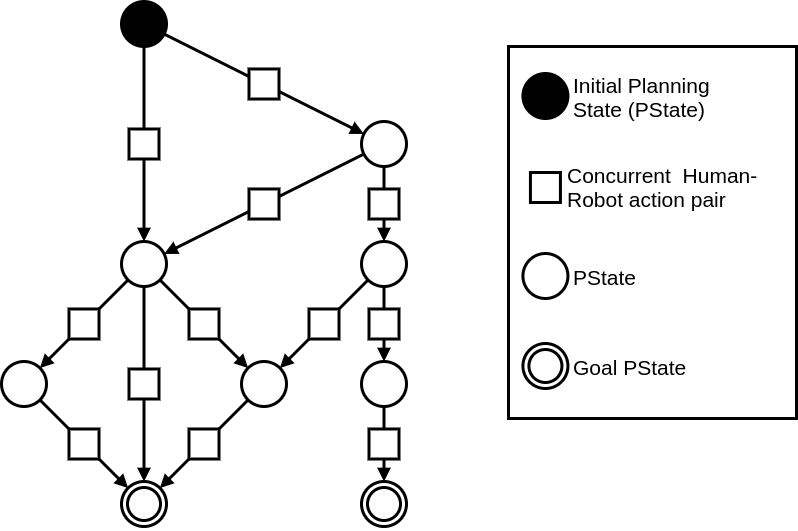
\includegraphics[width=0.7\linewidth]{Chapter4/solution_graph.png}
    \caption{Directed acyclic solution graph}
    \label{fig:solution_graph}
\end{figure}

A Planning state, referred as p-state, corresponds to a state in which the planning problem is while progressing toward a solution. A p-state contains the current world state (aligned beliefs of the agents) and the respective agenda of the human and the robot. Thus, keep in mind that p-states are very different from world states.
The initial p-state is formed using the initial human-robot agendas and the initial world state given in the problem specification. P-states are connected with each other through concurrent pairs of human-robot actions. Note that we consider passive actions, hence, there may be only one active agent in a pair if concurrent human-robot actions. A goal p-state is characterized by a world state satisfying given goal conditions and by empty agendas.
The exploration produces a Directed Acyclic Graph (DAG), referred as the search graph, from the initial p-state to several goal p-states through sequences of concurrent action pairs. Thus, any path from the root to a leaf is a possible plan. Once the exploration done, search graph computed, another process extract the optimal robot policy from the graph. In the manner of an AND-OR tree, this policy indicates for all p-states the best concurrent robot action (OR node) to execute to be compliant with any possible human action (AND node).


Clarification of the directed acyclic graph. Nodes represent p-states and are connected with each other through directed edges representing human-robot concurrent action pairs. However, for practical reasons action pairs are considered as nodes of the graph having only one parent p-state node and one child p-state node. Consider that each directed edge between two p-state have one unique intermediate action pair node. The graph has one root node (no parent) which is the initial p-state. All leaf nodes (no children) represent a goal p-state. 

It is one of our design choice to do not consider explicit action costs and perform an exhaustive offline search to produce this search graph in order to solve a problem. Since the policy generation is very quick it allows generating and updating the robot policy online according to human feedbacks. 


\begin{figure}
    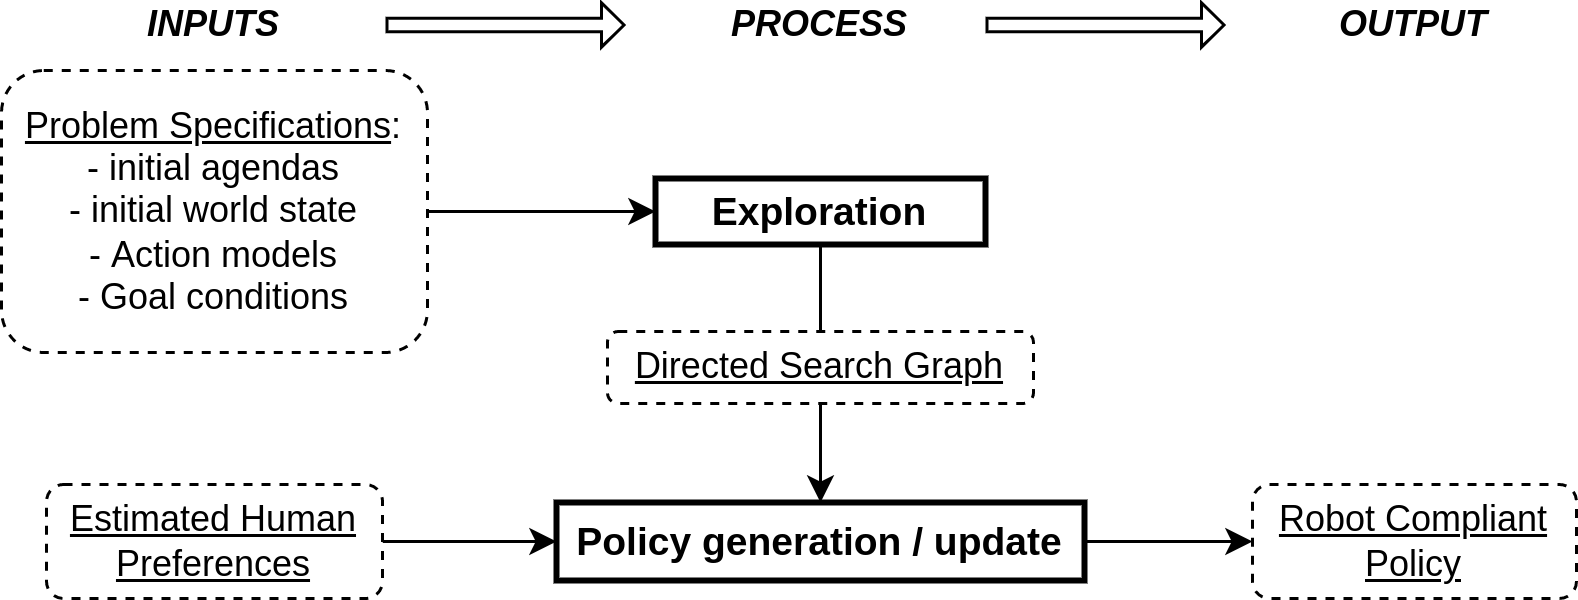
\includegraphics[width=\linewidth]{Chapter4/overall_process.png}
    \caption{Overall planning process}
    \label{fig:overall_process}
\end{figure}

\section{Exploration}

This section details how the exploration happens, and thus, how the search graph is generated. This requires several sub-process which are each detailed here. First, the overall exploration process is presented, and next subsections provide details on the sub-processes mentioned in the overall process.

    \subsection{Overall process}

We keep track of the p-state to explore, and this set is being initialized with the initial p-state. Then, until the set is empty we select one and explore it.
First, from this selected p-state, every possible concurrent human-robot action pairs are computed considering both agendas, the world state and reasoning on the compatibility of the actions in terms of preconditions and effects. This process requires several sub-steps and is detailed later. Thus, we obtain several action pairs leading to the same amount of new p-states (with updated world state and agendas).
Second, we check if any of the newly created p-state are similar to any existing p-state. If so, we can "merge" them to avoid redundant computations. To do so, we basically keep track of the unique p-state already checked and for each new p-state we check if it is similar to one of the already checked one. 
If not, the new p-state is added to the set of already checked p-states. 
If a similar one is found, the new p-state is deleted and the action pair leading to it is connected to the existing p-state instead.
Eventually, the remaining new p-states are added to the set of p-states to explore. 
When the set of p-states to explore is empty then the exploration is over and the graph obtained corresponds to the "search graph" where any path from the initial p-state to a leaf corresponds to a possible execution trace / plan.

    \subsection{Compute next agent actions}

From a p-state, more precisely from a world state and an agenda, we can estimate what are the next action an agent is likely to perform. Doing so is referred as the refinement process. To do so we use the corresponding action model in the form of an HTN. Here the agendas are considered as list of abstract or primitive task, where primitive task can be executed (actions), and abstract ones can be decomposed into several others subtasks. 
The refinement process consists in applying applicable methods of the first task of the agenda until it is primitive. When several methods are applicable they are all applied in a distinct refinement trace.
Eventually, for each different sequence of applied method we obtain a new agenda starting with a primitive task. For each such primitive task we create a copy of the world state contained in the given p-state, and we applied the correspond action, updating the world state. 
Hence, for each possible action a new p-state is created with the refined agent agenda, the unchanged other's agenda and the updated world state. 
Note that this process can "generate" default passive actions in several cases. First, when an agent's agenda is empty an \textit{IDLE} passive action is inserted as the first primitive task in the agenda. This means that the agent has nothing to do and thus is likely to remain passive. Either when there are no applicable methods or when the primitive task is not applicable then a \textit{WAIT} passive action is inserted. This means that the agent has still something to do but cannot do it currently. Note that when computing the concurrent pairs of action we also add the \textit{PASS} action which corresponds to the agent being voluntary passive, despite having something to do. Note also that these different passive action types just help to better understand the generated plans, but they are treated equally / similarly in the planning process.

    \subsection{Concurrent action pairs computation}

This sub-process computes from a given p-state all possible concurrent action pairs that may be executed. It is based on the previously described refinement process. This main objective of this sub-process is to identify the next actions the agents are likely to perform to reach the goal and identify which of them can be executed in parallel. The classical way to do such reasoning is by analyzing the preconditions and effects of the two actions and determine if there are conflicts between them, e.g., the effects of the first action makes the preconditions of the other false.
However, our current python implementation of the planner is convenient but has no "explicit" preconditions and effects. Everything is defined through python function. The effects of an action are a function with a world state as input and returns the updated world state. Action preconditions are functions with a world state as input and return a boolean. And methods (of an associated abstract task) are functions with world state as input and return a list of tasks to update the agenda with. Methods also have preconditions working similarly then action preconditions. 
Hence, it's challenging to extract the explicit effects and preconditions of an action. That is why we decided to rely on an assumption to check the compatibility of concurrent actions. 
We consider the following in a given state. 
If action 1 and action 2 can be sequentially performed in both orders (1$\rightarrow$2 and 2$\rightarrow$1). Then we can assume that there are no causal links between the two actions and that they can be performed concurrently. The only care to take are shared resources such as a tool that would only be used during the action, making it available before and after but not during the action. To tackle this issue, shared resources are explicitly declared in the world state and in the action models. Two actions requiring a same shared resource cannot be parallelized.
One benefit the way we check if two actions are mutually exclusive is making the actions estimations a black box. Indeed, we can easily replace the way we estimate the next actions each agent is likely to perform. Especially for the human, we could use a pretrained human activity estimator neural network, or more classical planner like PDDL. 

With the causal principle above in mind, we proceed as follows to compute the possible concurrent action pairs from a given p-state. We start by estimating all possible human actions by refining the human agenda, generating a new p-state for each possible action. For each such p-state we first create an action pair where the robot is passive by inserting a \textit{PASS} robot action. This \textit{PASS} pair is stored among all other "human pass pairs". Second, we refine the robot agenda to obtain all feasible sequences of human then robot actions and their associated p-states. We refer to them as the sequential human starting pairs. In a symmetrical way we compute the sequential robot starting pairs and "robot pass pairs" by starting with the robot then refining the human agenda.

Eventually, every action pair which is present in both the human and robot starting pairs are extracted and added to a set of concurrent action pairs. 
Additionally, here passive action are always parallelizable. Indeed, the only case where this couldn't be the case is when considering "joint actions" requiring the two agents such as lifting a table/object together. For now, such actions are not considered. Thus, the two sets of \textit{PASS} pairs are directly added to the set of concurrent action pairs. 
Lastly, a double passive pair with two PASS is generated and added to the concurrent set. This pair is special since it doesn't update the world nor the agendas, hence, it leads back to the previous p-state without progressing toward the goal. These pairs not need to be explored and help it different ways. First, it helps the execution for instance when only the human can act but decides anyway to pass voluntary. Then the policy will natively stay in the same p-state. Second, it is easy to detect dead-ends which correspond double \textit{WAIT} pairs. In such case, both agent cannot act, due to the lack preconditions for action or decomposing an abstract task, and they remain stuck without solving the task.  
Last, double \textit{IDLE} pairs indicates that both agendas are empty and thus that the task should have been solved. 

The obtained set of concurrent action pairs corresponds to all possible concurrent action that the human and the robot can execute in parallel in the initially given p-state. Each possible pair leads to a new p-state with updated agendas and world state, creating a tree structure. 

    \subsection{Merging p-states}

Although the tree structure produced by the process described above is complete and sound, it is inefficient and scales badly. Indeed, during the exploration we are likely to encounter several times similar p-states. For instance, consider an action pair where both the human and robot are active leading to a new p-state, one branch. Now, consider a first action pair where only the human is active, and a second where only the robot is active. Performing those two last pairs in both orders creates two other branches. However, even though the trace is different, the three p-states are identical (same world state and agendas) and it's highly redundant to explore independently each of them. That is why after each computation of the concurrent action pairs we check if any of the newly generated p-state is similar to an existing one, and if so, we connect the corresponding pair to the existing p-state to avoid redundant explorations. Doing so we transform the tree structure into a directed acyclic graph (on the condition that we don't consider double \textit{PASS} cycles). In the manner of a tree, we will refer to nodes without child as leaves nodes, which are goal p-states. Hence, now, each leaf can be reached with several paths. 
When looking for similar existing p-state, we assume that p-states which are parent with the new p-state, directly of not, will necessarily be different, and thus they are excluded. This speeds up the comparison process. 

\section{The Robot Policy}

First of all, as depicted in figure~\ref{fig:and_or}, all children concurrent action pairs of a p-state ($PS / ps_i$) can actually be seen as an AND-OR graph. Since we want to preserve the latitude of choice the human have at execution, each possible human choice of action is considered as an AND edge and leads to a partial p-state ($PS' / ps_i^j$). And from a partial p-state, each compliant concurrent robot action is considered as an OR edge and leads to another p-state.

Notations: A p-state is referred to as $ps$, and $ps_i$ is the $i$-th p-state. A partial p-state is referred to as $ps'$ and $ps_i^j$ is the $j$-th partial p-state of the $i$-th p-state.

Thus, generating the robot policy $\Pi$ consists in identifying the best concurrent compliant robot action $RA^*$ for each possible human action, or partial p-state $ps_i^j$.

These best concurrent robot actions are determined by aiming to optimally satisfy an estimation of the human preferences regarding the task. Eventually, at execution, the human is free to perform any of the explored action and the robot will accordingly perform an optimal concurrent action to both solve the task and satisfy their estimated preferences.

Hence, before giving more details about the policy itself, we first describe the format of human preferences, how we could estimate them, and what it allows us to do. After, we describe the actual process to generate the robot policy from the search graph using the estimated human preferences


**The robot policy consist in performing the best robot action according to the node and the human action, i.e., robot action stored in the "best compliant" pair corresponding to the human action.
If all "best compliant" pair have the same robot action, the robot can perform as soon as the step stars, otherwise the human action must be identified.**

\begin{figure}
    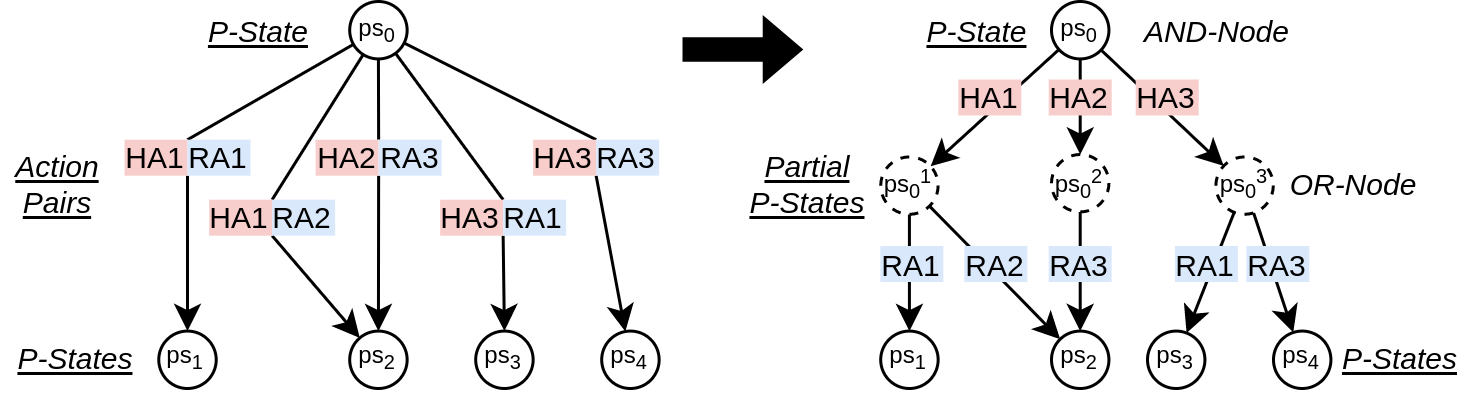
\includegraphics[width=\linewidth]{Chapter4/and_or_tree.png}
    \caption{AND-OR graph representation of the action pairs. 
    The robot policy must be compliant to any decision of the human. Hence, the problem can be seen as an AND-OR graph where for each possible human choice of action (AND node), we must determine the best concurrent robot action among the possible robot actions (OR node).
    }
    \label{fig:and_or}
\end{figure}


    \subsection{Estimated Human preferences}
estimations, format, Discussion(often inaccurate, hence our Approach), consider metrics, is a prioritized sequence of metrics to max or min, allow comparison of metrics

In this approach, instead of trying to minimize action and social costs, which are challenging to estimate accurately and quantitatively, we decided to aim at satisfying an estimation of the human preferences. In a way, the costs are included / covered / reflected in the human preferences. Our approach is to characterize each possible trace with a set of various metrics such as follows:

\begin{itemize}
    \item \textbf{Time of Task Completion}: Time step at which the task if achieved.
    \item \textbf{Time of End of Human Duty}: Time step after which the human can remain passive.
    \item \textbf{Human Effort}: Number of non-passive human action.
    \item \textbf{Global Effort}: Number of non-passive human and robot action.
    \item \textbf{*Passive While Holding}: Number of steps where an agent is passive while holding a cube.
    \item \textbf{*Number of Drop}: Number of times an agent drops cube (place back a cube on the table, not in the stack).
\end{itemize}

Note that general metrics are complemented with additional domain specific metrics (marked with a star *), given in the problem specification. The set of metrics helps to characterize and evaluate each possible plan / trace. However, even if the possible plans are characterized we so far have no way to compare them and find the best one. Doing so requires additional criteria indicating how to prioritize and compare the different metrics.

That's where we consider an estimation of the human preferences to allow us to the plans and which are given by any mean external to our system. The preferences can be estimated or also given, verbally or not. Here, we consider the human preferences in the following form. These preferences are an ordered list of the metrics characterizing the traces. Note that it's not necessary for all metrics in the list above to be present, but only them can appear in the preferences. This ordered list indicates if each metric should be maximized or minimized, and in which order / with which priority. For instance, assuming the preferences aim to minimize all metrics, the best of two given plans is the one with the lowest first metric of the list. If the two plans have equal first metric then we use the second metric, and so on. Here are two arbitrary examples of human preferences trying respectively to finish the task as fast as possible and to minimize the human effort (all metrics are minimized):

TTC - GE - HE - TEH - PWH - ND 

HE - TEH - TTC - GE - PWH - ND 

Note that estimating either human preferences or explicit action and social costs is challenging and is hardly accurate, those are very context dependent and can even vary over time.
Being aware of this, we use the estimated human preferences as a guide for the robot behavior, but we also make sure to be compliant to the human activity to lessen the impact of a wrong estimation. 

    \subsection{Generation}

\begin{figure}
    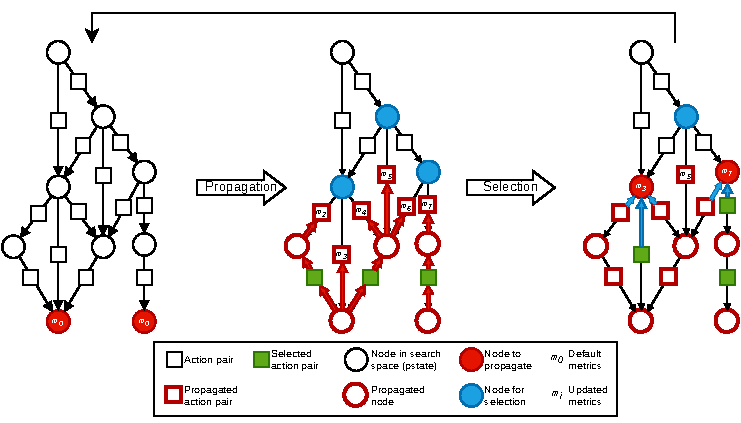
\includegraphics[width=\linewidth]{Chapter4/policy_generation.pdf}
    \caption{\textbf{TODO: show metrics in branches? just small $m_i$ in each branch?} Policy generation process illustration on an arbitrary search graph. Propagation and Merge processes repeat until there are no more p-state/node to propagate nor for selection.}
    \label{fig:policy_generation}
\end{figure}

To generate the robot policy $\Pi$ from the search graph we proceed from the leaves to the root. 
Overall, we progressively compute the set of metrics for each possible trace. When reaching a p-state with several children we compare the metrics of the different traces leading to this node. We are then able to identify the best trace leading to each partial p-state, and the best trace leading the p-state. Each best trace to a partial p-state is used to update the robot policy, and the overall best trace is used to continue propagation the best reachable set of metrics.
This process is achieved by repeating two sub-routines detailed just below, namely: Propagation and Selection. 

\begin{algorithm}
\caption{Policy Generation}\label{alg:policy_generation}
\begin{algorithmic}[1]

\State \textbf{input}: $leafNodes$ \Comment{Set of all leaf p-states from the search graph}
\State $psToPropagate \gets \emptyset$
\State $psForSelection \gets \emptyset$

\State $Initialization(psToPropagate, leafNodes)$

\While{ $psToPropagate \neq \emptyset$ and $psForSelection \neq \emptyset$ }
    \State $Propagation(psToPropagate, psForSelection)$
    \State $Selection(psToPropagate, psForSelection)$
\EndWhile

\end{algorithmic}
\end{algorithm}

    \subsubsection{Format and Initialization}

During this process we compute and store the best reachable set of metrics alternatively in the p-states and in the action pairs. Initially, we store default/null metrics in every leaf p-state. Then we keep track of two types of nodes. First, keep track of the nodes which metrics should be propagated in the next step, those are stored in the set $\{psToPropagate\}$ which is initialized with all leaf p-state nodes. This set is later populated by the Selection sub-routine. Secondly, we keep track of the nodes to that should select among several the best set of metrics, and thus, the best actions to perform. This set is $\{psForSelection\}$ and later is populated by the propagation sub-routine while being emptied by the selection sub-routine. The process is over when the two sets are empty, thus, when they are no more nodes either to propagate nor for selection.

% The default metrics are the following:
% \vspace{-\topsep}
% \begin{itemize}
%     \setlength\itemsep{-0.3em}
%     \item \textbf{Time of Task Completion} $= -1$
%     \item \textbf{Time of End of Human Duty} $= -1$
%     \item \textbf{Human Effort} $= 0$
%     \item \textbf{Global Effort} $= 0$
%     \item \textbf{*Passive While Holding} $= 0$
%     \item \textbf{*Number of Drop} $= 0$
% \end{itemize}

    \subsubsection{Propagation}

The propagation sub-routine is depicted in algorithm~\ref{alg:propagation} and described here. It consists in picking a node to propagate from the set $\{psToPropagate\}$. For each parent action pair of that node we create a copy of the set of metrics of the propagated node and update them according the parent action pair and propagated node. 
The metrics must be cumulative. 

Rules to update the standard metrics are the following \textbf{TODO: TO UPDATE, THERE IS AN OFFSET OF 1 FOR TIME STEP METRICS => should be done by giving the default metrics}:
\vspace{-\topsep}
\begin{itemize}
    \setlength\itemsep{-0.3em}
    \item If the pair is not \textit{IDLE}-\textit{IDLE}, then increment (by 1) \textit{Time of Task Completion}
    \item If the pair is not \textit{IDLE}-\textit{IDLE}, if the human action is passive, and if the current \textit{Human Effort} is zero, then the temporary metric \textit{Number Last Passive Human Action} is incremented.
    \item \textit{Time of End of Human Duty} = \textit{Time of Task Completion} - \textit{Number Last Passive Human Action}.
    \item If human action is not passive, then \textit{Human Effort} and \textit{Global Effort} are incremented.
    \item If robot is not passive, then \textit{Global Effort} is incremented.
\end{itemize}
Rules to updates domain specific metrics, must be provided:
\vspace{-\topsep}
\begin{itemize}
    \setlength\itemsep{-0.3em}
    \item If human action is passive and in child p-state the human is holding a cube, then \textit{Passive While Holding} is incremented.
    \item \textit{(Similarly with the robot)}
    \item If the human action is to drop a cube back on the table, then \textit{Number of Drop} is incremented.
    \item \textit{(Similarly with the robot)}
\end{itemize}

The updated metrics are stored in their corresponding action pair. Then, two cases can occur for each parent action pair with stored metrics, referred as propagated pairs. First, if the parent node of the propagated pair has more than one child then we add this parent node to the set $\{psForSelection\}$. Otherwise, the metrics of the action pair are stored in the parent node which is also added in the set $\{psToPropagate\}$. 
The sub-routine repeats until the set $\{psToPropagate\}$ is empty.

\begin{algorithm}
\caption{Propagation Sub-Routine}\label{alg:propagation}
\begin{algorithmic}[1]

\While{ $psToPropagate \neq \emptyset$ }
    \State $N \in psToPropagate$
    \State $psToPropagate \gets psToPropagate \setminus \{N\}$
    \For{ each $P$ in $N.parents$ }
        \State $P.metrics \gets CopyAndUpdateMetrics(N.metrics, N, P)$
        \If{ $HasOneChild(P.parent)$ }
            \State $P.parent.metrics \gets P.metrics$
            \State $psToPropagate \gets psToPropagate \cup \{P.parent\}$
        \Else
            \State $psForSelection \gets psForSelection \cup \{P.parent\}$
        \EndIf
    \EndFor
\EndWhile

\end{algorithmic}
\end{algorithm}



    \subsubsection{Selection}

Introduce policy notation, p-state and partial p-state (AND-OR tree)

When a node has several children, possible action pairs, then we must evaluate and compare them in order to make the best robot choices and update the policy with them. The evaluation is part is done by the propagation sub-routine. The Selection one checks when robot choices are ready to be made, update the robot policy and prepare the next propagation phase. 

The selection sub-routine is depicted in algorithm~\ref{alg:selection} and described here. It checks every node in the $\{psForSelection\}$ set to know if we are ready to make a choice, i.e., if every child pair of that node has metrics stored in it, has been propagated. 
If not, nothing happens and the node remains in the set.
If so, we are ready to compare the pairs and update the policy. Since we want the human to be free to perform any action, even suboptimal, we must find the best concurrent robot action for each possible human action. The first step is to group/sort/organize the children pairs by similar human action. Then, for each group of pairs, we compare their metrics using the estimated human preferences and identify the best pair of the group, which is marked a ``best compliant pair''. After, all marked pairs are compared the overall best pair is identified and marked as ``best pair''. Eventually, the metrics of the ``best pair'' are stored in the node from $\{psForSelection\}$, the node is removed from the set and added to the other set $\{psToPropagate\}$.

\begin{algorithm}
\caption{Selection Sub-Routine}\label{alg:selection}
\begin{algorithmic}[1]

\For{ each $PS$ in $psForSelection$ }
    \If{ $ReadyForSelection(PS)$ }
        \State $bestPairs \gets \emptyset$
        \For{ each $partialPS$ in $GetPartialPStates(PS)$ }
            \State $pairs \gets GetCorrespondingPairs(partialPS)$
            \State $P \gets IdentifyBestPair(pairs)$ \Comment{Compare metrics and identify best}
            \State $\Pi(partialPS) \gets P.robotAction$
            \State $bestPairs \gets bestPairs \cup \{P\}$
        \EndFor
        \State 
        \State $bestPair \gets IdentifyBestPair(bestPairs)$
        \State 
        \State $PS.metrics \gets bestPair.metrics$
        \State $psForSelection \gets psForSelection \setminus \{PS\}$
        \State $psToPropagate \gets psToPropagate \cup \{PS\}$
    \EndIf
\EndFor

\end{algorithmic}
\end{algorithm}

    \subsubsection{Additional policy updates}

After executing the main process to generate the robot policy $\Pi$, each partial p-state $ps'$ is mapped to a robot action to execute. So, for the robot policy to be executed the partial p-state must be identified at runtime. 
Since, a partial p-state is characterized by the choice of action the human made, this identification is done through the ID process mentioned in the Model of Execution which briefly tries to identify which action the human is starting to execute during a step. However, such identification can be challenging, so we try to avoid it when possible. 

Indeed, for any p-state $ps_i$ from the search graph, if $\forall j, \Pi(ps_i^j) = RA$ with $RA$ being one unique/same robot action, then the best robot action doesn't depend on the human choice. Thus, in such case, the ID process can be avoided, and the policy is complemented as follows $\Pi(ps_i) \gets RA$.

Moreover, we consider cases where the ID process failed to identify the human action, and is noted as $\lambda$. To prevent potential conflicts due to identification failure the policy is updated s.t. $\Pi(\lambda) = PASS$.
Note that in this work we only consider identification failures and not wrong identifications. 

% Note also that, based on the Model of Execution, each step starts when indicated by the robot, but the robot always wait for the human decision before acting. This human decision can either be active, which is easily detected, and if needed the exact human action is identified through the ID process. The human can also decide to be passive. This is detected either by observing the \textit{PASS} signal (hand gesture) or if the human neither act nor make a hand gesture within a defined time-out. Thus, for    
%% PASS always detected ?? actually not needed since not a regular action and if not identfied the TO will be triggered and it's fine. 

If human is passive ? dedicated partial p-state identified after WaitHumanDecision.

    \subsection{Execution}

The execution of the policy stems from the Model of Execution automaton and is depicted in Algorithm~\ref{alg:execution}.

\begin{algorithm}
\caption{Execution of the Robot Policy }\label{alg:execution}
\begin{algorithmic}[1]

\State $ps \gets ps_0$ \Comment{Initial state}
\While{ $ps.children \neq \emptyset$ }
    \State $IndicateStepStarted()$ \Comment{Inform the human}
    \State $WaitHumanDecision()$
    \If{ $ps \in Domain(\Pi)$ } \Comment{If ID not needed}
        \State $Execute(\Pi(ps))$
    \Else
        \If{ $HumanIsPassive()$ } \Comment{Detected by $WaitHumanDecision$}
            \State $Execute(\Pi(ps'))$
        \Else
            \State $idPartialPS \gets IDProcess()$ \Comment{$\in \{\lambda\} \cup \{ps'\}$}
            \State $Execute(\Pi(idPartialPS))$
        \EndIf
    \EndIf
    \State $WaitEndStep()$ \Comment{Human and Robot actions are done}
    \State $ps \gets AssessementProcess()$ \Comment{Identify executed pair, and next $ps$}
\EndWhile

\end{algorithmic}
\end{algorithm}

\section{Empirical Results}
simulation of execution, without durative action

We provide results obtained after simulating symbolically the execution of robot policies produced with our approach, thus without durative actions. 

    \subsection{Simulated Experiment}

The execution is symbolically simulated by running an implemented version of the automaton described in the \textit{model of execution}. This implementation is close to the presented algorithm~\ref{alg:execution} where action execution are mocked and replaced by symbolic and instantaneous actions. [Info on other mocked processes ? ID ? Wait?]
Thus, the current state progresses in the search graph based on the human decision and the produced robot policy before eventually reaching a leaf node indicating that the goal is satisfied. 
We then retrieve which course of action has been executed to then analyze it.

We evaluated our approach in the BlocksWorld domain. Figure~\ref{fig:block_world_domain} shows one problem instance. 
The human and the robot are on two sides of a big table and their shared task is to stack colored cubes as shown in the given goal pattern. 
Initially, all colored cubes are arranged on the table that is divided into three zones: Each agent has a dedicated zone (\textit{RZ} \& \textit{HZ}) and a common zone (\textit{CZ}) is in the middle and accessible for both. 
Each agent can only pick cubes from either their own zone or from \textit{CZ}. 
There is a box in \textit{RZ} in which cubes can be inserted. To pick such cubes the robot must first perform a dedicated action to open the box before being able to use the cubes inside it like the regular ones.


\begin{figure}
    \centering
    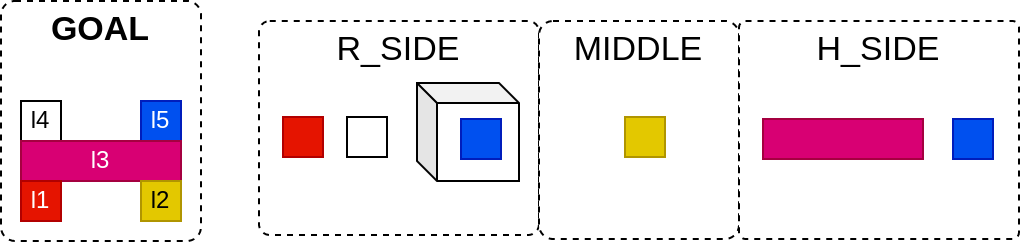
\includegraphics[width=\linewidth]{Chapter4/block_world_domain.png}
    \caption{An instance of the BlocksWorld domain. The ideal plan is strongly influenced by the human desired preferences. For the earliest end of the task, the human prevents using the box. A lazy human will only place the required pink bar from their side. And a human in a hurry will place concurrently the yellow cube to place the pink bar at the earliest and be able to leave.}
    \label{fig:block_world_domain}
\end{figure}


    \subsection{Human behavior and erroneous estimated preferences}

To simulate the human behavior, we consider and define human preferences that produce a human policy in the same manner as for the robot. The produced human policy makes the human always perform the best action regarding their defined preferences. The robot/planner doesn't have access to the human preferences but only to an estimation of them.

In order to evaluate the quality of the executed trace regarding the actual human preferences we compare and rank every possible trace from the search graph, from best to worst. For legibility purposes, we normalize the ranks to obtain a score (H-score) s.t. the trace/plan with the lowest rank has a score of 0.0, while the highest rank corresponds to a score of 1.0. This score represents a quality indicator independent of the instance's size. 
Similarly, we can do the same and acquire the score regarding the robot's estimation of the preferences (R-score). 
Keep in mind that the R-score is an estimation of the actual H-score, and the robot acts in order to maximize its R-score, hoping to maximize as well the H-score.

However, the estimation of the human preferences can be more or less accurate, causing the robot's decisions to differ from what humans would have preferred. Once again, that's why making the robot compliant with human online decisions and actions gives the human more influence over the execution and helps to reach high H-score even when the robot's estimation is incorrect.
Despite the robot trying to maximize its R-score, it's important to note that reaching a low R-score is fine as long as a high H-score is attained.

\begin{figure}
    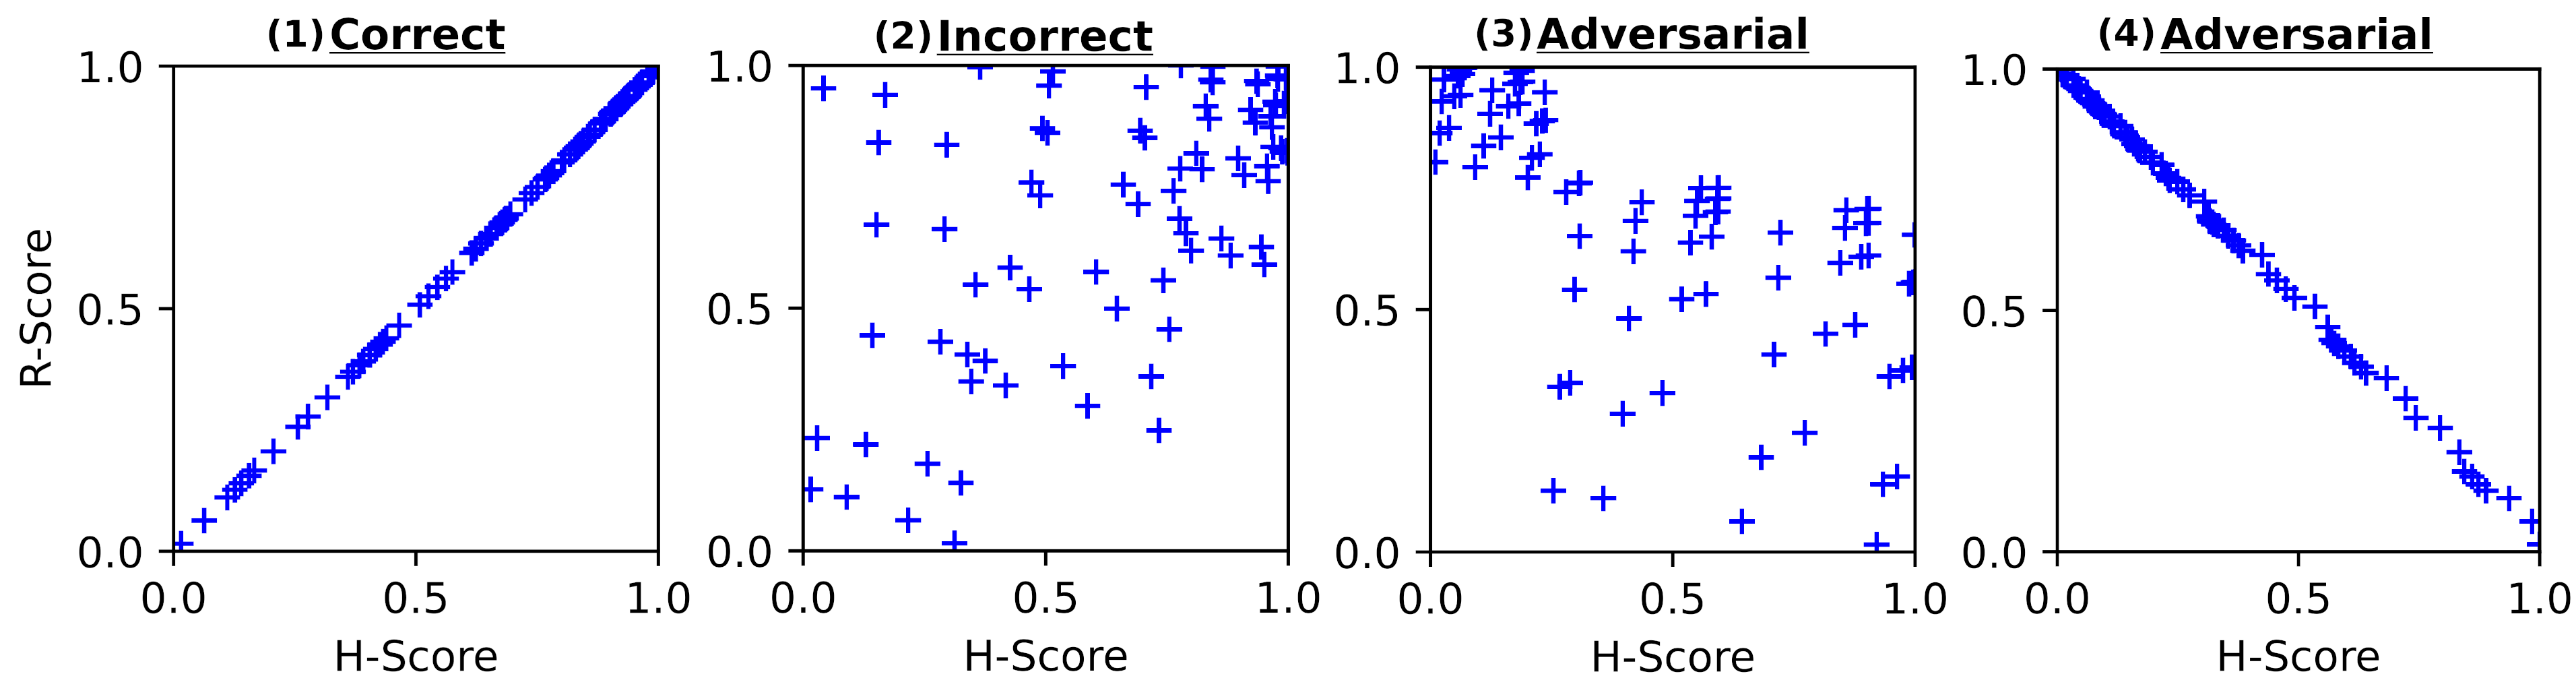
\includegraphics[width=\linewidth]{Chapter4/all_corr.png}
    \caption{
    Correlation between the H-score and R-score according to different robot estimations. Four pairs of human preferences and their estimation are considered. For each pair, all possible traces are plotted as blue crosses according to their H-score and R-score. \textit{(1)} show a correct estimation while the others show incorrect estimations. \textit{(3)} and \textit{(4)} depict \textit{adversarial} estimations.
    }
    \label{fig:corr}
\end{figure}

In practice, a pair of human preferences and their estimation creates a correlation between the possibly obtained H-scores and R-scores when solving the task. Figure~\ref{fig:corr} depicts several possible correlations for a same task and same search graph but different pairs of human preferences and their estimation. On each sub figure are shown all possible traces as blue crosses according to their H-score and R-score. 
Let's consider the first case where the estimation is perfectly accurate (correct). Here, the choices of the robot which are maximizing the R-score will necessarily maximize the H-score. Indeed, when considering the few top possible robot plans (crosses with near $1.0$ R-score), the human preferences are always well satisfied (near $1.0$). 
Let's now consider the second case where the robot estimation is incorrect. Here when considering again the few top possible robot plans a wide range of H-score can be reached (near $1.0$ as well as close to $0.0$). Thus, an incorrect estimation can satisfy the human preferences but not necessarily, and so, can also fail to comply with them.
Eventually, consider the last two cases. Here, the lack of blue crosses in the top-right corners means that the H-score cannot be near $1.0$ while also having a high R-score. As a consequence, when maximizing the R-score the robot will necessarily deteriorate the quality of the plan w.r.t. the H-score. We refer to these cases as \textit{adversarial} estimations since the robot, involuntary, goes against the human will. Such cases occur when the robot estimation is far from the actual preferences and intuitively going against the latter, for instance, the robot trying to minimize the human effort while the human is actually trying to do as much as possible.  

    \subsection{Results}

\begin{figure}
    \centering
    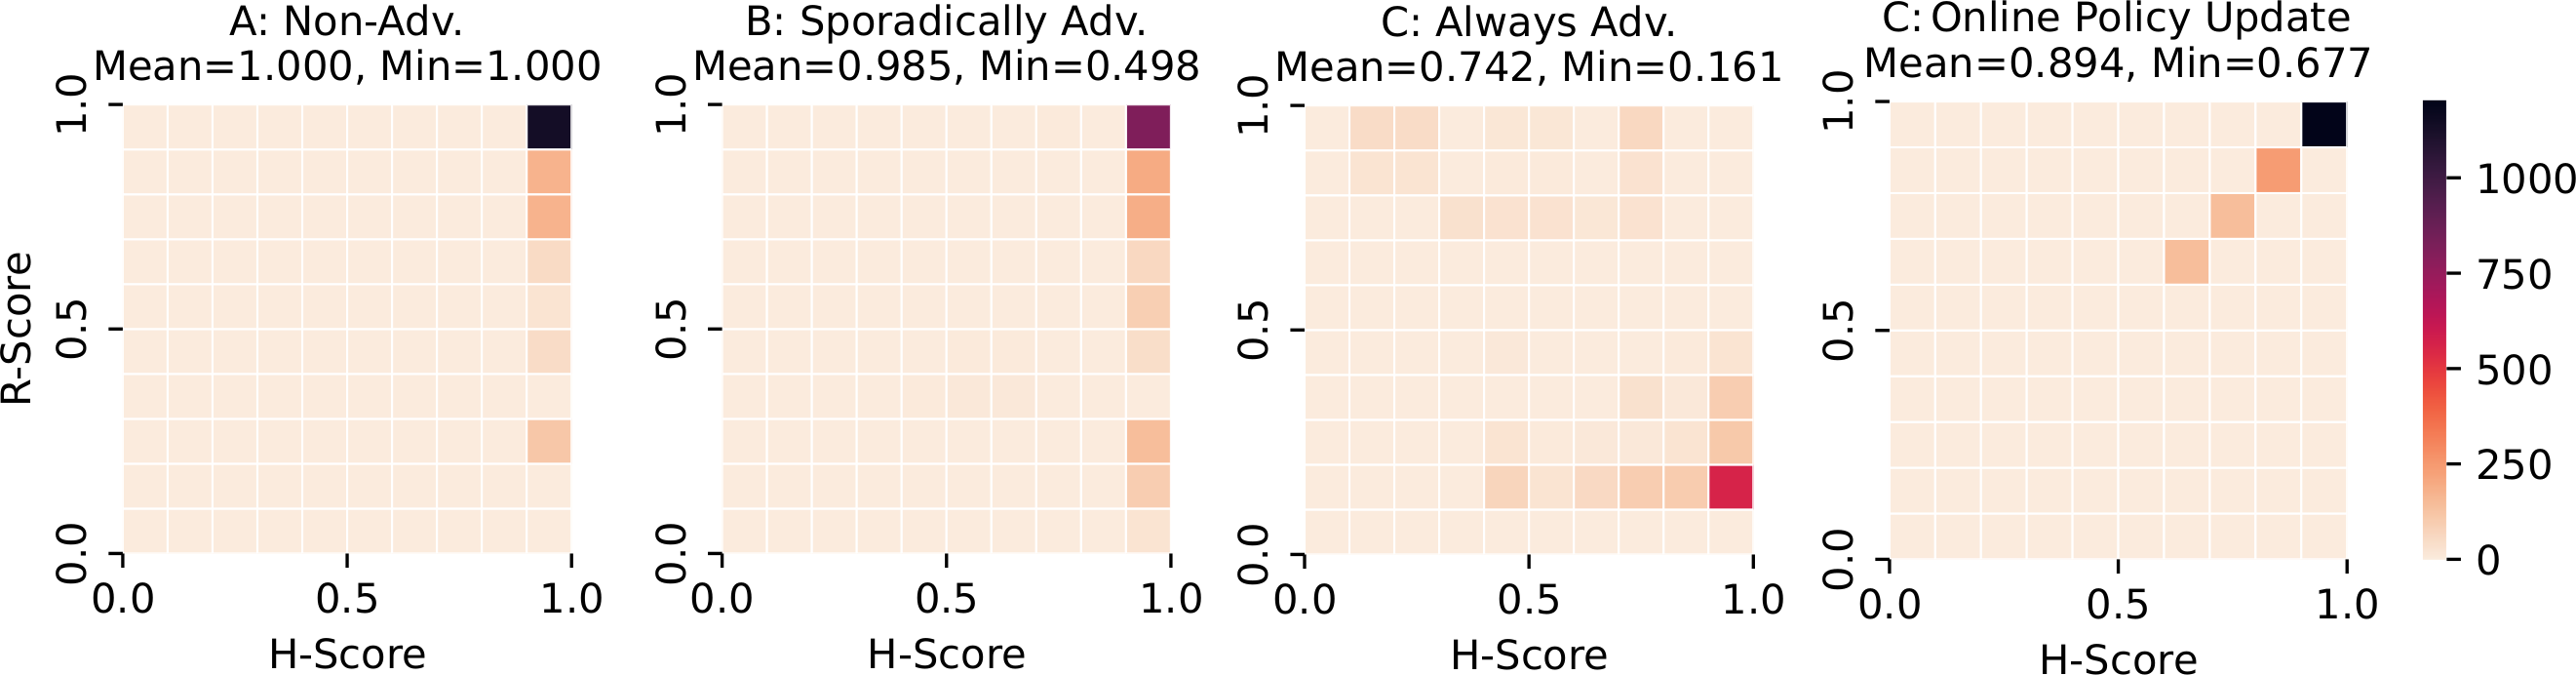
\includegraphics[width=\linewidth]{Chapter4/quant_results.png}
    \caption{
    R-scores and H-scores of the obtained executed plans after simulating the execution of the robot and the human policy generated by considering three problems and three sets of pairs of preferences/estimations. 
    The estimations in each set are (A) Never, (B) Sporadically, and (C) Always adversarial. On the right, it is shown the scores obtained using an enhanced human policy that can correct online the robot's estimation while using the set (C). \textbf{TODO: [show H mean+min and R mean+min ?]}
    }    
    \label{fig:heatmaps}
\end{figure}

For the simulations, we first generated three problems of the BlocksWorld domain with different initial states and shared tasks, and we produced for each their corresponding search graph. 
After, we generated numerous pairs of human preferences and associated robot estimation, all those pairs are categorized in three distinct sets.

In Set~A, the estimations are mostly correct and close to the human preferences (case \textit{(1)} in figure~\ref{fig:corr}). Set~B includes incorrect estimations (case \textit{(2)} in figure~\ref{fig:corr}). And Set~C contains only adversarial estimations (cases \textit{(3)} and \textit{(4)} in figure~\ref{fig:corr}).
Then, for each preference-estimation pair and each problem we generated the associated human and robot policies. Their execution was simulated symbolically using an execution automaton directly shaped upon the presented Model of Execution, and the obtained executed trace were retrieved.
The R-score and H-score of every obtained executed trace are shown as heatmaps for each distinct set of pairs in Figure~\ref{fig:heatmaps}. This will help us to highlight the benefits of using such execution scheme.

In Set~A, the estimation of the robot is close to the real human preferences and is never adversarial. So, the robot policies (maximizing the R-score) should naturally lead to high H-scores, and this is what we observed.
Some plans had an R-score lower than $1.0$ showing that the estimation was not perfect. Yet, the compliance to the human actions and the non-adversarial choices of the robot allow to always satisfy the maximal H-score of $1.0$, and thus, to always satisfy the human preferences. 
With Set~B, the incorrect estimations induced some detrimental robot choices, preventing the human from always reaching a score of $1.0$. This is depicted by the minimal H-score of $0.498$ obtained. Nonetheless, the average H-score of $0.985$ indicates that the human preferences were overall largely met.
Set~C captures the worst possible estimations inducing the robot to always make adversarial choices. This is depicted by the lower average H-score ($0.742$) and the very low minimal H-score obtained ($0.161$). 
Yet, we can notice that the average H-score is still high and that the R-score drops significantly. A low R-score means that the robot wasn't able to follow its policy correctly. Indeed, thanks to our model of execution, the robot comply to the human online decisions and purposely deviate from its ``optimal'' policy to let the human follow their own optimal policy. Eventually, the relatively high H-score obtained shows that the compliance is effective and compensates significantly (of course not totally) for a very poor estimation of human preferences. 

Additionally, we can reasonably complement the human policy, which is so far only based on preferences, with a \textit{rule}. Whenever the robot performs an action that degrades significantly the best reachable H-Score, then the human reacts by correcting online the robot estimation.
The rightmost sub-figure in Figure~\ref{fig:heatmaps} shows the new scores obtained using the Set~C and the complemented human policy. 
We notice that correcting online the estimation avoids very low human scores (minimum of $0.677$), and increases significantly the average H-score as compared with the original Set~C results (from $0.742$ to $0.894$). Hence, making the robot compliant with online preferences is very effective in improving the quality of the joint plan executed.

\textbf{TODO: [Comparison with baseline ??? ... this lack was criticized... A simple baseline with Robot first? Should show that on correct is fine but then H-score is highly degraded... Should be a mirror case of our results However, must replicate results and create more... currently unclear if can replicate.]}

Overall, we can see that the compliant robot behavior regarding both online human actions and preferences benefits the collaboration thanks to the high human scores obtained.

Consider some counter-cases from social robotics (or HA collaborative planning). Assume a robot not giving the initiative to humans always executing the best action it found. 
It is less acceptable and restricting for humans this way, even if the robot computed its best action by taking into account some social rules and estimated preferences. 
Unlike here, humans would appear compliant with the robots. 
In those cases, as it is evident from our simulation results in adversarial setups, the robot strongly impacts the solution H-score. Thus wrong robot choices can significantly degrade the human scores. In some sense, being compliant and adjusting to online preferences can be seen as some social factor that robots should maximize, and our framework helps achieve that.

\section{Performances}


In this section, we discuss the computational performances of our approach and provide some empirical measurements. 

Our approach is based on exploring every decision the human is likely to make and every possible robot concurrent and compliant actions to those decisions. 
This offline search produces a directed acyclic graph (DAG) which captures all possible courses of action. Then, from this graph, we can easily extract online the optimal robot policy to adapt to and to satisfy the human preferences. However, this exhaustive approach does not scale since the more complex and long the task is, the more possible coodinations and courses of actions exist, and the longer it takes to produce the graph. Despite this existing combinatory explosion, I would like to discuss and explain why our approach is still relevant.

Two cases can be identified. The first one is in industrial setup and the other in a household environment. Industrial tasks can be complex, constrainted, and where mistake can have heavy consequences. However, household tasks are usually simpler, shorter, and have fewer constraints and consequences. Due to the nature of industrial tasks, there is usually a known pre-defined protocol or plan to solve the task. The human is also in a working mental state, being more focused and willing to collaborate and accept robot decisions. This means that in such setups, it is more acceptable for the robot to produce a joint plan and negociate with the human to accept and follow it, without anticipating every possible human decisions which significantly reduces the complexity of the planning algorithm.
On the other hand, when considering household tasks, which is more our focus in this work, we want to preserve the human's latitude of choice as much as possible to allow them to change their mind, be distracted, or impose their choice. For this reason it is effective to run an exhaustive search and account for every possibility. 

Overall Human-Robot Collaboration scenarios never requires long plans, especilaly household taks, and are often limited to about 20 actions per agent. For such length, our exhaustive approach performs efficiently. Its takes about $0.40s$ for our approach to produce the DAG for the BlocksWorld task described in chapter~\ref{chap:6}. This graph comprises $700$ nodes and $6$ leaves, corresponding to $6839430$ different possible plans of length $19.77 \pm 1.59$ steps. With millions of plans we explore sufficient possibilities to address correctly such collaboration problem. Moreover, it takes only $0.02s$ to extract the robot's policy from the produced graph. 

\textbf{TODO: Try to add more numbers, about the task of Chapter 4 with box, and about more complex and long tasks}


\section{Discussion and Limitations}


This section discusses a few limitations of the proposed approach and possible future works to overcome them. 

First, in order to explore relevant courses of action, we assume a step-based progression toward the goal. Hence, we assume that the human and the robot must synchronize together after every action. This can work efficiently as long as we assume that all actions have roughly the same durations. However, in practice, this is never exactly the case and one agent must wait for the other at every step. Since the robot tends to be slower, the human might have to often wait for the robot during the collaboration with these assumptions. To be implemented on a real robot, this approach requires an additional execution scheme supervising the plan execution. In specific situations, this scheme could skip one synchronization and synchronize after the next step. Such a scheme could allow the human to perform more actions than the robot before synchronizing and thus promote a smooth and flexible execution.

Speaking of execution, the results presented in this chapter have only been simulated symbolically, without durative actions nor real human decisions. The next two chapters (\ref{chap:5} and \ref{chap:6}) present a user study conducted on an interactive simulator where participants collaborated with a simulated robot executing the produced policy. To do so, we created an execution scheme able to supervise the execution of the robot policy with agent synchronizations. This scheme is directly based on the model of execution presented in fig.~\ref{fig:complete_model_exec}. Thus, it relies on the steps and doesn't provide the flexible execution mentioned just above. 

Additionally, in the proposed model of execution, the robot always gives the initiative to the human. We show that this decision makes the collaboration robust to erroneous human preference estimations, and thus, is beneficial. However, it could be relevant for the robot to sometimes intelligently switch from follower to leader. Indeed, currently, even when there are no possible conflicts between agents' actions, the robot waits for the human to start acting to begin. Such synchronization isn't really necessary, so the robot could start acting directly to solve the task faster. 

Eventually, the plan evaluation is a bit limited. For now, plan selection relies on the estimated human preferences which are a list of metrics to maximize or minimize in the priority order given by the list. This means that there is no balance between the metrics so, depending on the ordering, a plan of length $N$ where the robot is never intrusive and always compliant could be rejected against a plan of length $N-1$ where the robot is intrusive twice and never compliant. 
Yet, in our examples, we tend to explore numerous very similar possible plans. Thus, there are always several possible plans with a same top-priority metric value, e.g. plan length, and the ordering will help select the best plan satisfying at best the other listed metrics.   

\section{Conclusion}

We addressed the complex challenge of concurrent task planning for a shared goal in the context of human-robot collaboration, acknowledging the inherent need for autonomy in humans' choices of `what' and `how' aspects during task execution. 

Based on studies about joint action, we formulate an execution model, and we present a new human-aware task planner designed to accommodate the uncontrollability factor inherent in human agents while employing this execution model leveraging social signals to facilitate the exploration of human-robot joint actions and a smooth execution. 
We also propose a plan evaluation and selection based on estimations of the human inner preferences.
As a result, the planner produces the behavioral policy for a robot that complies with online human decisions and their (online) provided estimated preferences, 
ensuring it solves the task, satisfies at best the estimated human preferences, and allows smooth and sound execution of concurrent joint action.

We provide a detailed account of the novel planning process and joint action model. We demonstrated its effectiveness through symbolically simulated BlocksWorld scenarios and how our model makes the robot robust to erroneous preference estimations.

Additionally, as mentioned in the previous section, we implemented an interactive simulator in which a real human can collaborate with a simulated robot running the generated policies. We used this simulator to conduct a user study to validate our approach with real humans. This simulator and study are described in the next two chapters.  

% \ifdefined\included
\else
\setcounter{chapter}{4} 
\dominitoc
\faketableofcontents
\fi

\chapter{User Study to evaluate an integrated plan and execution scheme in simulation}
\chaptermark{User Study to evaluate an integrated plan and execution scheme in simulation}
\label{chap:5}
\minitoc

\section{Introduction}

why simulation: HRI rebuttal: we rely on a reactive execution, real life robot are slow and not very reactive thus may bias our results

Thus, we developed an interactive simulator running robot policies generated as explained the Chapter~\ref{chap:4}. Then, we conducted a user study using this simulator to evaluate our approach.
First, the simulator is described (planning and exec part). Then, the Procedure of the Study is presented. Eventually, the obtained results are presented and then discussed.

\section{Related work}
of plan+execution, simulator

\section{Interactive Simulator}
planning is same

execution is based on model of execution and mock components

human collaborates in real time with robot in blockwords task

describe simulator, mouse, robot and human capabilities, goal shown, prompt

Synchronization, internal communication through simulated visual signal, explicit reaction time, ID phase currently always successful a success rate can be given. 


***********

In this section we provide a few functional and technical details about the developed interactive simulator used for the User Study, its overall structure is shown on fig~\ref{fig:iteractive_simulator}.

\begin{figure}
    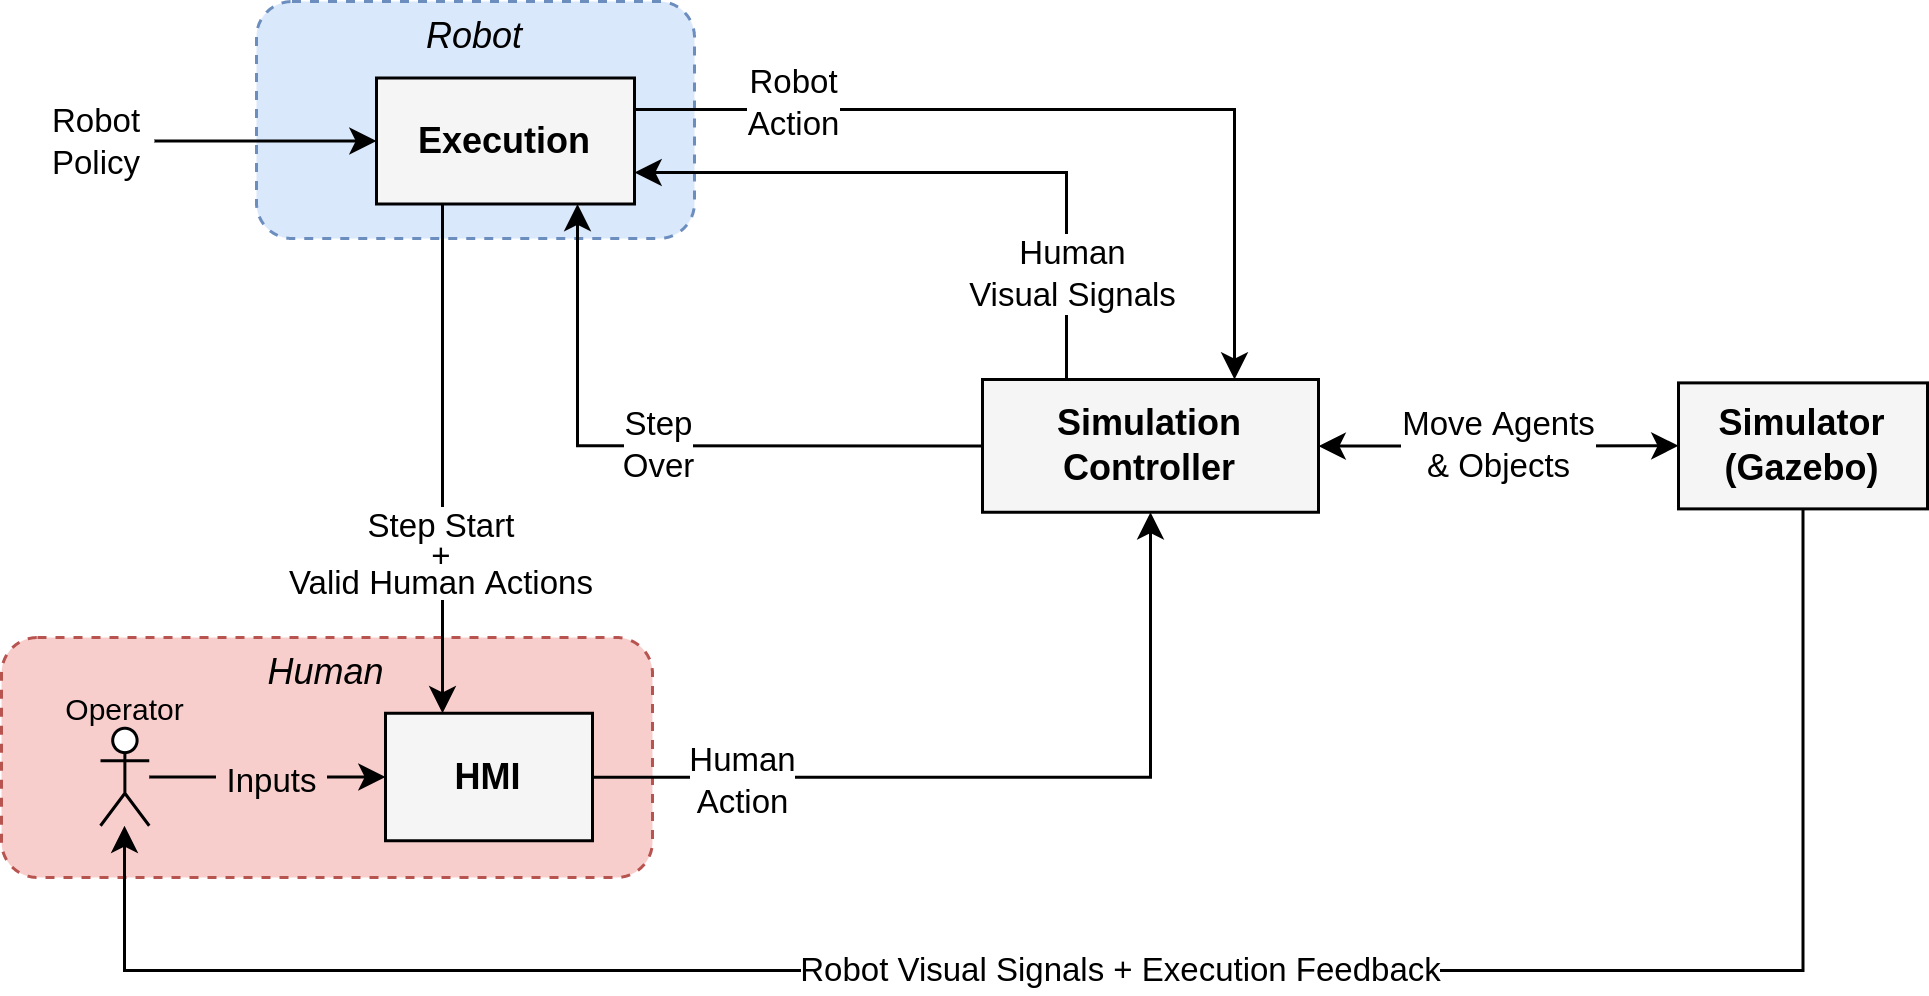
\includegraphics[width=\textwidth]{images/Chapter5/simulator.png}
    \caption{Interactive Simulator Overview}
    \label{fig:iteractive_simulator}
\end{figure}

First, it is using Gazebo to simulate the scene (table, cubes, agents). 
The robot is a Tiago robot from PAL Robotics. We used a MoveIt controller to plan and execute arm motions. We used a publicly available component to control the gaze of the robot. The head behavior is ad hoc and designed by us.
The human agent is simulated only with its hand which is moved with a handmade dedicated controller. 
For simplicity reasons physics of objects isn't simulated, thus, each agent interact with the scene by statically attaching/detaching object respectively to the robot's gripper or the human hand.
A higher level component called the simulator controller is in charge of translating primitive actions to low level commands and calling the previously presented controllers to make the agent perform actions. Since it manages agent's action, it is also in charge of sending simulated visual signals and indicating when a step is over. Indeed, the agents synchronize themselves using simulated visual signals, and not internal signals. That is, when the human starts performing an action, a brief motion planning phase occur before effectively moving the hand, the motion visual signal is sent to the robot only at this moment. Moreover, to simulate some real perception aspect, a voluntary reaction time is introduced in the robot. Thus, the visual signal can be treated only after this reaction time is passed. A step starts when one agent starts acting (the human or the robot) and it is over when both agents are inactive. Hence, once one agent started to act the other is free to perform an action concurrently and the step will be over only when both are done. If the other agent doesn't act it will be considered as passive/inactive and the step will be over as soon as the first agent finishes.

Then we can find the respective agents' components. The robot component is an implemented version of the model of execution. Its purpose is to supervise the policy execution of the robot while running the automaton described in the model of execution. In practice, the robot starts by indicating when the step started with a sound signal. Then, it waits to receive the visual human signals for a defined amount of time. Without any visual signal the human is considered as passive. The human can either start acting (how will be described just after), which will eventually send a visual signal to the robot, or the human can make an explicit hand gesture to indicate to the robot that they will be passive (this doesn't force the human to be passive for the whole step). Note that even if the robot received the human visual signal of the human starting to act, the actual action being performed isn't yet identified, it only means that the human started to act. The robot must perform a dedicated identification process (ID Phase/Process) to identify the human action. We assume that the hand gesture that the human can make is always successfully identified instantly (without ID Process). Once either the signal received or the time-out reached, if the best robot action doesn't depend on the human decision then the robot can directly start executing this action. The robot action choice is sent to the simulator controller that will start executing the action. If the best robot action depends on the human decision then the human decision must be identified and the ID Process is run. Only after the robot can perform the best action indicated by the policy which is compliant with the identified human action. If the ID Process fails then the robot remains passive, this case is already part of the policy.
Eventually the robot waits for the step over signal from the simulator controller and run the Assessment Process. The latter identify what happened during the step (which action the human performed, even if ID wasn't necessary) and in which state we are to be ready to execute the next step and progress in the policy and toward the goal. 

The human action execution consists in the following. First, the gazebo simulator is made as the main Human-Machine Interface (HMI). Through a handmade plugin one can mouse click in the gazebo simulator window. The click position is sent on a ROS Topic and treated in a dedicated node to potentially trigger a human action. For instance, clicking on a cube starts a "picking" action with the corresponding cube as parameter, clicking on the stack area starts a "place" action, clicking on the table while holding a cube starts a "hold" action, and clicking on the hand make an explicit hand gesture to signal the robot the human desire to be passive. After clicking the hand once, the participant can click another time to indicate the robot full passivity until further notice. The robot will consider the human as unavailable or even not present and will not wait for them. 
For this to be possible we did the following. First, another gazebo plugin has been written to lock the GUI camera as a First Person View and avoid the participant to accidentally move the camera.
Then, at every step, the robot component sends to the component receiving the coordinates of the click the currently valid human actions that the participant can perform. Thus, the participant cannot try to place a cube without holding it. Eventually, each human action is mapped to a clickable zone on the gazebo window. Hence, when the click coordinates are received, we check if it is inside one of the designed zone and is the action associated to the zone is currently valid. If so, then the action decision is sent to the simulator controller to be executed. 
For clarification purpose, when clicking on a cube the robot doesn't immediately know that the human is picking a cube. First, it will know that the human started to act only after receiving the visual signal (after the defined reaction time). And the robot must perform an additional perception phase (ID Process) to identify which action the human performed. 

Additionally, the stacking goal pattern is shown inside the simulator and a small prompt overlay is present to simulate a potential screen with which the robot can communicate its intention to the human during the collaboration. 

Thanks to all these processes, the participant is able to intuitively perform actions using mouse control and can collaborate with the robot to solve the task.

An integrated tutorial has been made to familiarize the participant with the mouse control and the relevant concepts used in the collaboration (notion of step, able to be passive). 



\section{Study protocol}

objective, participants, material, experiment design, procedure, measures

This section describes the objectives and protocol of this study.  

\begin{figure}
    \centering
    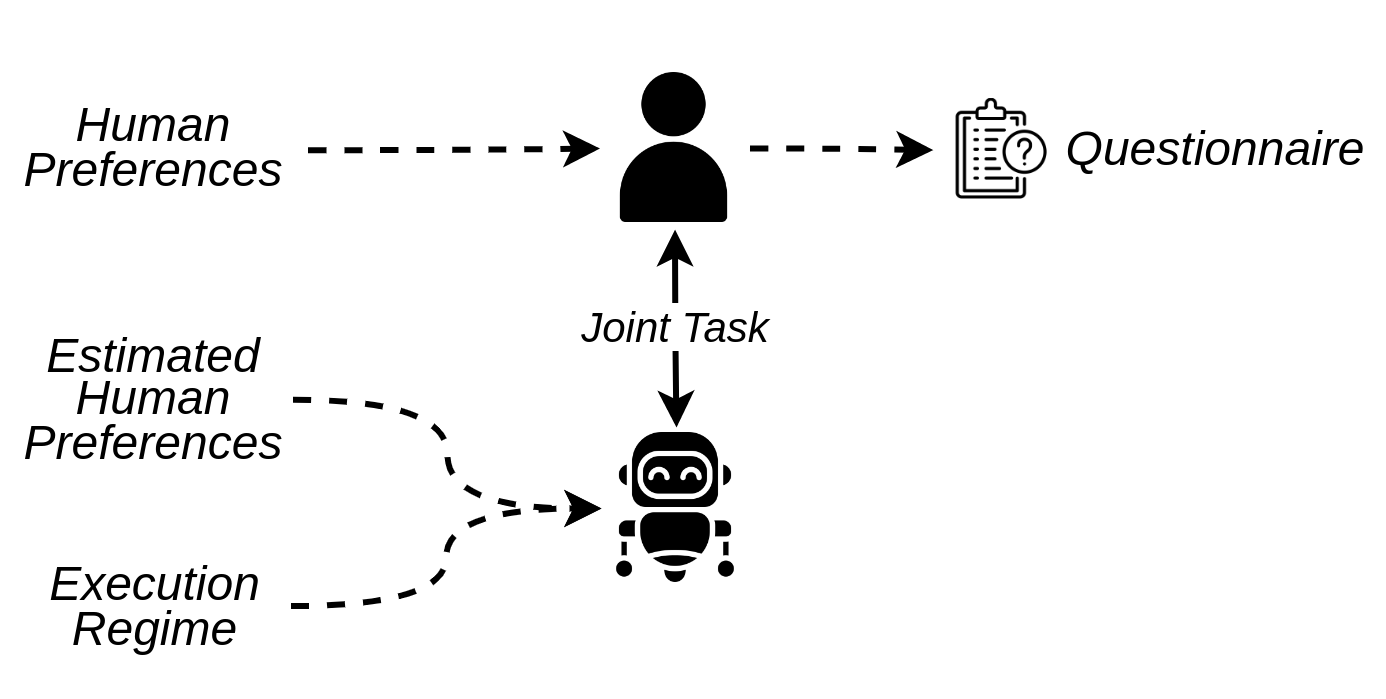
\includegraphics[width=0.8\textwidth]{images/Chapter5/UserStudyProcedure.png}
    \caption{User Study Protocol. Each participant goes through 6 scenarios and answer 6 questionnaires to evaluate each different robot behavior}
    \label{fig:user_study_protocol}
\end{figure}




Through this study we want to demonstrate the benefits of using the model of execution described in the previous chapter~\ref{chap:4} in a collaborative context. We believe this model of execution is pertinent to be taken into account when executing and supervising a robot's plan. For the same reasons we based the policy generation of this model and aim to justify our choice and validate our approach.

In this study, each participant is made to collaborate six times with a simulated robot to achieve a shared task, each time is referred to as a scenario. The robot exhibits a different behavior in each scenario. After each scenario, the participant evaluate the robot's behavior through the PeRDITA questionnaire \cite{devin_evaluating_2018}.

Beforehand, every participant answers a few general/demographic questions and is familiarized with the simulator functionalities through an integrated tutorial. Only then they start the six consecutive collaborative scenarios, answering every time a questionnaire to describe the interaction. Eventually, every participant is asked to share their general feelings and impressions about the overall interaction with the simulated robot, and they are asked to tell which scenario they preferred the most and the least.

\begin{figure}
    \centering
    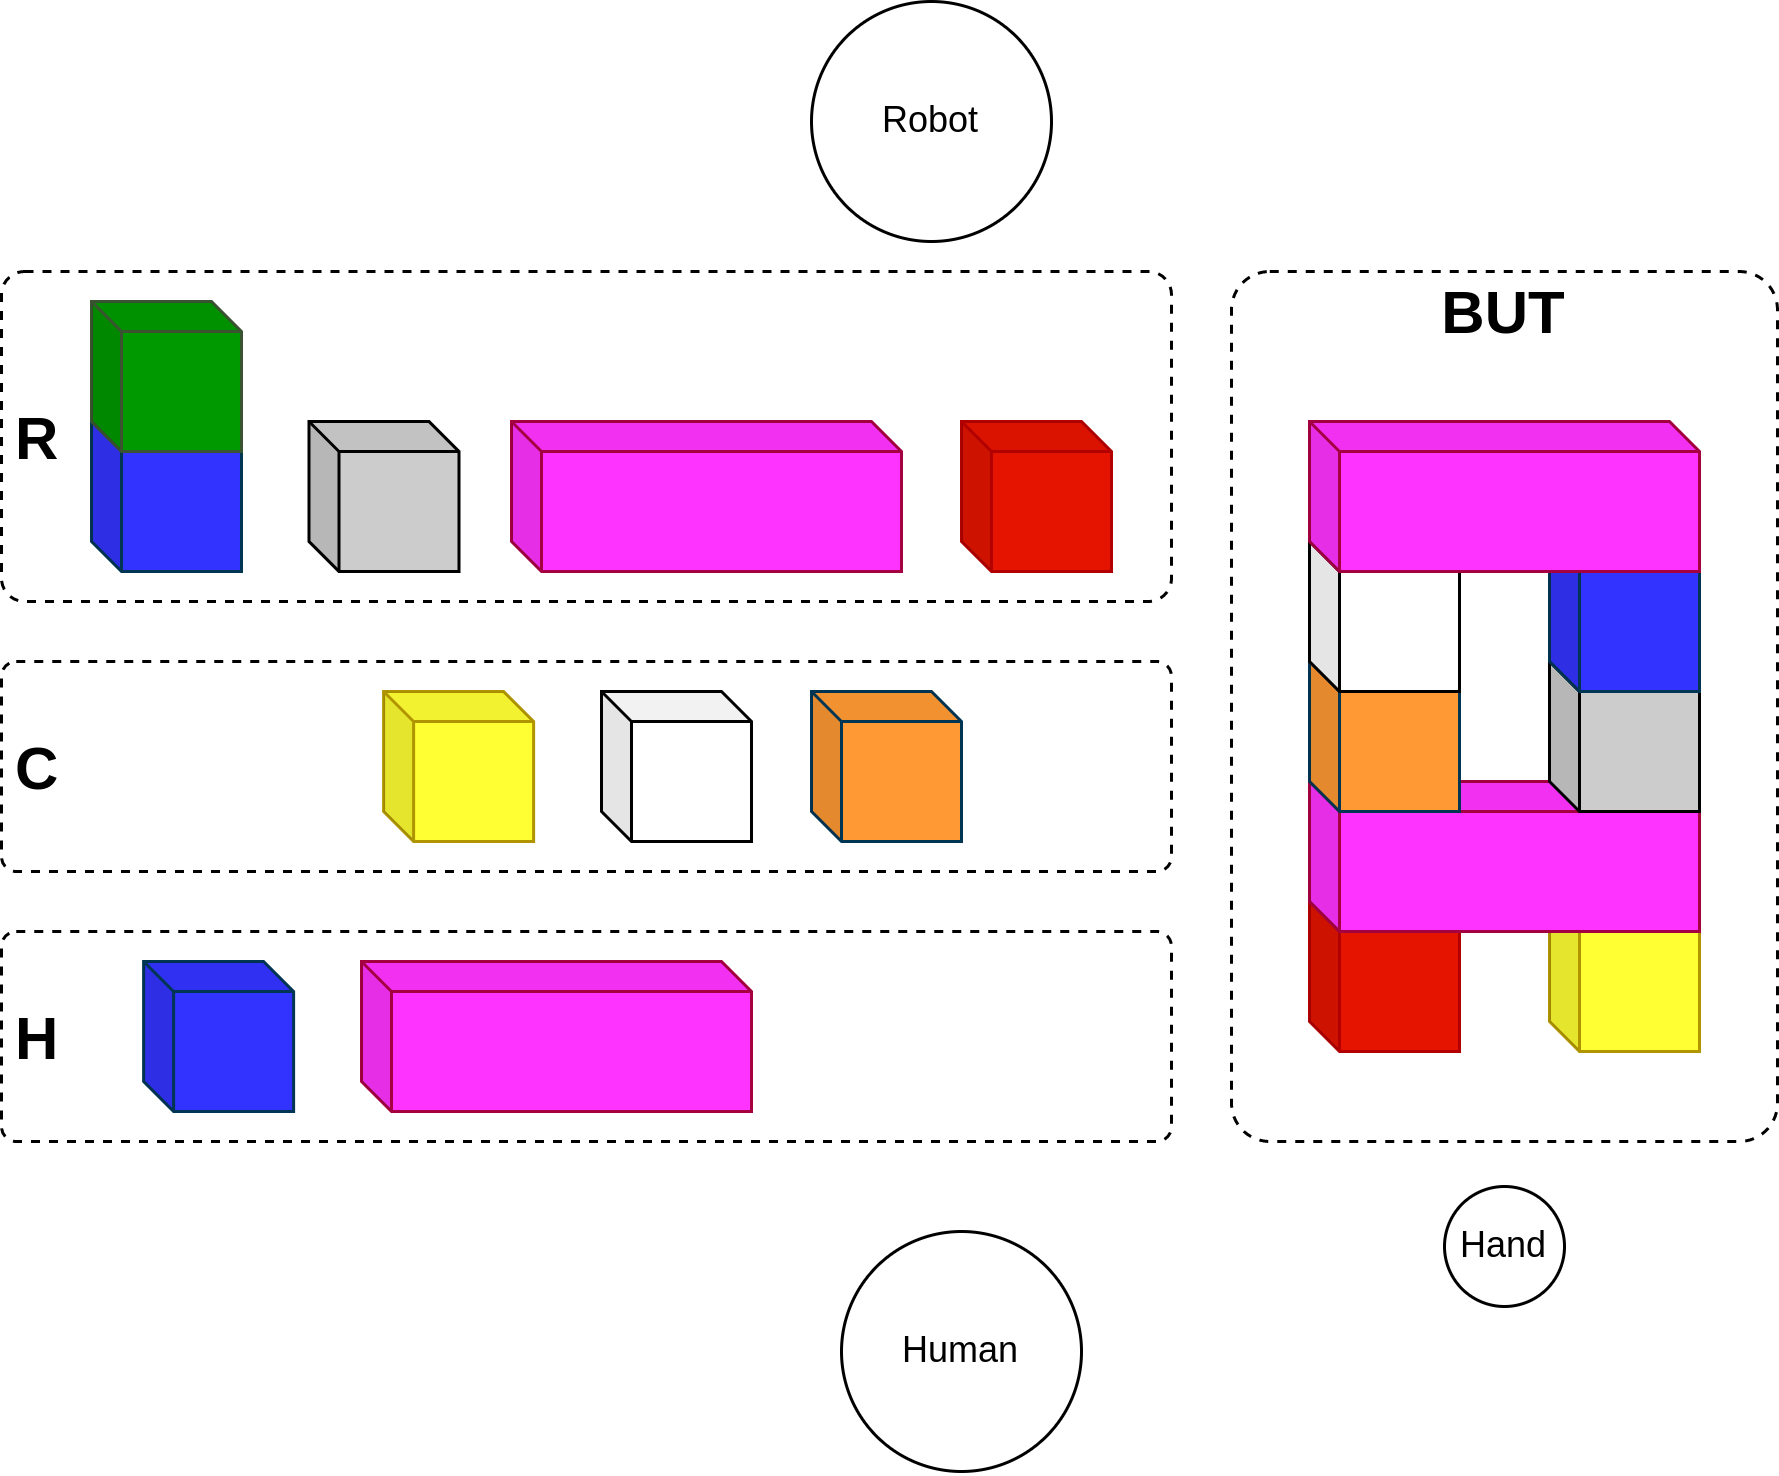
\includegraphics[width=0.8\linewidth]{images/Chapter5/task_description_study.png}
    \caption{Description of the shared task to achieve in the study.}
    \label{fig:task_description_study}
\end{figure}

We now provide details about the task, the scenarios and how the different robot behavior are generated. 
The shared goal, which is stacking the cubes to match the given pattern, remains the same in all scenarios. The cube disposition on the table also doesn't change either. The task description is depicted in fig~\ref{fig:task_description_study}. 

To progress in the task, the agents can perform three different primitive actions which are the following: \textit{pick} a cube, \textit{place} a cube in the stack, or, \textit{drop} a cube back on the table.
These actions have a few preconditions, more or less intuitive, that are communicated and experienced by the participant during the integrated tutorial.
First, one can \textit{place} a cube if they hold the cube, and if the targeted location is free and supported. That is, the cubes directly below the targeted location must be placed before being able to place a cube in the targeted location.
Secondly, one can only \textit{pick} a cube from their respective reachable zones of the table, i.e., Human and Center zones for the human, and Robot and Center zones for the robot. Also, one can only pick a cube if it can be placed immediately. Thus, one cannot pick a cube ``in advance'' and has to wait to its placement condition to be true before picking it up. For instance, both pick bars can only be picked up after the yellow and red cubes have been placed. This rule helps to create interaction conflicts serving the purpose of this study. Moreover, although the participants find this not intuitive they get used to it really fast and this feeling seems to be significantly reduced along the experiment.
Third, one can \textit{drop} a cube back on the table only if they hold it and if it cannot be placed.

For each scenario the participant is given instructions regarding how to solve the task. The participants are asked to consider these instructions as their own choice and preferences regarding the task resolution, and thus, to act accordingly while collaborating. The instructions at each scenario are one of the two following.
On the first hand, the participant shall act in a way to finish the task as soon as possible. Here, it consists in trying to perform as many actions in parallel as possible to progress faster. These preferences are latter referred to as Task End Early (TEE).
On the other hand, the participant shall act in a way to be freed as soon as possible. That is, they should finish their mandatory part of the task as soon as possible, so they could leave and let the robot finish alone. Here it consists in placing the pink bar from the Human zone as soon as possible. These preferences are latter referred to as Human Free Early (HFE).
On its side, the robot doesn't directly have access to these instructions/preferences, they are only estimated. Hence, for each scenario, the robot is given a more or less accurate estimation of the human preferences that are communicated to the participant. Note that the participants aren't aware that the robot has an estimation of their preferences, neither that this estimation can be inaccurate.
This way, we created three scenarios with different pairs of human preferences and associated estimation. In the first pair, the human shall finish the task early and the robot has a correct estimation, i.e., the robot's policy is helping the human to finish the collaborative task early. In the second pair, the human preferences remain the same, but the robot estimation is incorrect. The robot is trying, mistakenly, to minimize the human effort. As a consequence, the robot tends to pick cubes that the human could pick, preventing the human from acting and making the task completion longer. In the third pair, the human shall free themselves early, but the robot estimation is again erroneous. The robot will try to finish the task early while its priority is to place the first pink bar, which is conflicting with the given human preferences.

Additionally, in each scenario, the robot follow one of the two following execution regimes:
\begin{itemize}
    \item \textbf{Robot-First (RF)}: the robot always initiates actions first, and the participant take action afterwards.
    \item \textbf{Human-First (HF)}: the robot always lets the participant take the initiative, and then acts.
\end{itemize}
The \textit{Human-First} execution regime corresponds to the Model of Execution described in the previous chapter. At each step, the robot waits for the human's decision and will execute the best action that complies with it. The human always start acting first and the robot follows. On the other hand, the \textit{Robot-First} regime corresponds to a naive and straightforward policy execution where, at each step, the robot directly starts executing the overall best robot action given by the policy. The robot always starts acting forcing the human to comply. The \textit{Robot-First} regime serves as a baseline to evaluate the proposed \textit{Human-First} regime, described by our Model of Execution and used in the policy generation.
Eventually, we associate each of the three previous pairs of preferences and estimation with one of the two different execution regime. As a result, we obtain six different scenarios with six different robot behaviors named in table~\ref{tab:scenario_names}.

\begin{table}
    \caption{Name of the six scenarios. 
    Columns represent the preferences/estimation pairs and the rows correspond to the execution regimes.}
    % \vspace{-15pt}
    \begin{center}
    \begin{tabular}{c|c|c|c|}
        \cline{2-4}
        & TEE: correct  & TEE: incorrect    & HFE: incorrect\\
        \hline
        \multicolumn{1}{|c|}{Human-First}     & S1            & S2                & S3\\
        \hline
        \multicolumn{1}{|c|}{Robot-First}     & S4            & S5                & S6\\
        \hline
    \end{tabular}
    \end{center}
    \label{tab:scenario_names}
\end{table}

Note that our goal is to evaluate and compare the different robot behaviors. However, at the beginning, the participants don't have any references to compare with which can influence their answers in the very first scenarios. One solution is to ask the participants to answer all six questionnaires at the end, after being familiar with the six scenarios. We consider that this option demands a too heavy mental workload to recall accurately each specific scenario, and may bias the answers. As a consequence, we decided to ask the participants to answer the questionnaire after each scenario as a draft. Along the experiment, they can rectify their answers to match more accurately their feelings. At the end, using the drafts, they share their final answers for each scenario. We believe this process allow to more accurately gather the feelings of the participants. Moreover, the ordering in which the participants encounter the scenarios is uniformly randomized to prevent any order effect. 

\textbf{TODO: Give more details about the PeRDITA questionnaire (questions, goal, etc..)}

On top of the answered questionnaires, for each scenario, the interactive simulator produces logs from which we extract several metrics and an overall timeline of the execution. The timeline depicts the activities and actions of each agent along the task progression. The subjective measures done through the questionnaire are complemented with the objective metrics extracted such as the duration to complete the task, the number of human action, the total duration of human inactivity, and more. 



\section{Study results}

In this section, we share the main results obtained through the answered questionnaires and the metrics extracted from the logs.



\subsection{From timeline}
\textbf{TODO: For now with only 9 participants, it is hard to extract any relevant result from the logs. The timelines vary considerably. So far, we can say that S2 seems faster than S1. And aberrant result can be found in certain scenarios. However, we also extract the ratio of optimal human action, depicting if the participant followed optimally or not the given instructions. This metric helps to justify this aberrant results since the participant behaved significantly differently than the others.}

\subsection{From questionnaires}

Some questions have large standard deviation, such as about the perceived ``Intelligence'', but often only on specific scenarios.

The ``Reactive'' answers are overall the same, whatever execution regime and scenario. 
Overall, based on an ANalysis Of the VAriance with repeated measures (ANOVA), all other answers than ``Reactive'' vary significantly. Post tests show that the main differences come from the scenarios S4 and S6. Those two scenarios correspond to ones where the robot has an incorrect estimation of the human preferences and is following the \textit{Robot-First} execution regime. This indicates that all HF behaviors are perceived similarly despite the erroneous estimation of the robot. It also indicates that the RF scenario with correct estimation is positively perceived, but an erroneous estimation has significant impact on the answers when using RF.  

Except the ``Reactive'' aspect, answers about RF have larger standard deviation. Thus, participants tend to be more indecisive regarding RF than HF.

We notice very few significant differences on HF only.

\begin{figure}
    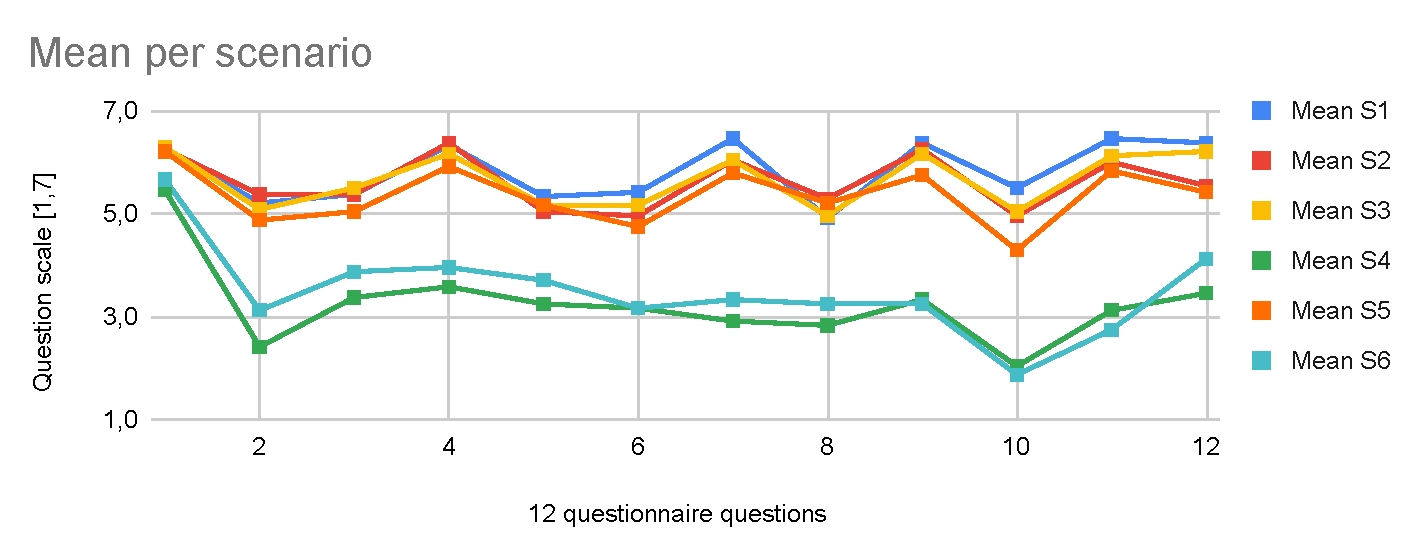
\includegraphics[width=\linewidth]{images/Chapter5/Mean per scenario.pdf}
    \caption{Mean answers per scenario}
    \label{fig:mean_per_scenario}
\end{figure}

\begin{figure}
    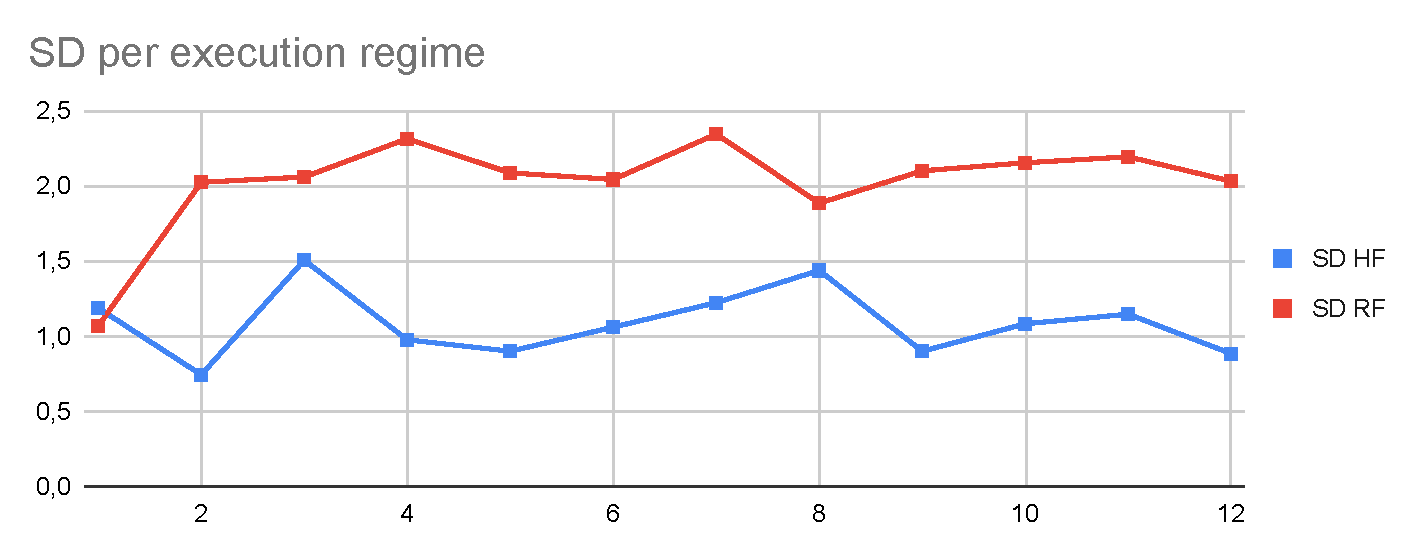
\includegraphics[width=\linewidth]{images/Chapter5/SD per execution regime.pdf}
    \caption{SD per Execution Regime}
    \label{fig:sd_per_execution_regime}
\end{figure}


\section{Discussion}



\section{Conclusion}


% \ifdefined\included
\else
\setcounter{chapter}{5} %% Numéro du chapitre précédent ;)
\dominitoc
\faketableofcontents
\fi

\chapter{Challenging Robot Navigation Systems by Simulating Intelligent Human: InHuS}
\chaptermark{Challenging Robot Navigation Systems by Simulating Intelligent Human: InHuS}
\label{chap:6}
\minitoc

\section{Introduction}
Vers simulation humain intelligent pour benchmarker planner robot (nav + tache)

An interactive simulator for user study is useful but not automated

InHuS:
ère du digital twin : 1er pas vers ça, un peu générique, fait pour nav mais pourrait aller plus loin
A mettre dans un chapitre "a part"

Objectives - Current challenges in testing ha nav

\section{Related work}

\textbf{TODO: Cite all the ones in zotero, and from paper}

\section{Description}
 
The InHuS System%
\footnote{https://github.com/AnthonyFavier/InHuS\_Social\_Navigation}
works along with a human operator, a chosen simulator, and the challenged robot controller as depicted in Fig.~\ref{fig:overview}. The system is mainly implemented using ROS. The InHuS  System is three-sided. First, the system comes with a high-level interface called Boss that helps to manage the simulated agents. Secondly, there is the main part which is the intelligent human avatar controller itself, called InHuS.
Finally, a GUI provides an interactive visualization of the data and metrics computed by InHuS during execution that can help to evaluate interactions. We present below some details for each component.

\begin{figure}[ht]
    \centering
    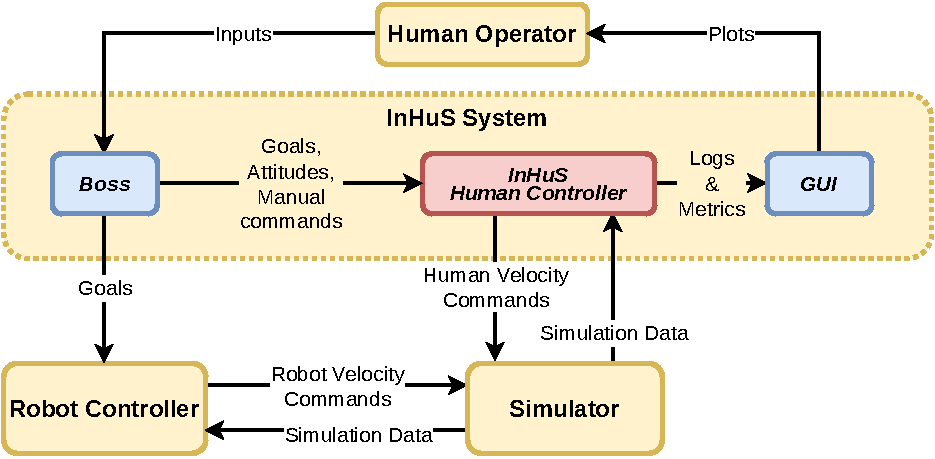
\includegraphics[width=0.7\linewidth]{images/Chapter6/Inhus.drawio.pdf}
    \caption{
    The InHuS System interacts with three external systems: the simulator, the robot controller, and a human operator. Our system is separated into three parts: the Boss high-level interface gathering inputs from the human operator, InHuS which is the actual human controller, and a GUI to plot the metrics and other data produced.
    }
    \label{fig:overview}
    \vspace{-0.8cm}
\end{figure}

\subsection{Boss}
For the human operator to easily control the simulated agents and run repeatable scenarios, we provide a simple graphical user interface component called Boss. Predefined or manually entered goals can be sent to the human, the robot, or both. Goals are by default considered as ``Pose goals'' that only require one navigation action to be achieved. However, the human agent (only) can handle ``Compound goals'' that need a specified sequence of navigation and waiting for actions to be achieved. This type of compound goal is useful to emulate more complex activities. For example, ``Make coffee'' could be described as a sequence of three actions: nav(coffeeMachine), wait(15$s$), nav(myOffice).

The Boss allows defining scenarios with start positions and goals for each agent to repeatedly generate the same situation. 
Running a scenario consists of first sending each agent to their respective starting position. Then, the corresponding goals are sent to the human and the robot.
A delay can be specified while starting the scenario to delay either the robot's or the human's goal. This is very useful to adjust the timing of a specific situation or conflict. The Boss can also put an agent in ``endless'' mode where the agent continuously gets a new goal from a given list after completing one. 

Each navigation action can specify a radius for the ``Pose goal'', within which a new ``Pose goal'' is randomly sampled. This mechanism adds randomness to the execution and diversifies the situations encountered, especially in the ``endless'' mode. Setting the radius to zero disables the randomization and selects the given goal.

All the goals, scenarios, and endless goal sequences are defined using an XML format. Hence, defining new goals or scenarios is straightforward. There is an XML goal file associated with each map/environment. Thus, it is easy to switch between environments since the corresponding goal file is automatically loaded.


\subsection{InHuS}

\begin{figure}[b]
    \centering
    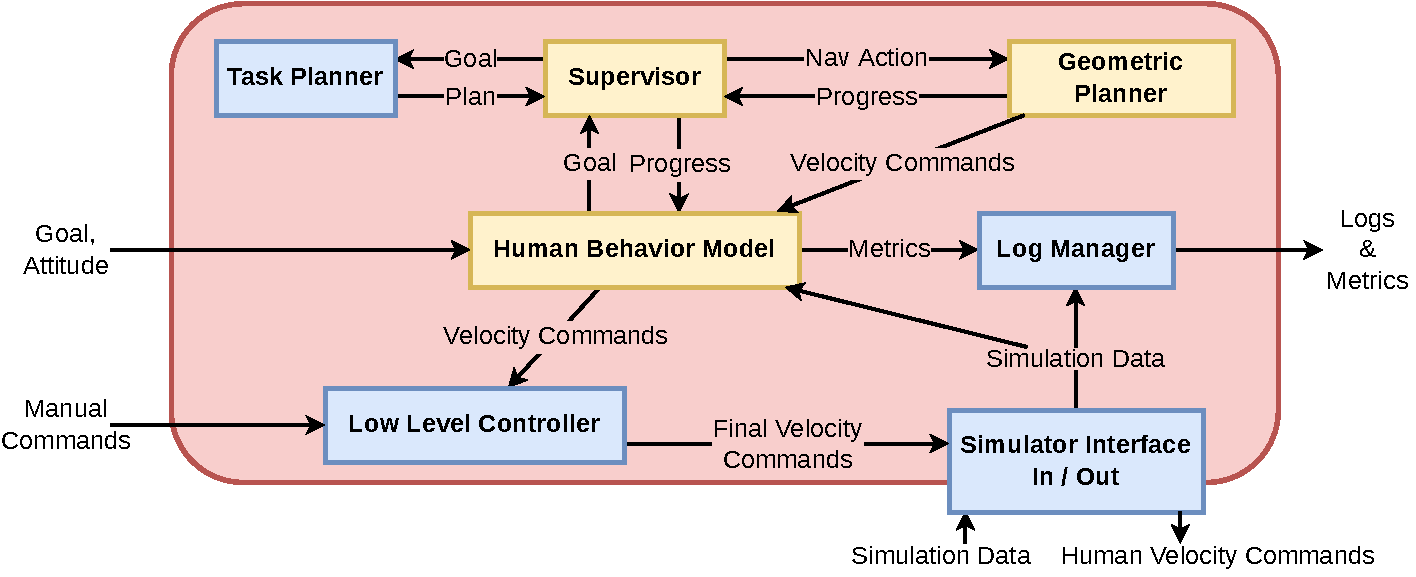
\includegraphics[height=120pt]{images/Chapter6/inhus_2.pdf}
    \caption{
    The human controller InHuS with its components and subsystems. 
    }
    \label{fig:inhus_only}
    \vspace{-1cm}
\end{figure}

The macro component InHuS is mainly in charge of controlling the avatar and generating rational behaviors. InHuS itself is made of several components as depicted in Fig.~\ref{fig:inhus_only}. However, three components, namely HumanBehaviorModel, Supervisor, and GeometricPlanner, constitute the major functional part of InHuS. We discuss each of these major components in detail.


\subsubsection{HumanBehaviorModel:}

The HumanBehaviorModel is responsible for most of the rational behavior of the agent. The first role of this component is to manage the goals. Goals can either be received from the Boss component or generated by the HumanBehaviorModel using the same XML file as the Boss. When a goal is selected, it is sent to the Supervisor for execution. 

This component is also responsible for detecting and handling navigation conflicts. Currently, the kind of navigation conflict handled by InHuS is path blockage (e.g. another agent standing in a doorway). While the human agent is navigating, a path to the goal is calculated at regular intervals using Dijkstra's algorithm, and its length is tracked to detect such conflicts. If the tracked path length increases significantly or the path ceases to exist, it could mean that another agent is blocking either the only possible way or the shortest way. When such situations are detected, the plan execution is temporarily suspended, and the agent performs an approach action to get close to the blocking location. This shows the agent's intention to move in a specific direction and might induce the blocking agent to react and clear the way.
Eventually, once the avatar is at a specified distance of the blocking location, here set to \SI{1.5}{\metre}, the agent stops its approach and actively waits for the path to be cleared.

To generate a lot of different and specific situations, we created what we call \textit{Attitudes}. They are operating modes affecting both goal decisions and reactions toward the other agents. One can activate them through the Boss to generate diversified behaviors of the agent. Some of the \textit{Attitudes} currently implemented in InHuS consist of: 1) randomly picking a new goal, like someone suddenly changing their mind, 2) harassing the robot by constantly going in front of it, like a child would do \cite{nomura2016children}, and 3) stopping close to the robot and looking at it for a few seconds before resuming its goal which emulates a curious behavior. 

The final purpose of this component is to build the perception of the human agent based on the map and information about the other agents from the simulator. We build the perception by directly accessing the simulation data rather than adding simulated sensors to the human avatar. Using this perception, we compute the visibility of the human agent and then update the human's knowledge about the robot's position and speed.

\subsubsection{Supervisor:}
The Supervisor is a central component as it coordinates different components to execute the plan and achieve the current goal. When the Supervisor receives a goal from the HumanBehaviorModel, it requests the TaskPlanner component a plan to achieve the goal. For now, the plan generation is quite simplistic. For a ``Pose goal'', a plan filled with a single navigation action is generated. For a ``Compound goal'', the sequence of navigation and waiting actions is extracted from the XML goal file and the plan is populated. Despite the simplistic plan generation, this architecture handles complex goals that require several steps to be achieved and emulate human activities.  

The execution of each action of the plan is then supervised by the Supervisor by sending requests to other components. 
When a navigation action needs to be performed, the Supervisor starts by sampling a random position if the given action radius is not zero. Then, it requests the GeometricPlanner to plan for the target position without considering other agents initially. This way, the avatar starts following the shortest path, and we initialize the conflict detection. After this, the system starts to consider the other agents, and the Supervisor periodically requests the HumanBehaviorModel component to check for potential navigation conflicts. The Supervisor can suspend and resume the plan execution at any time, which can be used to resolve the detected conflicts or to generate specific reactions like the \textit{Attitudes}.

\subsubsection{GeometricPlanner:}

The last major component is the GeometricPlanner. This motion planner component receives a target position to reach from the Supervisor and generates velocity commands to make the avatar move. This component defines how the agent moves around and adapts its velocity to the other agents in the scene. Since the system is implemented in ROS, we use the standard ROS navigation stack for the GeometricPlanner.

The planner used in InHuS is a publicly available human-aware navigation planner called CoHAN \cite{singamaneni2021human}. It is built over the ROS navigation stack and uses a local planner based on a modified version of the timed elastic band with human-aware properties. 
We benefit from the high-level decision-making of InHuS and the enhanced local navigation of CoHAN with trajectory predictions. Moreover, CoHAN is highly tunable which helps to generate different agent behaviors. 

\subsection{Logs, metrics and GUI} \label{sec:logs_metrics}

\begin{figure}[!b]
    \centering
    \includegraphics[width=0.8\linewidth]{images/Chapter6/gui_bis_bis.png}
    \caption{
    Overview of the GUI interface which is organized as follows. On the right side are shown the paths taken by the agents and colored over time. On the left side, several metrics and data produced by InHuS are plotted over time on graphs. Additional widgets help to configure the plots. 
    }
    \label{fig:gui}
\end{figure}

The InHuS system logs the execution data like the positions and speeds of the agents along with some computed metrics. All the logged data is sent to the GUI component, which generates interactive plots. These plots can help evaluate the interaction and thus the performance of the given robot controller. The snapshot of the GUI shown in Fig.~\ref{fig:gui} shows two kinds of visualizations. On the right side, there is a colored visualization of the paths taken by each agent. These paths are colored over time according to a corresponding legend that helps estimate an agent's position at a specific moment. The left side is composed of several plots showing some computed metrics over time. The first plot is about conflict detection and solving. It shows the length of the path to the goal computed when checking for conflicts. Without any conflict, the path length should decrease linearly over time. If it's not the case, the avatar has been disturbed during the navigation. This plot also shows the conflict state of the agent: Nominal (no conflict), Approach (conflict detected), Blocked (stopped and waiting). The subsequent plots show over time the speeds of each agent, their relative speed, the distance separating them, 
and a metric called time to collision (TTC). This metric estimates the time remaining before the agents collide with their current velocities. We can argue that TTC corresponds to a ``threat feeling'' since a low TTC value corresponds to a high threat of collision. Hence, social robots should be tuned to not exceed a minimum TTC value to make humans more comfortable.

\section{Main results}
able to numerically identify the HA behavior of CoHAN w/r SMB)


In this section, we show some results through a set of experiments to highlight how our system can help challenge human-aware robot navigation systems. First, we discuss the limits of reactive-only systems to strengthen the need for rational avatars. 
Then, we present how our system effectively challenges robot navigation systems and we interpret the corresponding plots.
Next, we show how the InHuS System can compare the human-aware performances of two different robot controllers.
Finally, we present additional experiments showing the diverse behaviors that can be produced using the \textit{Attitudes}, and how ``long runs'' can benefit the development of a robot controller.

\subsection{Limits of reactive-only agents}
\label{sec:pedsim_compare}
Most of the current human agent simulations used by the social navigation community rely either on the social force model or ORCA. In order to highlight the limitations of such approaches, we present results obtained with a PedSim\_ROS (or simply PedSim) agent. PedSim is a pedestrian simulator that uses the social force model. It is very efficient for generating crowds to test robot navigation. However, at the individual level, the simulated agents are purely reactive and have no decisional abilities like most pedestrian simulators. 

\begin{figure}
    \centering
    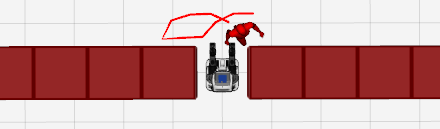
\includegraphics[width=0.4\linewidth]{images/Chapter6/pedsim_blocked.png}
    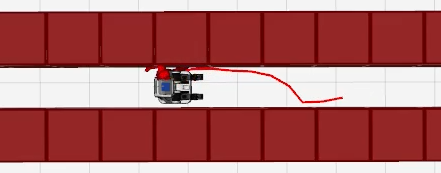
\includegraphics[width=0.4\linewidth]{images/Chapter6/pedsim_narrow_2.png}
    \caption{
    In the doorway scenario (left), the reactive-only (Pedsim) agent never stops moving while trying to go through the robot even though its path is blocked. 
    In the narrow corridor scenario (right), the agent squeezes itself between the wall and the robot colliding with both. 
    }
    \label{fig:limits_reactive}
    \vspace{-0.3cm}
\end{figure}

Consider the doorway scene shown in the left part of Fig.~\ref{fig:limits_reactive}. Both agents have to cross a narrow opening. Here, the robot is blocking the way that the human agent intends to cross. The PedSim agent approaches the robot and tries to push itself through, but it fails due to a very high value of social force. The agent never stops moving and tends to go right or left along the wall before wiggling again just in front of the robot. 
This confusing behavior can make the agent's intentions unclear to the robot planner. 
The narrow corridor scenario, shown in the right part of Fig.~\ref{fig:limits_reactive}, also exposes some limits. In this scene, there is not enough space for the agents to cross each other,  and the only solution is for one of them to back off. Here the path is blocked by the static robot. The PedSim agent slowly gets closer and closer to the robot before squeezing itself between the wall and the robot. For some reason here the social forces allowed the agent to pass, unlike the previous example. It highlights that the PedSim agent doesn't use a defined hitbox or footprint for the agent and relies only on repulsive social forces to prevent collisions. This lack of defined collision shapes makes the agent temporarily pass through the walls and other agents. As a consequence, it breaks many intricate scenarios where a rational decision should be taken and results in unrealistic situations. Despite being efficient for large spaces or crowds, based on the above observation, we can state that in intricate scenarios such approaches can lead to confusing and even unrealistic behaviors.  

\subsection{Interpretation of plots with human-aware planner}

The InHuS System is able to generate challenging situations 
and associated logs to allow further evaluation.
Here, we present one such conflict and a detailed interpretation of the corresponding plots. The plots were produced while challenging the CoHAN system in the doorway scenario.

\begin{figure}
    \centering
    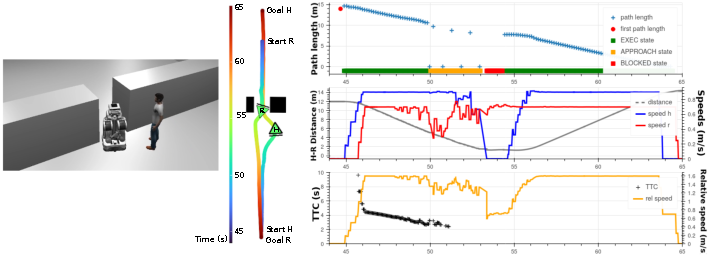
\includegraphics[width=1.0\linewidth]{images/Chapter6/test.pdf}
    
    \caption{
    A condensed view of the InHuS GUI and MORSE simulator for the doorway scenario with a robot running the CoHAN planner. Several plots depict the detection and resolution of the conflict created. 
    }
    \label{fig:cohan_passage_block}
    \vspace{-0.3cm}
\end{figure}


The robot starts closer to the opening and enters the doorway first. The execution can be analyzed with the metric plots and the time-colored paths of the agents in Fig.~\ref{fig:cohan_passage_block}. We notice that the robot's speed (red line on the second graph) goes down around \SI{50}{\second} as it is entering the doorway and creating a conflict. The conflict is detected by InHuS (zero path length = no path), and the agent switches to the approach state (green to the yellow line on the first graph).
The non-zero path length in the approach state corresponds to how the approach is performed. In order to keep moving despite the blocked path, the GeometricPlanner is requested at a defined frequency to plan without considering the robot (all non-zero path length). In between these requests, to check if the path is still blocked, the conflict detection plans while considering the robot (zero path length). When the avatar is at a predefined distance from the blocking robot around \SI{53}{\second}, it switches to the blocked state (red line) to stop and wait for the path to be cleared. Further, the time-colored paths show that the GeometricPlanner made the avatar move aside while approaching to avoid blocking the robot. As a result, the agents were no longer moving towards each other, and thus, there was no longer any collision threat (no TTC values). When there is no more collision threat, around \SI{51}{\second}, the robot's speed starts to increase again. Such behavior is a good sign of human-aware properties and might increase human comfort.

From the plots produced by our system, a lot of useful information can be extracted for improving or evaluating the social robot planner's performance like a) finding ways to decrease the blocked state time for the human, b) maintaining a particular threshold for TTC, c) slowing down near the human, or waiting for the human to cross the door without blocking.


\subsection{Quantitative comparison between two robot controllers}

Our system can be used to run similar scenarios repetitively to produce robust metric values. These values can help to evaluate the human-aware performances of a given robot controller. To show this, we present a comparison between two different robot controllers. The first one is again the CoHAN system, and the second one is the Simple Move Base (or SMB). It uses the \textit{teb\_local\_planner} and the ROS navigation stack with default parameters. We just add an additional process to consider the human agent as a static obstacle to avoid it, so it is not human-aware. Therefore, we should be able to notice a clear difference through the metrics computed by our system. For this comparison, we used three different scenarios: 1) The doorway scenario where the agents have to cross a narrow opening, 2) the corridor scenario where the agents cross each other with just enough space, and 3) the open space where they cross each other without any environmental constraints. We performed 10 repetitions of each scenario for each robot controller. For each set of 10 repetitions, we extracted the mean values of three different metrics and presented them in Table~\ref{tab:compare_robots}. The metrics are the following. First, the time to goal (TTG) is the time taken by the avatar to reach its goal. Second, the minimum distance between the robot and the human (Min HRDist). And, the minimum time to collision (TTC). Intuitively, we want the TTG to be as small as possible, the minimum HRDist to be as high as possible, and since a low TTC value represents a collision threat, we want the min TTC to be as high as possible. 

\begin{table}
\vspace{-0.2cm}
    \caption{Mean values of three InHuS metrics over 10 repetitions in three different scenarios and with two different robot controllers. Bold values indicate when the corresponding robot controller has better performance than the other.}
    \label{tab:compare_robots}
    \centering
    \begin{tabular}{|c|c|c|c|c|c|c|}
    \hline
     & \multicolumn{3}{c|}{CoHAN} & \multicolumn{3}{c|}{SMB}\\
    \cline{2-7}
    Experiment & \textit{TTG}$(s)$ & \textit{Min Dist}$(m)$&  \textit{Min TTC}$(s)$ 
    & \textit{TTG}$(s)$ & \textit{Min Dist}$(m)$ & \textit{Min TTC}$(s)$\\
    \hline
    \textit{Doorway} & 18.38 & \textbf{2.32} & \textbf{1.33} & \textbf{18.26} & 2.23 & 1.16\\
    \hline
    \textit{Corridor} & \textbf{16.34} & \textbf{2.06} & \textbf{1.03} & 17.05 & 1.59 & 0.81\\
    \hline
    \textit{Open space} & \textbf{9.55} & \textbf{2.52} & \textbf{1.61} & 11.01 & 2.34 & 1.18\\
    \hline
    \end{tabular}
\vspace{-0.3cm}  
\end{table}

At first glance, we see in Table~\ref{tab:compare_robots} that almost all CoHAN values are better than SMB values. Due to the nature of the doorway environment, the execution of the scenario is quite constrained which explains why the values are not too different between the two controllers. However, we notice anyway that, compared to SMB, the CoHAN planner tends to keep a greater distance between the agents and a greater TTC (lower threat of collision). The time to goal of CoHAN is slightly higher because the robot slows down when crossing and moving in the direction of the human. Thus, it is the price to pay in this scenario to maintain adequate TTC values.

In the corridor scenario, The SMB robot tends to wait until the last moment to move aside, which is threatening. On the other hand, the CoHAN robot proactively moves to one side of the corridor. As a consequence, it leaves more space for humans and reduces the threat of collision, which is visible in the obtained values. Also, this pro-activity has the effect of smoothing the trajectory of the avatar, which makes this last one reach its goal faster.

Finally, the open space scenario is a bit similar to the previous one. The SMB robot waits until the last moment to avoid the human, which puts the load of the avoidance maneuver on the human. As a result, 
the human has to move aside which extends the duration to reach the goal. Also, due to the same behavior, the SMB robot is on average closer to the avatar and more threatening. Since the CoHAN robot moved again aside early, its metric values are noticeably better than SMB.

In summary, the human-aware behavior of the CoHAN controller was captured through significant value differences in the computed metrics compared to a non-human-aware robot controller. This implies that our system can help evaluate and compare human-aware robot controllers.

\subsection{Generating different behaviors with Attitudes}

\begin{figure}
    \centering
    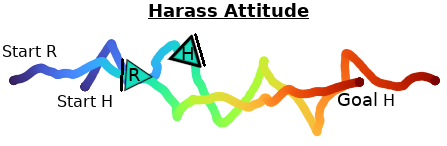
\includegraphics[width=0.45\linewidth]{images/Chapter6/harass_colored_path_bis.png}
    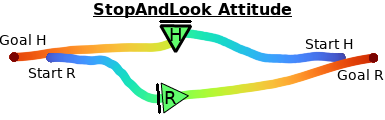
\includegraphics[width=0.45\linewidth]{images/Chapter6/stoplook_colored_path_bis.png}
    \caption{
    Behaviors obtained by activating the \textit{Harass} and \textit{StopAndLook Attitudes}. 
    With \textit{Harass}, the human is always in front of the robot.
    With \textit{StopAndLook}, when close to the robot, the human stops to look at it for a few seconds.
    }
    \label{fig:attitudes}
    \vspace{-0.3cm}
\end{figure}

By activating \textit{Attitudes}, InHuS is capable of producing more complex behaviors to diversify the conflicts and challenges imposed on the robot.
We present the time-colored paths for the execution of two \textit{Attitudes} : \textit{Harass} and \textit{StopAndLook} in Fig.~\ref{fig:attitudes}. Concerning the \textit{Harass Attitude}, by paying attention to the colors, we see that the human is always in front of the robot that continuously tries to avoid the harassing agent causing erratic movements. The robot should be able to detect such non-cooperative behavior from humans and act accordingly.
On the same figure we see the execution of the \textit{StopAndLook Attitude}. The color discontinuity behind the human marker shows how the human suspended its goal to stop and briefly stare at the robot before moving again. A robot not pro-active enough could be disturbed by the sudden stop of the human, which could be a situation of interest to handle. 


\subsection{Long run scenarios}


\begin{figure}
    \centering
    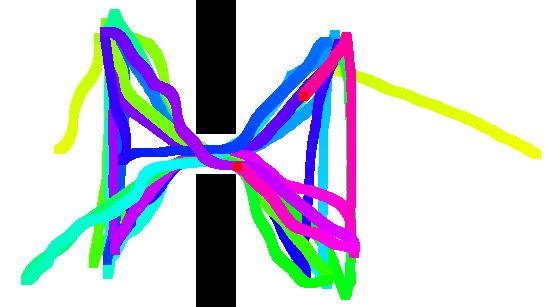
\includegraphics[height=80pt]{images/Chapter6/TDP_long_run_path.png}
    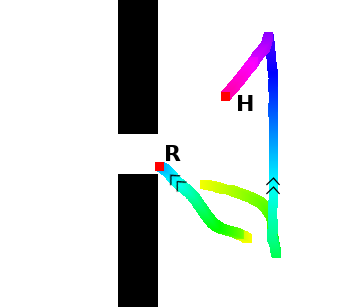
\includegraphics[height=80pt]{images/Chapter6/TDP_long_run_path_blocked_cropped_final.png}
    \caption{Execution of the long run scenario using the TDP robot planner and InHuS. We see the complete set of time-colored paths on the left. On the right, the same path is cut, around the moment when the robot got stuck in the wall. 
    }
    \label{fig:long_run_block}
    \vspace{-0.3cm}
\end{figure}

The proposed system can help test the stability and robustness of the robot planner by conducting long randomized runs. Indeed, thanks to the Boss component, possibly randomized goals can be sent autonomously to the agents. This can generate unexpected situations and conflicts that can be of interest.
Fig.~\ref{fig:long_run_block} depicts such a test conducted with InHuS and a human-aware robot planner from Kollmitz et. al. \cite{kollmitz_time_2015} here referred to as TDP. The agents were made to endlessly loop over four goal-positions (each with a \SI{1}{\metre} radius) in reverse order to create as many conflicts as possible. After 3 minutes, the robot got stuck in the wall of the doorway, indefinitely blocking the path for the human. In addition to highlighting problematic situations where the robot doesn't act as expected, long runs can expose low-level issues like unexpected crashes or memory leaks.


\section{Extension: IMHuS}

This work has been extended through the help of an intern to the IMHuS framework \cite{hauterville-2022}.

\subsection{Describe}
\subsection{results?}

\section{Discussion and Limitations}
\section{Conclusion}
% \chapter{Conclusions}
% \addstarredchapter{Conclusions} 
\markboth{Conclusions}{}

% The final remarks, lessons learnt, and future perspectives are discussed in the Conclusions chapter. The supportive work presented in Appendix A shows how an intelligent human agent is developed for the case of HAN. Further, different methodologies employed to simulate human agents for testing our HAN system are also presented. Throughout this thesis, whenever we refer to robot navigation, it is always a mobile robot with either differential or omnidirectional drive navigating on a 2D plane.

%%%%%Update this later%%%%%%%%%%%%%

In this thesis, we have explored the problem of mobile robot navigation in human environments, generally called human-aware navigation (HAN). We have presented detailed literature on how the field evolved and some existing challenges. Numerous solutions were proposed for HAN in motion planning literature by modelling humans as special obstacles. However, we believe that HAN is essentially an interaction between humans and robots. Therefore, it should satisfy the principles of HRI. In this thesis, we have put together these ideas and proposed a HAN that assesses a situation to take appropriate action. Although situation assessment and behaviour shifting have already been explored in HAN, they were mostly used on top of motion planning systems. Unlike the previous approaches, we have introduced situation assessment at the level of trajectory planning to shift between different modes of planning while the robot navigates to the goal. As this low-level mode shifting was combined with proactive planning, the robot can deal with complex situations in an efficient manner before it is too late. Proactive planning itself has some very interesting features, like quick plan adaptations and early intention shows, but there could be some very complicated situations where proactive planning may not be sufficient. The situation assessment based modality shifting is useful in such places.

We have presented three versions of our HAN system, starting with the idea of introducing modality switching inside the local trajectory planner. There were several improvements over the previous version of HATEB, and these improvements, combined with the mode switching scheme, are some of the major contributions of this thesis. Qualitative and quantitative results have shown the advantages of such an approach in various settings. We then moved on to propose a Human-Aware Navigation Stack called CoHAN with many changes to scale the system to multiple humans and to address different types of humans. CoHAN can be seen as a complete navigation stack for HAN with different costmap layers, human path prediction mechanisms, and several modes of planning that can solve most of the intricate human-robot navigation scenarios. The early intention show and the Backoff-recovery act as implicit communication mechanisms to tell the human what the robot is going to do. In the future, we plan to integrate more explicit communication through head orientation and probably voice. Various kinds of human states combined with the situation assessment can address more complicated scenarios, and to ease this, we plan to modularize the future version of CoHAN with detailed documentation. CoHAN has been tested on simulated crowds and has already shown some promising results. However, we believe that crowd navigation could be more complex, and we need more modalities and mechanisms to handle crowds efficiently. We have already presented some ideas we plan to integrate into the future version, and we expect to add more.

Apart from addressing multi-context navigation, we have also focused on one key aspect throughout the development of our HAN system, legibility. We have introduced some new human-aware constraints to make the robot's motion more legible to the human. To show the intention of the robot early, we have proposed TTC, TTCplus and Relative Velocity constraints. The Relative Velocity constraint also addresses the issue of directionality in the crossing or close-to-human navigation scenarios. We have introduced the Visibility constraint to avoid any surprises or shocks to a human when the robot overtakes the human. One more attempt to improve legibility was done through 'invisible humans’. We have introduced this concept into HAN to make sure that the robot is aware not only of the humans it is seeing but also of the environment and the places humans might emerge. We believe that this makes the system more complete and ready to face any kind of environment without behaving erratically or freezing. The `invisible humans’ concept has also made it possible to identify different places on the map through geometric reasoning and introduce different modalities of planning depending on the situation. Further, the algorithm was rigorously tested and showed satisfying performance in some very complex maps. The final version of CoHAN integrated with the `invisible humans’ has been shown to perform better and move smoothly without having any freezing robot problems. 

One of the open challenges in HAN is its evaluation, and the currently existing metrics do not do justice while the robot is navigating very dense crowds or confined spaces. As most of them are based on proxemic zones that are variable from place to place and the experiences of the person, it makes it more difficult to generalise the metrics to all cases of HAN. Therefore, we proposed some new metrics of evaluation using velocities and visibility along with distance. The velocity based metrics, $cost_{danger}$ and $cost_{passby}$, aim to measure the feeling of threat and discomfort caused to the human depending on the direction and speed of the robot's heading. Since these metrics combine distance and velocity, they can explain intricate settings better than proxemic zone violations. The first one of the vision based metrics,$cost_{visibility}$, was designed to measure how well a robot can approach a human from behind. The other metrics, $cost_{surprise}$ and $cost_{react}$, aim to measure the surprise(or shock) and risk caused when a robot appears in front of a human suddenly. The comparison between a standard navigation planner and a HAN planner showed how these metrics evaluate the `human awareness' of the system.

%%%%%%%%%%Talk about the magic numbers %%%%%%%%%%%

Human-aware navigation is not a very simple problem to address, and it taught us some valuable lessons. The developed systems are hard to validate in real-world settings. The experiments could be tedious, not easily reproducible and can be limited. Not every robot is the same. The structure of the robot matters to humans in the environment. Their behaviour towards the robot changes as the shapes and designs of the robot change. Humanoid structures are accepted better than simple mobile bases, even with the same algorithm. One of the important aspects while developing a HAN system is to have a good simulator that can generate realistic human behaviours. To this date, there is no perfect human simulator. The HAN research community has been using crowd simulators or directly testing with real humans. Crowd simulators are mostly reactive and are not realistic. On the other hand, tests with real humans are tedious and require a lot of resources and time. Although there is rapid growth in this aspect, the community is still waiting for a reliable robot simulator that can simulate rational human agents. We require more user studies to understand the intricacies of human-robot navigation. This is the right moment to invest more time into these studies, as drones and autonomous vehicles have also entered the field. The robotics community seems to have realised this, and now, there are special sessions dedicated to human-aware motion planning and human-aware navigation. The number of studies has already increased, and many researchers in motion planning are coming together to address this complicated yet interesting problem of robotics that can eventually lead to a society where humans and robots coexist.

There are already many immediate future perspectives for HAN. As autonomous vehicles have already hit the roads, it is time to make them behave socially by making them aware of humans and their intentions. An autonomous vehicle not only needs to be safe but also needs to obey certain rules and untold norms followed in society. HAN studies this problem exactly. Drones have become very affordable, and some companies are planning on using them for deliveries, while others are planning to use them as helpers in construction. All these applications require drones to navigate around humans and communicate with them. HAN in drones needs to study these in more detail and come up with better navigation systems for drones. Apart from guiding people in public places, some other applications of HAN  lie within warehouses where they need to work or deliver goods to different locations. These environments are more structured, and solving HAN in such places is much easier. HAN has been and will always be used in the sector of service robotics. Be it a robotic companion, a robotic wheelchair or robots in hospitals delivering medicines or equipment the HAN system faces dynamically changing environments where safety is one of the main concerns. A multi-context tunable navigation system could address most of these scenarios by choosing a set of parameters suitable for the setting.



% \appendix
% \chapter{Simulating Human Agents for Testing HAN}
One of the challenges during the development of a HAN system is to test the system before its final deployment and real-world runs. Robotic simulators are of great use during this period as we can test the system under various conditions and in several environments. Unlike the classical setting, testing HAN requires the simulation of humans, which is still research under development. Until recently, the HAN community used the crowd simulators like Pedsim or MengeROS~\cite{aroor2017mengeros} to simulate humans in semi-crowded or crowded scenarios. However, the motion generated by these simulators uses reactive schemes like \acrshort{sfm} or \acrshort{orca}, which are good for generating crowds but lack intelligence at the level of an individual human. Recent simulators like SEAN~\cite{tsoi2020sean, tsoi2022sean} and SocNavBench~\cite{biswas2022socnavbench} tried to generate somewhat intelligent behaviours using new approaches and real-world data. However, these human agents are either not reactive (as they replay real-world trajectories without considering the robot) or use schemes similar to \acrshort{orca}. Although they have better human agents and environments for testing HAN, they still lack intelligent agents that can be used to test intricate scenarios in spaces like offices, labs or homes. Hence, we have used different ways to control the human(s) while testing the HAN proposed in this thesis. These ways include manual control using a joystick, a simple human controller that follows the generated trajectories, and finally, an intelligent human with rational decision-making capabilities.      

\section{Planning and Control for Human Agents}
In this section, we talk about the simple modes and planners employed to control the human avatar in the robot simulator. A human is assumed to be a robot with special requirements.

\subsection{Manual Control}
One of the simplest ways to control a human is to move the human manually using a keyboard or joystick. This is efficient in testing some very complicated scenarios involving intelligent decisions. Since a real human is already controlling the human avatar in the simulator, all the decision-making process is handled by the human operator. To integrate such human avatar into our system, we used the \textbf{\textit{joy}}\footnote{\url{http://wiki.ros.org/joy}} \acrshort{ros} package and then mapped the inputs of the joystick to the avatar's velocity with a cap at \SI[per-mode=symbol]{2}{\metre\per\second}.

Manual control is good for testing some interesting and particular cases, but it becomes tiresome to run several scenarios to benchmark or quantify the results. Moreover, the simulation runs cannot be completely automated as the human operator is always involved in the loop. So, the next solution was to plan and control the human, like the robot. It is different from collision avoidance algorithms as the human has a global path to trace and a separate local planner to move the human. 

\subsection{Planning based Control}
To automate and replicate the tasks easily, we have developed a simple \textbf{\textit{humans navigation}}\footnote{\url{https://github.com/sphanit/humans_nav}} package using the \textbf{\textit{global planner}}\footnote{\url{http://wiki.ros.org/global_planner}} in \acrshort{ros} and a simple controller. The developed system has two modes of operation:
\begin{enumerate}
    \item \textit{Trajectory following}: In this mode, the human follows the trajectory that is provided externally through a \acrshort{ros} topic. We used this mode to test the ideal situations where the human follows the trajectory planned by \acrshort{cohan}.
    \item \textit{Goal-based Control}: This mode is more autonomous as we only provide a goal via a \acrshort{ros} topic, and the system plans and moves the human to the goal. The planning module updates the plan as the human moves, and the simple controller traces the path. This mode was used to run multiple tests to check how well the robot adapts to the human.
\end{enumerate}
Both these modes can control more than one human simultaneously. The \textit{Trajectory Following} mode used the trajectories planned by \acrshort{cohan} to move the humans. The trajectory provided the desired velocities, which were sent directly to the human controller. However, in the \textit{Goal-based Control} mode, the velocities were calculated based on the current position and planned paths of the humans. To accept multiple goals and plan for all the humans together, a \textbf{\textit{multi-goal planner}} was developed, and it is used internally by the \textbf{\textit{humans navigation}} package to get plans based on the provided goals.

Even though this kind of system solves the issues of automation and is less tiresome to the developer, the human agent is still not intelligent and simply follows the given trajectory. Although the trajectory provided by \acrshort{cohan} takes care of many human-robot social constraints, this ideal behaviour may not be expected from humans. In the second mode of control, the human agent might have better behaviour, but the agent is still not intelligent and somewhat reactive, like in collision avoidance schemes. 

\section{InHuS}
InHuS\footnote{\url{https://github.com/AnthonyFavier/InHuS_Social_Navigation}}~\cite{favier2022_hri} stands for \textbf{I}ntelligent \textbf{Hu}man \textbf{S}imulator, and it was developed to specifically simulate a human agent that is rational and persistent about its goal, unlike the reactive schemes. 
\begin{figure}[!hb]
    \centering
    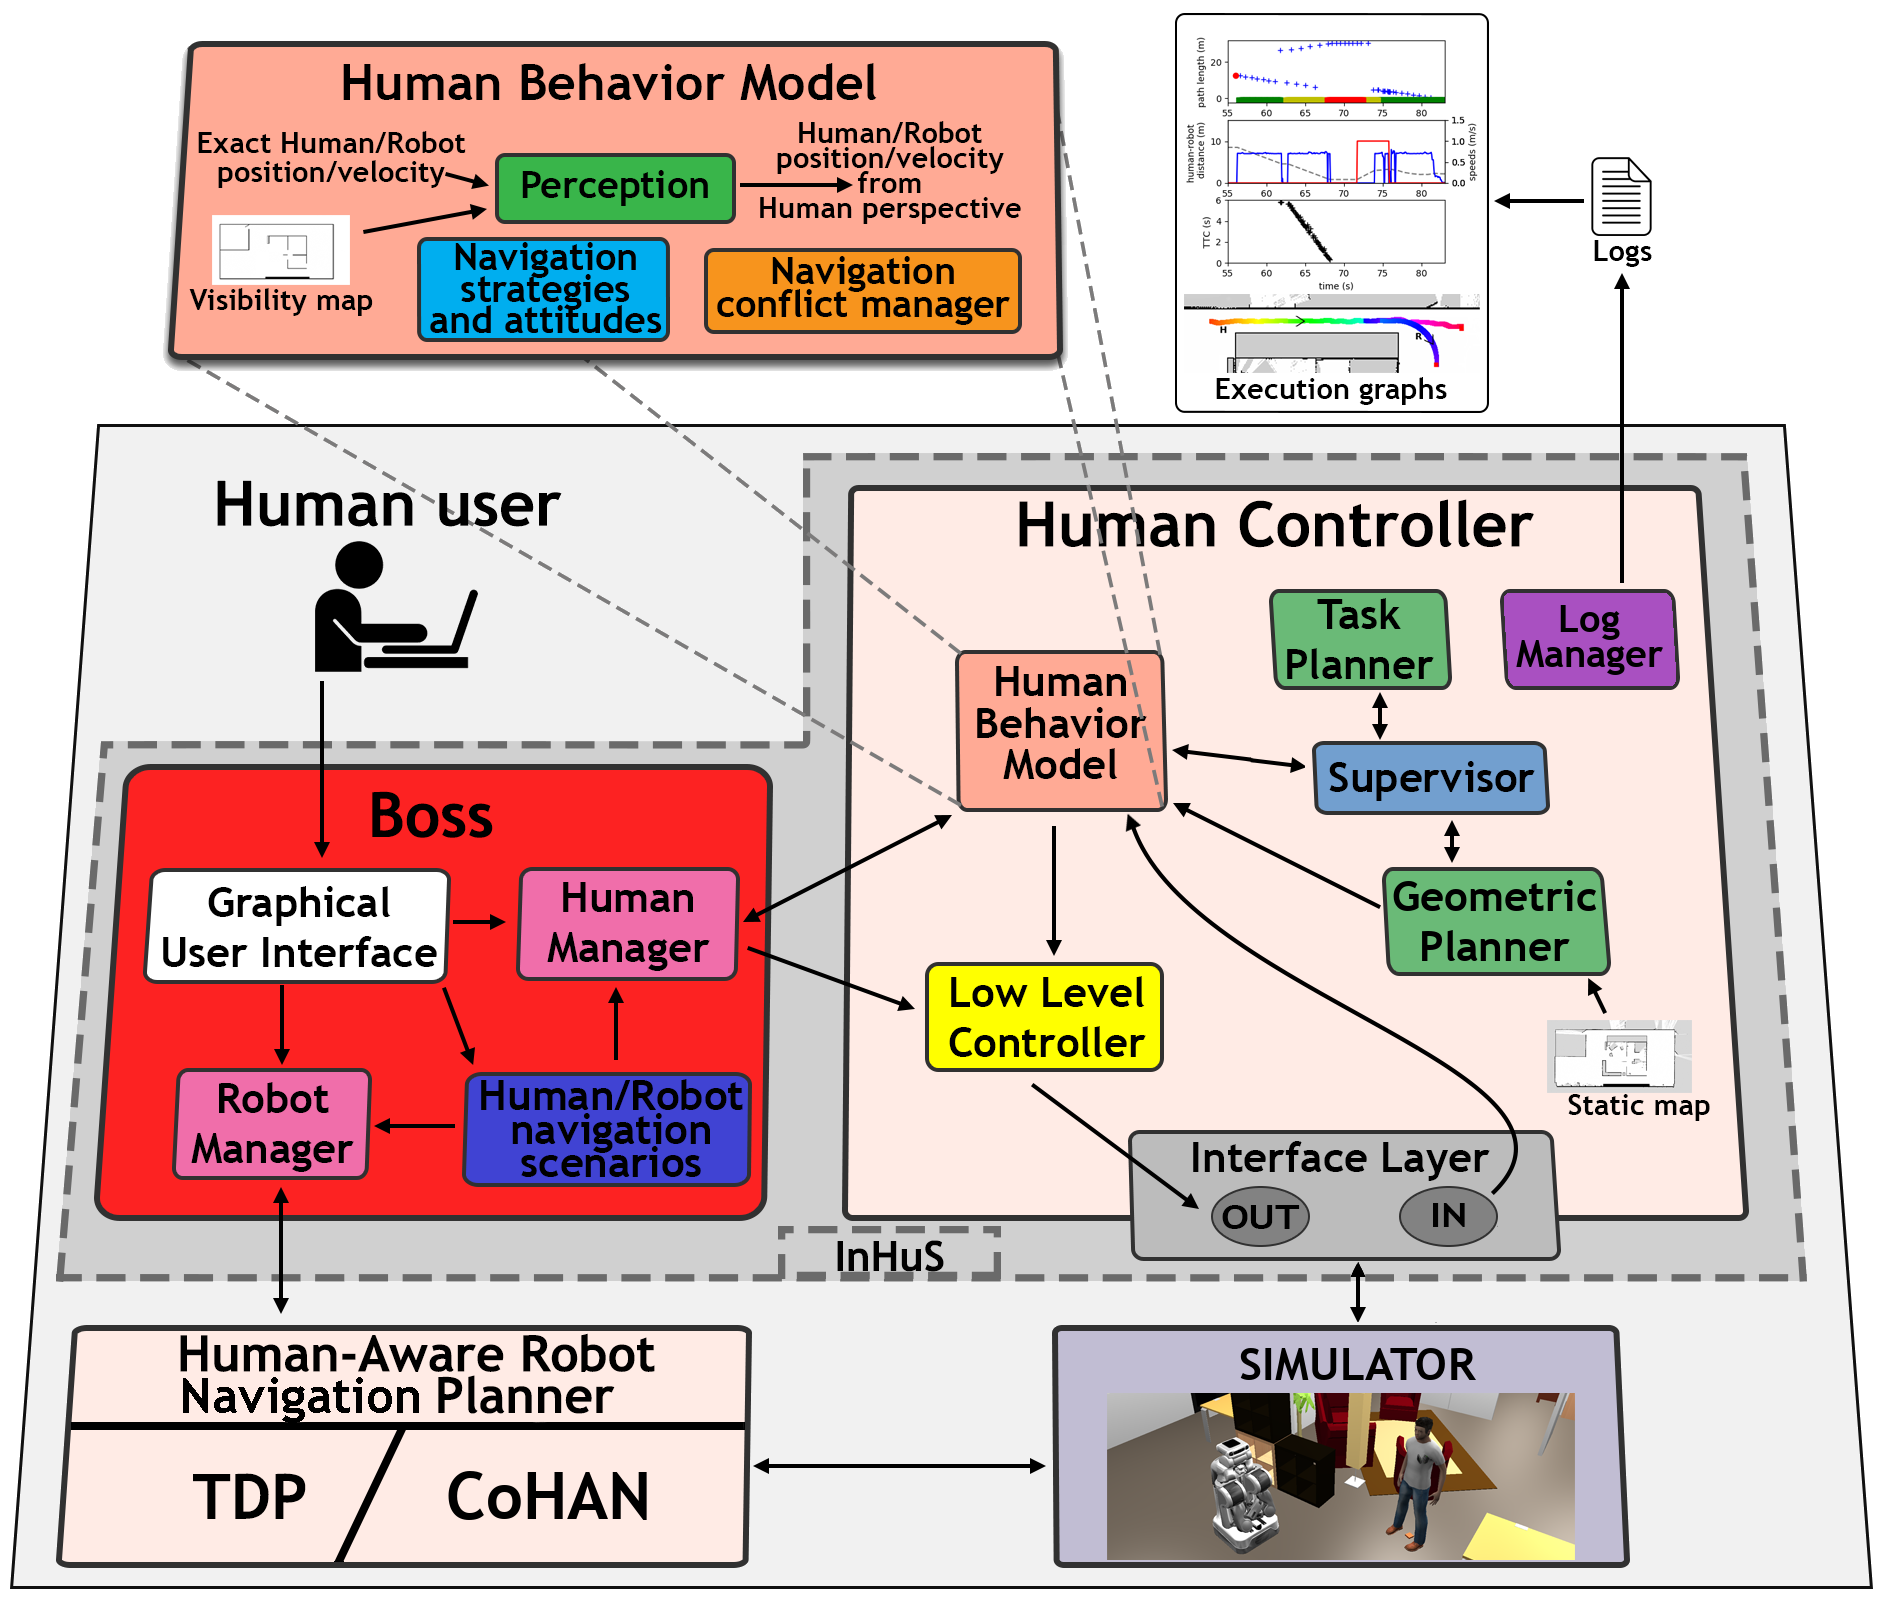
\includegraphics[width=0.9\columnwidth]{images/appendix/architecture.pdf}
    \caption{InHuS Architecture. The system consists of the Boss and the InHuS Human Controller macro components. The human operator interacts with the system through the Boss which in turn interacts with the Human Controller and the HAN Planner. Both the human and the robot controllers are connected to the same simulator where they control different components but share the same environment.}
    \label{fig:inhus}
\end{figure}
\subsection{Architecture}
The architecture of the proposed system is shown in Fig.~\ref{fig:inhus}. InHuS is composed of two major components namely, 1) \textit{Boss} and 2) \textit{Human Controller}. These components are explained in detail below:
\begin{itemize}[label={}]
    \item \textbf{Boss}: The \textit{Boss} component is responsible for taking input from the user and sending the appropriate instructions to the human and the robot planners. Hence it is provided with a graphical user interface through which a user can give individual goals to each agent, run or re-run predefined scenarios or initiate an endless loop of the human and robot navigating continuously from one goal to another. The endless loop can be used to identify the limits of the HAN system under test. After taking the input from the user, this component communicates the navigation goals to the \textit{Robot Manager} and \textit{Human Manager} at the appropriate times. Once the goals are communicated to these components, the \textit{Boss} does not interfere with the execution unless the human operator selects a new goal or scenario.
    \item \textbf{Human Controller}: This is the main component of InHuS that controls human motion and decides what to do in case of a conflict with the robot. It has an internal `\textit{Human Behaviour Model}' that makes these decisions and sets some attitudes to humans. The other major sub-component is the `\textit{Supervisor}', which supervises the execution of the goal and the progress, and activates the respective components as needed. While the `\textit{Geometric Planner}' provides the geometric path and trajectory to the goal, the `\textit{Low Level Controller}' sub-component sends the command velocity to the human avatar. The `\textit{Task Planner}' was used to define different kind of navigation tasks like \textit{go to goal}, \textit{wait} etc. Finally, the \textit{Log Manager} of this component logs the data and sends it to a GUI for visualisation of the calculated metrics.
\end{itemize}

\subsection{Supervisor and Geometric Planner}
The navigation goal of the human avatar is sent to the \textit{Supervisor}, which in turn asks the \textit{Task Planner} for a plan to achieve this goal. The \textit{Supervisor} then supervises and coordinates the execution of all the actions in the plan while managing the conflicts. The navigation plan generally consists of `moving' and `waiting' actions. This kind of architecture allows us to define complex navigation goals with multiple steps. The \textit{Supervisor} queries the \textit{Human Behaviour Model} from time to time to detect any potential conflicts. It has the power to suspend the execution of a plan in case of a conflict and resume it whenever necessary. This is especially useful to execute other actions in case of conflict to show the navigation intention and goal persistence of the human agent, unlike the reactive or simple planning approaches.

When the \textit{Supervisor} has to execute a `moving' action, it sends the navigation goal to the \textit{Geometric Planner}, which generates the path and then calculates the velocity commands to make the human move towards the goal. Depending on the type of trajectory planner selected, human motion can be different. In the current version, the standard \acrshort{ros} Navigation Stack or \acrshort{cohan} can be selected as the \textit{Geometric Planner}. The velocity command given by this component is not directly sent to the human. The \textit{Low Level Controller} receives this velocity and, if necessary, modifies or perturbs this velocity before sending it to the human avatar. This is used to emulate some reactions while navigation called `\textit{Attitudes}', which is presented in the next subsection.

\subsection{Human Behaviour Model}
The \textit{Human Behaviour Model} is the most important component of the proposed architecture. It controls the human avatar and is responsible for the behaviours exhibited by the human agent. As mentioned previously, this component manages the navigation conflicts, and in this version, only the blockage of the path by the robot is handled. Whenever the \textit{Geometric Planner} is called for the first time, the shortest path to the goal without any moving agents is calculated and sent to the `\textit{Navigation Conflict Manager}' of this component. If any blockage of this path by the robot is detected by this component, it changes the human state, and then the \textit{Supervisor} suspends the goal. The human avatar then performs an `approach' action where it moves towards the goal until it reaches a limiting distance from the robot. After this, it stops and waits for the robot to clear the way. Note that any collision avoidance or simple planning strategies will fail to show such behaviour as they will completely change the path of the human agent instead of showing persistence towards the goal.

This component can also set the goals for the human agent apart from the \textit{Boss}. The internal goal selection mechanism is responsible for different \textit{Attitudes} of the human avatar. Three kinds of attitudes are provided in InHuS:
\begin{enumerate}
    \item \textbf{Stop and Look}: It emulates a curious behaviour, where the human avatar navigating to the goal stops and looks at the robot shortly if the robot is in close vicinity of the human avatar. After this action, the navigation to the original goal is resumed.
    \item \textbf{Harass}: This attitude emulates a behaviour where the human avatar continuously disturbs the robot by blocking the robot's path. The idea here is to generate a child-like behaviour for the human avatar.
    \item \textbf{Random Goal}: In this attitude, a new random goal is set to the human avatar while it is already moving towards a goal, emulating something like a change of mind.
\end{enumerate}
To make the system more realistic, this module builds the perception of the human avatar using the map of the environment and the location of the other agents. The information about the other agents is taken directly from the simulator rather than using simulated cameras or lasers. Therefore, the human avatar does not consider the robot that it cannot see, even if it is below the threshold distance geometrically.

\subsection{Logs and Metrics}
The \textit{Log Manager} logs the data of the human-robot navigation interactions and sends it to GUI based data visualiser. This visualiser shows the different states of the human, the paths of the human and the robot, and some metrics to evaluate the robot's navigation. The logged data can also be used to calculate new metrics or methodologies for evaluation. A screenshot of this visualisation is shown in Fig. \ref{fig:gui_inhus}.
\begin{figure}[!ht]
    \centering
    \includegraphics[width=0.9\columnwidth]{images/appendix/gui_bis_bis.png}
    \caption{The data visualisation in GUI. On the right, the paths taken by the agents are shown, while on the left, the human states and the calculated metrics are shown.}
    \label{fig:gui_inhus}
\end{figure}
The paths shown on the right in Fig. \ref{fig:gui_inhus} are coloured over time. It means that the same colour on the paths represents the same time instant, and using this, one can interpret the behaviour of the agents better. On the left, the plot on the top shows the human avatar's distance to the goal and its estimated state over time. If no conflict occurs, the human stays in a single state, and the distance to the goal decreases linearly. The plots below the first one show some of the calculated metrics and the agents' velocities over time. One can calculate and add more metrics as needed using the logged data.

\subsection{Generating Different Behaviours}
\begin{figure}[!h]
    \centering
    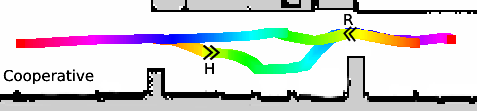
\includegraphics[width=0.9\columnwidth]{images/appendix/paths_coop_new.png}
    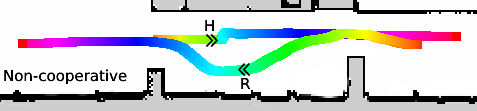
\includegraphics[width=0.9\columnwidth]{images/appendix/paths_stop_new.png}
    \caption{Traversed paths generated by InHuS during the Pillar corridor scenario. The top part is with cooperative settings and the bottom part with non-cooperative settings along with the \textit{Stop and Look} attitude.}
    \label{fig:paths_pillar_corridor_inhus}
\end{figure}
Depending on the \textit{Geometric Planner} and the \textit{Attitude}, different navigation behaviours can be emulated for the human avatar. For example, using the standard \acrshort{ros} Navigation stack and \textbf{Stop and Look} attitude, we can simulate a non-cooperative human who contributes nothing in a setting like a corridor. If \acrshort{cohan} is used, a cooperative yet curious human can be simulated. Moreover, \acrshort{cohan} can be tuned to set a degree of cooperative behaviour. The comparisons of different combinations and behaviours generated are presented in more detail in \cite{favier2021simulating}. Fig. \ref{fig:paths_pillar_corridor_inhus} shows the paths of the robot and human in two situations, one where the human is non-cooperative and curious and the other in which the human is completely cooperative.

% \section{ImHuS}

% \chapter{Effects of Social Constraints}
Each of the proposed social constraints in this thesis has some particular effect on the behaviour of the robot. Some of the predominant effects of these are briefly presented here. Each case presents a scenario without and with the social constraint activated. The figures of each scenario show the paths taken by the human and the robot (starting at blue and moving towards red) and their velocities (robot's velocity in red and human's velocity in blue) below. The velocity plot also includes the distance between the human and the robot during the execution of the scenario. 

\section{TTCplus Constraint}
\subsection{Approach}
\begin{figure}[!htb]
\centering
\begin{subfigure}{0.5\columnwidth}
  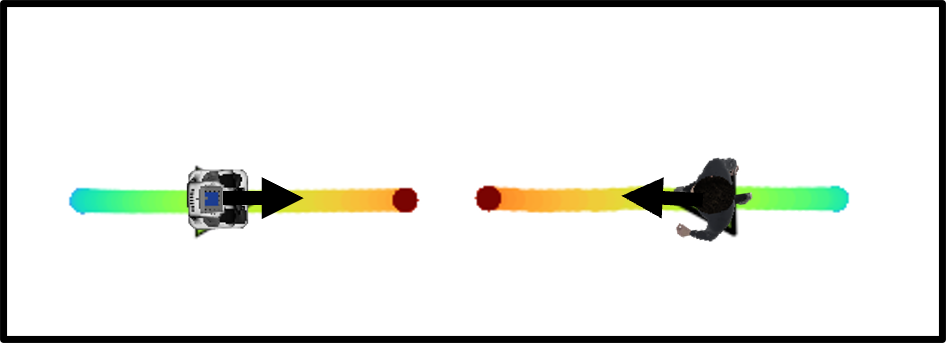
\includegraphics[width=\textwidth]{images/appendix/ttc/approach/approach_without.png}
\end{subfigure}
\vspace{0.5cm}
\begin{subfigure}{0.8\columnwidth}
  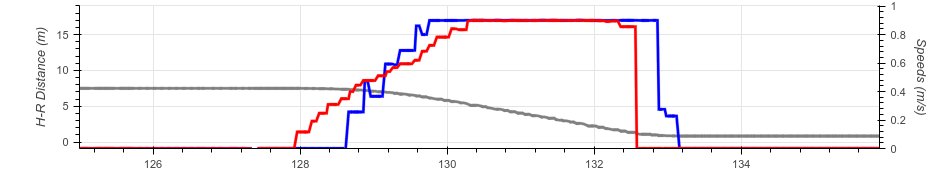
\includegraphics[width=\textwidth]{images/appendix/ttc/approach/without.png}
  \caption{without TTCplus}
\end{subfigure}

\begin{subfigure}{0.5\columnwidth}
  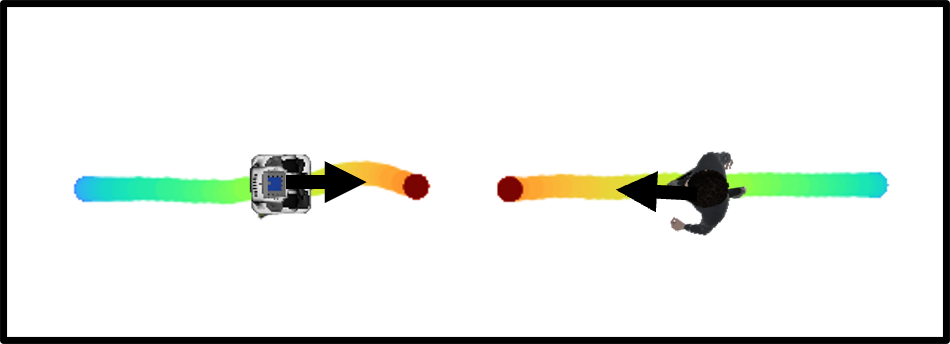
\includegraphics[width=\textwidth]{images/appendix/ttc/approach/approach_with.png}
\end{subfigure}
% \hspace{-0.75cm}
\begin{subfigure}{0.8\columnwidth}
  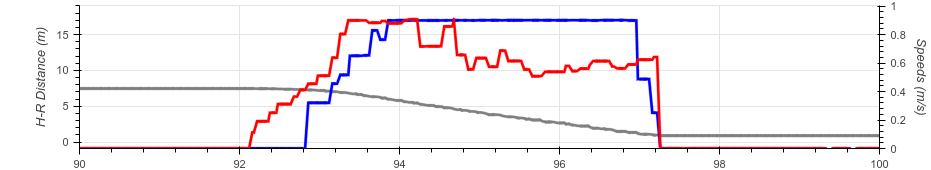
\includegraphics[width=\textwidth]{images/appendix/ttc/approach/with1.png}
  \caption{with TTCplus}
\end{subfigure}
\caption{The robot approaches a human head-on. The addition of the TTCplus constraint makes the robot deviate a little and slow down as it nears the human.}
\label{fig:approach_ttc}
\end{figure} 

In this scenario, the robot and human move towards each other and stop at a very close distance from each other. From Fig.~\ref{fig:approach_ttc} (a), it can be seen that the robot and human move at their full speeds towards each. However, with the addition of the TTCplus constraint, the robot has a decreasing velocity profile as the human-robot distance decreases, showing the robot's intention to stop (shown in Fig.~\ref{fig:approach_ttc} (b)).

\subsection{Open Space Crossing}
\begin{figure}[H]
\centering
\begin{subfigure}{0.5\columnwidth}
  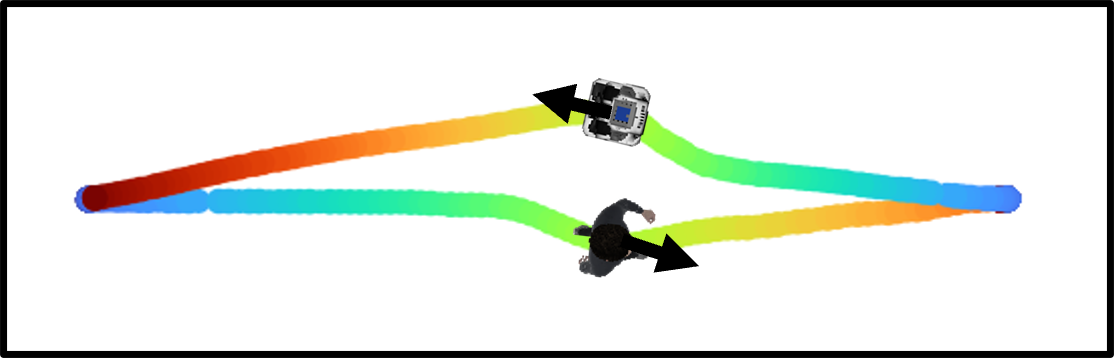
\includegraphics[width=\textwidth]{images/appendix/ttc/wide/without.png}
\end{subfigure}
\vspace{0.5cm}
\begin{subfigure}{0.8\columnwidth}
  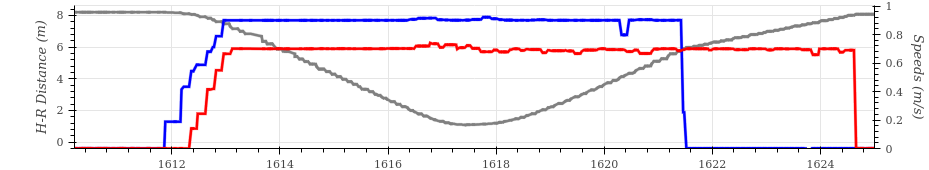
\includegraphics[width=\textwidth]{images/appendix/ttc/wide/wide_without1.png}
  \caption{without}
\end{subfigure}

\begin{subfigure}{0.5\columnwidth}
  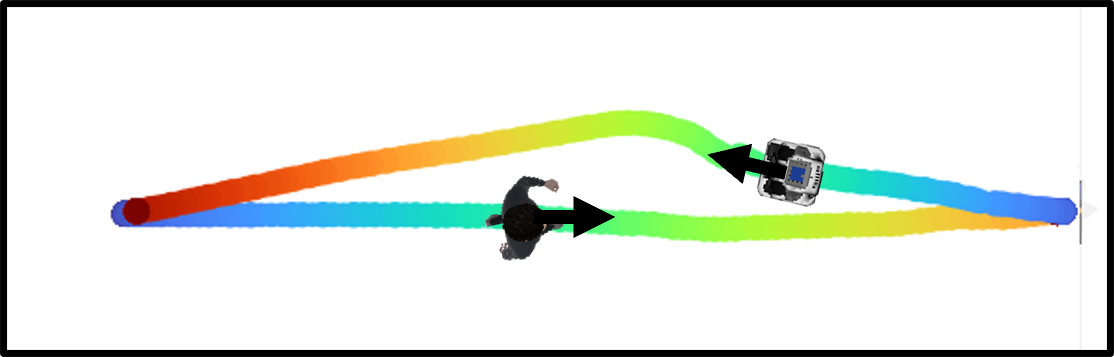
\includegraphics[width=\textwidth]{images/appendix/ttc/wide/with.png}
\end{subfigure}
% \hspace{-0.75cm}
\begin{subfigure}{0.8\columnwidth}
  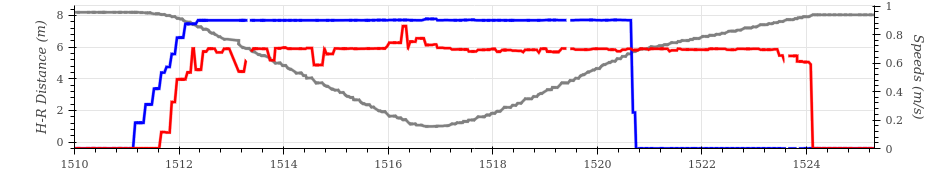
\includegraphics[width=\textwidth]{images/appendix/ttc/wide/wide_with2.png}
  \caption{with}
\end{subfigure}
\caption{The human and the robot cross each other in an open space. The addition of the TTCplus constraint makes the robot move aside quickly, showing its intention to give way and the choice of its side to move.}
\label{fig:open_space_ttc}
\end{figure} 

\hspace{\parindent} This scenario simulates a robot crossing a human in an open area where there is enough space to move away and not disturb the human. In Fig.~\ref{fig:open_space_ttc} (a), the robot and human move directly towards each other and only avoid each other at the last minute before the collision. This puts on an additional burden on the human to deviate from his path to avoid a collision with the robot. A more human-aware robot should avoid the occurrence of such path deviation, which is similar to what is seen in Fig.~\ref{fig:open_space_ttc} (b). Therefore, the TTCplus constraint not only shows its intention to move away early but also reduces the additional navigational burden that might be imposed on the human.  

\subsection{Corridor Crossing}
\begin{figure}[H]
\centering
\begin{subfigure}{0.5\columnwidth}
  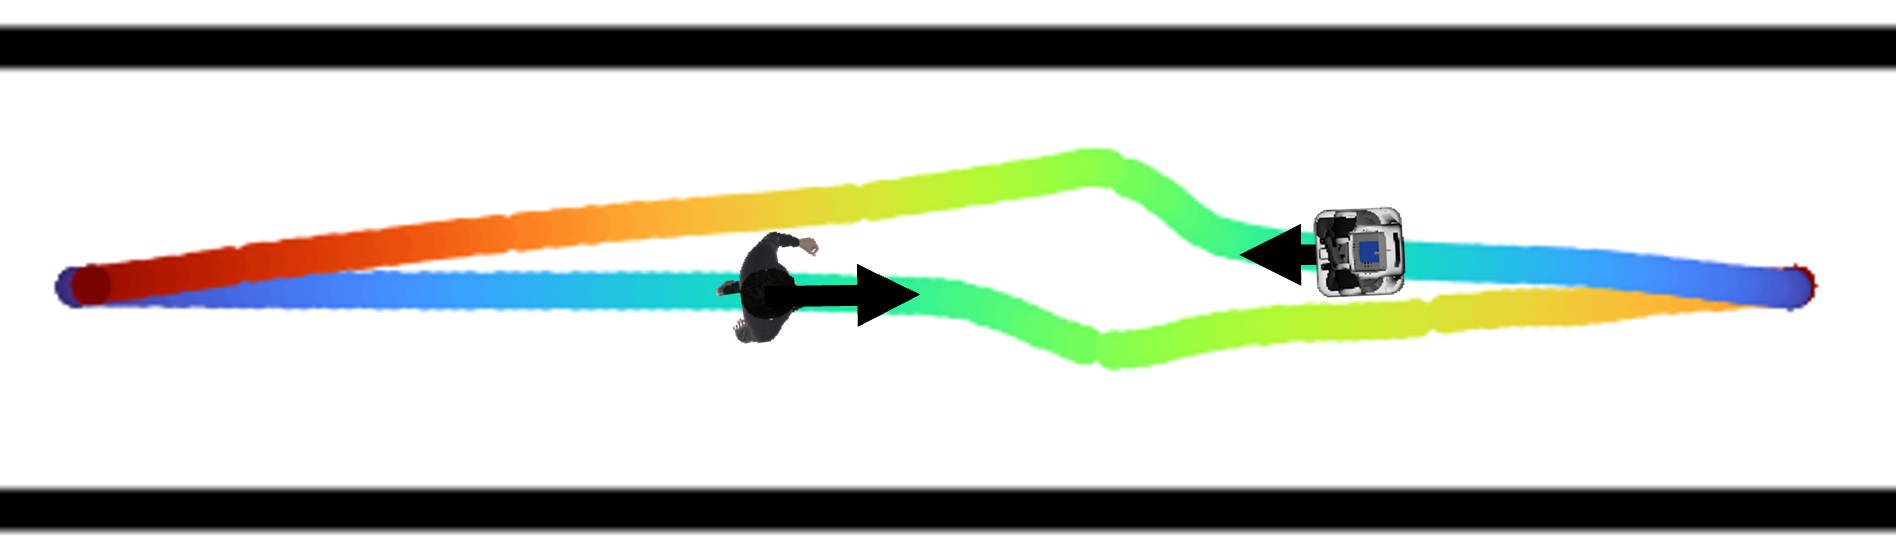
\includegraphics[width=\textwidth]{images/appendix/ttc/corridor/without.png}
\end{subfigure}
\vspace{0.5cm}
\begin{subfigure}{0.8\columnwidth}
  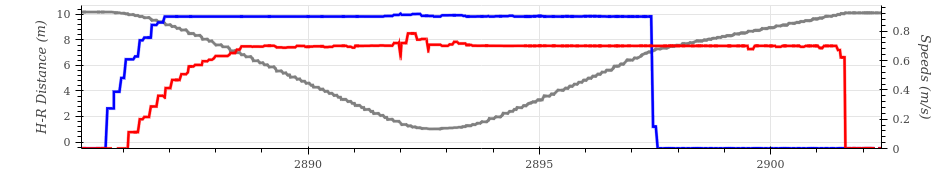
\includegraphics[width=\textwidth]{images/appendix/ttc/corridor/coor_without2.png}
  \caption{without}
\end{subfigure}

\begin{subfigure}{0.5\columnwidth}
  
\includegraphics[width=\textwidth]{images/appendix/ttc/corridor/with.png}
\end{subfigure}
% \hspace{-0.75cm}
\begin{subfigure}{0.8\columnwidth}
  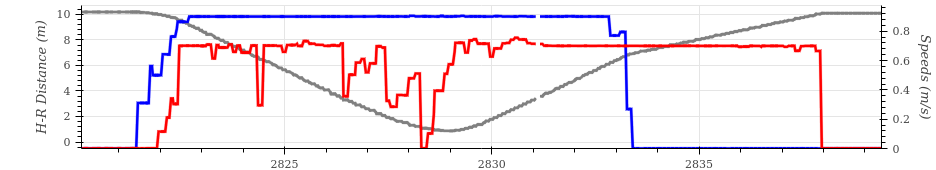
\includegraphics[width=\textwidth]{images/appendix/ttc/corridor/coor_with2.png}
  \caption{with}
\end{subfigure}
\caption{The human and the robot cross each other in a corridor. TTCplus constraint not only makes the robot take a side early but also slows down the robot as it crosses the human.}
\label{fig:corridor_ttc}
\end{figure} 

\hspace{\parindent} This scenario is similar to the previous one, but the space is narrower. As there is not enough space to move away, the robot with the TTCplus constraint moves to a side as well as slows down, as shown in Fig.~\ref{fig:corridor_ttc} (b). Without this constraint, it behaves exactly like in the previous case (Fig.~\ref{fig:corridor_ttc} (a)). 

\section{Relative Velocity Constraint}
\subsection{Corridor Crossing}
\hspace{\parindent} The corridor crossing scenario is the same as the one shown in the previous section. In the case of the Relative Velocity constraint, the robot should try to move away as quickly as possible and provide more space for the human even when the line of travel is not the same. This can be clearly seen from the path and the velocity profile of the robot in Fig.~\ref{fig:corridor_rel}. The robot starts to move to one side very quickly and slows down as it crosses the human. If there was enough space, the robot could have moved with a larger velocity while crossing. This constraint addresses parallel travel better when compared to TTCplus.

\begin{figure}[H]
\centering
% \begin{subfigure}{0.4\columnwidth}
%   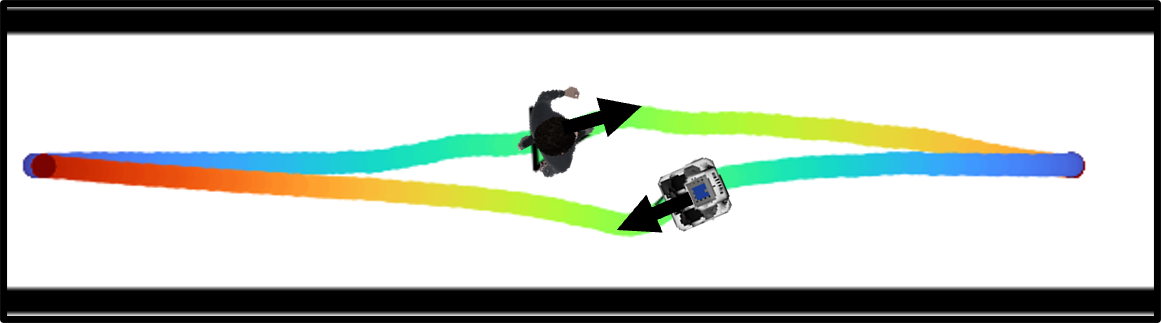
\includegraphics[width=\textwidth]{images/appendix/relvel/corridor/without.png}
% \end{subfigure}
% \vspace{0.5cm}
% \begin{subfigure}{0.8\columnwidth}
%   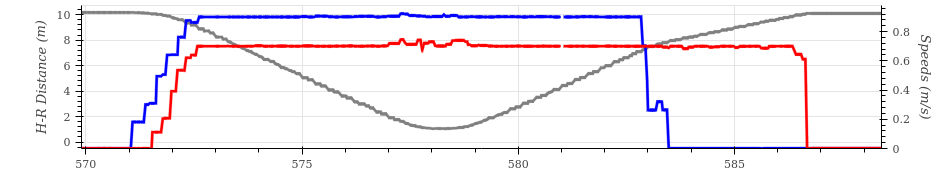
\includegraphics[width=\textwidth]{images/appendix/relvel/corridor/corr_without2.png}
%   \caption{without}
% \end{subfigure}

\begin{subfigure}{0.5\columnwidth}
  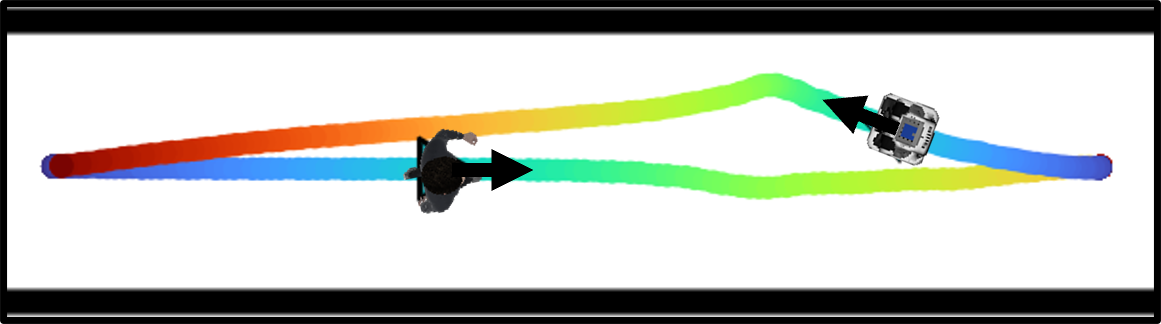
\includegraphics[width=\textwidth]{images/appendix/relvel/corridor/with.png}
\end{subfigure}
% \hspace{-0.75cm}
\begin{subfigure}{0.8\columnwidth}
  \includegraphics[width=\textwidth]{images/appendix/relvel/corridor/corr_with2.png}
  % \caption{with Relative Velocity Constraint}
\end{subfigure}
\caption{The human and the robot cross each other in a corridor. Relative Velocity constraint makes the robot clear the way quickly and move with a slower speed robot as it crosses the human at a small parallel distance.}
\label{fig:corridor_rel}
\end{figure} 

\subsection{Open Space Crossing}

\begin{figure}[H]
\centering
% \begin{subfigure}{0.4\columnwidth}
%   \includegraphics[width=\textwidth]{images/appendix/relvel/wide/without.png}
% \end{subfigure}
% \vspace{0.5cm}
% \begin{subfigure}{0.8\columnwidth}
%   \includegraphics[width=\textwidth]{images/appendix/relvel/wide/without2.png}
%   \caption{without}
% \end{subfigure}

\begin{subfigure}{0.5\columnwidth}
  \includegraphics[width=\textwidth]{images/appendix/relvel/wide/with.png}
\end{subfigure}
% \hspace{-0.75cm}
\begin{subfigure}{0.8\columnwidth}
  \includegraphics[width=\textwidth]{images/appendix/relvel/wide/with2.png}
  % \caption{with}
\end{subfigure}
\caption{The human and the robot cross each other in an open space. The addition of the Relative Velocity constraint makes the robot take a large deviation by exploiting the available space while showing its intention to give way. It also facilitates the robot to move at a larger velocity towards the goal.}
\label{fig:wide_rel}
\end{figure}

\hspace{\parindent} In this setting, the robot has enough space to move away and then travel with a larger velocity. Without the addition of the Relative Velocity constraint, the robot and human avoid each other moments before the collision, similar to Fig.~\ref{fig:open_space_ttc} (a). This constraint makes the robot move away very quickly and exploit the available space to move at full speed towards its goal. It can be observed from the path and the speed profile of the robot in Fig.~\ref{fig:wide_rel}. This clearly shows how the Relative Velocity constraint addresses the parallel travel better compared to the TTCplus constraint (see Fig.~\ref{fig:open_space_ttc} (b)).

\section{Visibility Constraint}
\hspace{\parindent} To show the advantage of adding the visibility constraint, an overtaking scenario is simulated. In this setting, the robot encounters a human moving very slowly and partially blocking its way. The robot has to over the human in order to move to its goal faster. In the first case, shown in Fig.~\ref{fig:visib_const} (a), without the addition of Visibility constraint, the robot overtakes the human very closely and also disturbs his navigation. With the addition of this constraint, however, the robot takes a large deviation and tries to enter the human's field of view as far as possible without disturbing him. This can be observed from the plots in Fig.~\ref{fig:visib_const} (b).
\begin{figure}[H]
\centering
\begin{subfigure}{0.5\columnwidth}
  \includegraphics[width=\textwidth]{images/appendix/vis/without.png}
\end{subfigure}
\vspace{0.5cm}
\begin{subfigure}{0.8\columnwidth}
  \includegraphics[width=\textwidth]{images/appendix/vis/without1.png}
  \caption{without}
\end{subfigure}

\begin{subfigure}{0.5\columnwidth}
  \includegraphics[width=\textwidth]{images/appendix/vis/with.png}
\end{subfigure}
% \hspace{-0.75cm}
\begin{subfigure}{0.8\columnwidth}
  \includegraphics[width=\textwidth]{images/appendix/vis/with2.png}
  \caption{with}
\end{subfigure}
\caption{The robot overtakes a human who is moving very slowly. The addition of the Visibility constraint makes the robot enter the human's field of view slowly without surprising or disturbing the human.}
\label{fig:visib_const}
\end{figure}

\section{Updated Invisible Humans Constraint}
\hspace{\parindent} As shown in chapter~\ref{chap:5}, the current version of the `Invisible Humans' constraint already addresses a lot of scenarios to proactively accommodate sudden human appearances. However, the defined formulation had some issues which needed to be addressed using passage detection and mode shifting. After testing the robot navigation in more complicated scenarios, we observed that the current formulation could lead to some deadlocks even after the passage detection. One such deadlock situation is shown in Fig.~\ref{fig:inv_fail}. Here, the robot faces opposing forces from the obstacles and the invisible humans and freezes before it can even detect an opening.
\begin{figure}[h]
    \centering
    \includegraphics[width=0.8\columnwidth]{images/appendix/inv/updated_inv.png}
    \caption{A situation where the current formulation of the Invisible Humans constraint could fail. The opposing forces from the obstacles and the invisible humans make the robot freeze without moving.}
    \label{fig:inv_fail}
\end{figure}
Therefore, we update our formulation by taking inspiration from the Relative Velocity constraint. Instead of using the velocity of the visible humans, we use the defined invisible humans' velocity in the formulation and update the formulation as follows:
\begin{equation}
\begin{split}
cost_{inv\_human} &= max\left(\frac{V-a\Delta t_n+\lVert\overrightarrow{V_r}\rVert+1}{d}, 0\right)\quad \text{if}\quad \Delta t_n> 0.5s\\
                &= \frac{V}{d}\quad otherwise
\end{split}
\label{updated_inv_eq}
\end{equation}

In the latest version of CoHAN, the above formulation is used instead of the previous one. The rigorous testing of the updated formulation is still pending, but we already see some improvements over the previous one. An example of the constrained door crossing is presented below.

\subsection{Testing the Updated Constraint}
\hspace{\parindent} The above formulation acts on the robot's velocity during the possible freezing scenarios and makes the robot move with lower velocities, and reduces the cost. Since it is an updated formulation of the Invisible Humans constraint, it should still hold the properties of the previous formulation. To show this, we have simulated the door crossing scenario again with a wall on the side that limits the space. 

In Fig.~\ref{fig:door_inv_new} (a), the robot moves without considering and accounting for the invisible humans in the environment. Therefore, it moves at almost full speed and takes the shortest path to reach the goal. With the formulation in chapter~\ref{chap:5}, the robot froze between the wall and the entry to the door and did not move. However, with the updated formulation, the robot moves away from the door as much as possible without colliding with the wall and also aligns itself to properly pass through the door. Further, while crossing the door, the robot moves very cautiously with a slower velocity, as seen in Fig.~\ref{fig:door_inv_new} (b) between $140-145 s$.
\begin{figure}[!ht]
\centering
\begin{subfigure}{0.3\columnwidth}
  \includegraphics[width=\textwidth]{images/appendix/inv/without.png}
\end{subfigure}
\vspace{0.5cm}
\begin{subfigure}{0.8\columnwidth}
  \includegraphics[width=\textwidth]{images/appendix/inv/without2.png}
  \caption{Without Invisible Humans constraint}
\end{subfigure}

\begin{subfigure}{0.3\columnwidth}
  \includegraphics[width=\textwidth]{images/appendix/inv/with.png}
\end{subfigure}
% \hspace{-0.75cm}
\begin{subfigure}{0.8\columnwidth}
  \includegraphics[width=\textwidth]{images/appendix/inv/with2.png}
  \caption{with the updated Invisible Humans constraint}
\end{subfigure}
\caption{Constrained door crossing scenario. The robot has to enter a door in a narrow space and try to accommodate humans as much as possible. The updated Invisible Humans constraint makes the robot move close to the wall before aligning itself towards the door and carefully entering it.}
\label{fig:door_inv_new}
\end{figure}

%%%%%%%%%%%Need to update this%%%%%%%
% \include{Annexe_fr_long}

\bibliographystyle{StyleThese}
% \bibliographystyle{plain}
% \bibliographystyle{unsrt}
%%%%%%%%%%%%Need to update this%%%%%%%%%%%%
\bibliography{These-refs}

% \cleardoublepage
% \begin{vcenterpage}
% \noindent\rule[2pt]{\textwidth}{0.5pt}

% % 1700 à 4000 caractères

% \textbf{Abstract:}
% %%%%%%%%%%%%%%%%%%%%%% ATTENTION ! SI MODIFICATION => MODIF SUR ADUM AUSSI !!!

% %%%%%%%%%%%%%Need to update this%%%%%%%%%%%%%%%%%%5
% \textcolor{red}{As robots begin to enter our daily lives, we need advanced knowledge representations and associated reasoning capabilities to enable them to understand and model their environments. Considering the presence of humans in such environments, and therefore the need to interact with them, this need comes with additional requirements. Indeed, knowledge is no longer used by the robot for the sole purpose of being able to act physically on the environment but also to communicate and share information with humans. Therefore knowledge should no longer be understandable only by the robot itself, but should also be able to be narrative-enabled. 
% In the first part of this thesis, we present our first contribution with Ontologenius. This software allows to maintain knowledge bases in the form of ontology, to reason on them and to manage them dynamically. We start by explaining how this software is suitable for \acrfull{hri} applications. To that end, for example to implement theory of mind abilities, it is possible to represent the robot’s knowledge base as well as an estimate of the knowledge bases of human partners. We continue with a presentation of its interfaces. This part ends with a performance analysis, demonstrating its online usability. 
% In a second part, we present our contribution to two knowledge exploration problems around the general topic of spatial referring and the use of semantic knowledge. We start with the route description task which aims to propose a set of possible routes leading to a target destination, in the framework of a guiding task. To achieve this task, we propose an ontology allowing us to describe the topology of indoor environments and two algorithms to search for routes. The second knowledge exploration problem we tackle is the \acrfull{reg} problem. It aims at selecting the optimal set of piece of information to communicate in order to allow a hearer to identify the referred entity in a given context. This contribution is then refined to use past activities coming from joint action between a robot and a human, in order to generate new kinds of Referring Expressions. It is also linked with a symbolic task planner to estimate the feasibility and cost of future communications. 
% We conclude this thesis by the presentation of two cognitive architectures. The first one uses the route description contribution and the second one takes advantage of our Referring Expression Generation contribution. Both of them use Ontologenius to manage the semantic Knowledge Base. Through these two architectures, we present how our contributions enable Knowledge Base to gradually take a central role, providing knowledge to all the components of the architectures.}

% \textbf{Keywords:} human-robot interaction, Human-Aware Navigation, Social Navigation
% \\
% \noindent\rule[2pt]{\textwidth}{0.5pt}
% \end{vcenterpage}

\end{document}
